\documentclass[11pt,letterpaper]{article}
\usepackage[margin=1in]{geometry}
\usepackage[T1]{fontenc}
\usepackage{lmodern,amsmath,amssymb,amsthm,mathtools,booktabs,array,tikz}
\usepackage{enumitem}
\usetikzlibrary{arrows.meta,positioning,fit,backgrounds}
\usepackage[colorlinks=true,linkcolor=blue,citecolor=blue,urlcolor=blue]{hyperref}
\usepackage[nameinlink,noabbrev]{cleveref}
\renewenvironment{abstract}{\par\medskip\normalsize\leftskip=0pt\rightskip=0pt\parfillskip=0pt plus 1fil\parindent=1em\noindent\textbf{Abstract}\par\medskip\ignorespaces}{\par}
\setlength{\parskip}{3pt}
\setlength{\parindent}{1em}
\newcommand{\Q}{\mathbb{Q}}
\newcommand{\Qb}{\overline{\mathbb{Q}}}
\newcommand{\N}{\mathbb{N}}
\newcommand{\Z}{\mathbb{Z}}
\newcommand{\cG}{\mathcal{G}}
\newcommand{\cK}{\mathcal{K}}
\newcommand{\cH}{\mathcal{H}}
\newcommand{\cW}{\mathcal{W}}
\newcommand{\cA}{\mathcal{A}}
\newcommand{\cY}{\mathcal{Y}}
\newcommand{\fu}{\mathfrak{u}}
\newcommand{\fg}{\mathfrak{g}}
\newcommand{\im}{\operatorname{im}}
\newcommand{\id}{\operatorname{id}}
\newcommand{\spn}{\operatorname{span}}
\newcommand{\GL}{\mathrm{GL}}
\newcommand{\eps}{\varepsilon}
\newcommand{\tr}{\operatorname{tr}}
\newcommand{\vecop}{\operatorname{vec}}
\newcommand{\res}{\operatorname{res}}
\newcommand{\bin}{\mathrm{bin}}
\newtheorem{theorem}{Theorem}
\newtheorem{lemma}[theorem]{Lemma}
\newtheorem{proposition}[theorem]{Proposition}
\newtheorem{corollary}[theorem]{Corollary}
\theoremstyle{definition}
\newtheorem{definition}[theorem]{Definition}
\newtheorem{example}[theorem]{Example}
\newtheorem{remark}[theorem]{Remark}
\hypersetup{pdftitle={Copyless Cost Register Automata and Algebraic Groups: Exact Characterization for Invertible Series, Efficient Decision, and Non-Closure under Reversal},pdfauthor={Zijian Zeng, Jiayin Cao, Weinan Dai, Rui Wang, Fei Ding},pdfkeywords={copyless cost register automata, weighted automata, rational series, linear algebraic groups, Zariski closure}}
\begin{document}
\begin{titlepage}
\centering
{\Large\bfseries Copyless Cost Register Automata and Algebraic Groups:\par}
\medskip
{\large\bfseries Exact Characterization for Invertible Series, Efficient Decision, and Non-Closure under Reversal\par}
\vspace{1.8em}
{\renewcommand{\arraystretch}{1.1}%
\begin{tabular}{@{}c@{\hspace{2em}}c@{\hspace{2em}}c@{}}
{\large Zijian Zeng} & {\large Jiayin Cao} & {\large Weinan Dai}\\
UCSI University & Ningbo University & Zhejiang University\\
{\small\href{mailto:1002266693@ucsiuniversity.edu.my}{1002266693@ucsiuniversity.edu.my}} &
{\small\href{mailto:2795820153@qq.com}{2795820153@qq.com}} &
{\small\href{mailto:21725058@zju.edu.cn}{21725058@zju.edu.cn}}
\end{tabular}\par\bigskip
\begin{tabular}{@{}c@{\hspace{3em}}c@{}}
{\large Rui Wang} & {\large Fei Ding}\\
Nanchang Institute of Technology & Alibaba Group\\
{\small\href{mailto:2002007@nut.edu.cn}{2002007@nut.edu.cn}} &
{\small\href{mailto:dingfei@email.ncu.edu.cn}{dingfei@email.ncu.edu.cn}}
\end{tabular}\par}
\vspace{1.5em}
\begin{abstract}
Copyless cost register automata (CCRA) process a word with finite control and polynomial register updates in which each stored value is used at most once. Which rational weighted-automaton functions admit such a resource restriction? We give an exact answer when the letter matrices of the minimal linear representation are invertible, and we prove two conjectures of Mazowiecki, Puch and Smertnig: their uniform pumping condition is not sufficient for CCRA-computability, and CCRA over $\Q$ are not closed under reversal.

Let $\cG$ be the Zariski closure of the group generated by these matrices. Such a series is CCRA-computable if and only if $\cG^\circ$ is triangularizable over $\Q$ and any two unipotent elements of $\cG$ commute. Every such series admits permutation control and isolated affine updates $x:=\alpha x+\beta$, with registers combined only at output. The proof compresses arbitrary copyless updates to affine coordinate permutations and uses return blocks to transfer their group structure through finite control.

Consequences include reversal closure and an exact relation to polynomial ambiguity: an invertible series is polynomially ambiguous if and only if $\cG^\circ$ is triangularizable over $\Q$ (an intrinsic form of a characterization of Puch and Smertnig), so CCRA-computability adds exactly the commutation of unipotent elements, and polynomial ambiguity of invertible series is decidable in deterministic polynomial time. Membership is decidable in deterministic polynomial time, by a procedure that avoids Zariski-closure computation. In the unipotent class, membership reduces to commutation of the minimal letter matrices and is decidable in polynomial time. We also prove that the position-sum candidate of Mazowiecki, Puch and Smertnig, which satisfies their uniform pumping condition, has no CCRA realization. Beyond the invertible class, the witness for non-closure under reversal is $\sum_{i}\prod_{j<i}|u_j|$ over blocks $u_0\#u_1\#\cdots$: it is not CCRA-computable, while its reversal is. The obstruction is arithmetic: a compressed register must carry the inverse of a weight of the unipotent part. We also characterize CCRA-computability exactly when all singular minimal letter matrices have rank at most one, and for one invertible letter with a rank-two reset such that every word containing the reset has rank two. A characterization for arbitrary singular series remains open.
\end{abstract}
\end{titlepage}
\thispagestyle{empty}
{\small\hypersetup{linkcolor=black}\tableofcontents}
\thispagestyle{empty}
\clearpage
\setcounter{page}{1}

\section{Introduction}\label{sec:intro}
\paragraph{Copyless registers.}
A finite automaton reads its input once, from left to right, with constant memory. Equipping it with finitely many registers that hold values from a semiring, and updating them at each step by expressions in the old values, yields the cost register automata (CRA) of Alur, D'Antoni, Deshmukh, Raghothaman and Yuan~\cite{ADDRY13}. Over a field, CRA with linear updates are exactly weighted automata, whereas unrestricted polynomial updates such as $x:=x^2$ leave the realm of rational series. The \emph{copyless} restriction requires that every old register is used at most once in each update and at most once in the output. It originates in streaming string transducers, where copyless register updates capture exactly the MSO-definable, or regular, string-to-string functions~\cite{AC10,AC11}. Copylessness is a resource-linearity discipline: a stored value may be moved, combined with others, or discarded, but never duplicated. It is the register-machine analogue of an affine type discipline, in which every variable is used at most once.

Over a field, copyless polynomial CRA (CCRA) compute only rational series~\cite{MR16,MR19,MPS26}: substituting copyless updates into squarefree monomials produces squarefree polynomials, so the induced action on multiaffine polynomials is linear (Section~\ref{sec:prelim}). As noted in~\cite{MPS26}, CCRA and polynomially ambiguous weighted automata are the richest studied classes known to lie strictly between deterministic and general weighted automata. Over $\Q$ and a one-letter alphabet both classes coincide with the linear recurrence sequences for which every root $\lambda$ of the minimal recurrence satisfies $\lambda^k\in\Q$ for some $k\ge1$~\cite{BFLM22}. Over larger alphabets they are incomparable~\cite{MPS26}.

Which rational series are computed by CCRA? Mazowiecki, Puch and Smertnig~\cite{MPS26} proved a uniform pumping condition necessary for CCRA, used it to separate CCRA from polynomially ambiguous automata, and conjectured that this condition is not sufficient.\footnote{We cite numbered results from the conference version~\cite{MPS26}. The full version~\cite{MPSfull} numbers Definition~11, Theorem~15, Example~17, Theorem~18, Section~3.2 and Examples~26--27 identically; Lemma~50, Appendix~B.4, Conjecture~51 and Example~52 are cited from there.} They proposed a position-sum candidate whose nonrecognizability they could not prove, and suggested that in some sense a characterization should not exist, partly because CCRA are expected not to be closed under reversal (as is the case over the tropical semiring~\cite{MR16}); we confirm this over $\Q$ in Section~\ref{sec:singular}. The unipotent case of our results (Theorem~\ref{thm:sectors}(1)) already settles the candidate.

\paragraph{Main result.}
Every rational series $f:\Sigma^*\to\Q$ has a minimal linear representation $f(w)=\lambda M_w\gamma$, unique up to simultaneous conjugation, where $M_{a_1\cdots a_n}=M_{a_1}\cdots M_{a_n}$. We call $f$ \emph{invertible} if its minimal letter matrices are invertible. Let $\Gamma_f\le\GL_d(\Q)$ be the group they generate and $\cG_f$ its Zariski closure, a linear algebraic group with identity component $\cG_f^\circ$. A group of matrices is \emph{triangularizable over $\Q$} if some basis of $\Q^d$ makes all of its elements upper triangular.

\begin{theorem}[Main theorem]\label{thm:main}
For an invertible rational series $f:\Sigma^*\to\Q$ the following are equivalent.
\begin{enumerate}
\item[(C1)] $f$ is computed by a deterministic finite-state polynomial CCRA over $\Q$.
\item[(C2)] $f$ is computed by a CCRA whose control is a permutation automaton, in which every register is updated in isolation by a map $x\mapsto\alpha x+\beta$ with $\alpha\in\Q^\times$, $\beta\in\Q$, and whose outputs are linear combinations of products of distinct registers.
\item[(C3)] $\cG_f^\circ$ is triangularizable over $\Q$, and any two unipotent elements of $\cG_f$ commute.
\item[(C4)] $\Gamma_f$ has a subgroup of finite index that is triangularizable over $\Q$ and in which any two elements have commuting unipotent Jordan parts.
\end{enumerate}
Moreover, every function computed by a machine as in~(C2) is invertible.
\end{theorem}

Condition~(C3) is intrinsic, because minimal representations are unique up to conjugation. In~(C1) the competing machines are unrestricted CCRA: arbitrary finite control, any number of registers, arbitrary rational constants, and singular, resetting, merging or multiplicative updates. Condition~(C2) supplies a constructive realization of the intrinsic criterion. This normal form includes exponential growth, finite-state phenomena such as alternating sums, and the function $\sum_i2^ib_i$ on bit strings, for which Mazowiecki, Puch and Smertnig gave a dedicated construction~\cite[Example~27]{MPS26}; its group is the Baumslag--Solitar group $BS(1,2)$, which is not virtually nilpotent. The Zariski closure in~(C3) cannot be replaced by $\Gamma_f$ itself: for $f(w)=2^{|w|_a}3^{|w|_b}[w:ab]$, where $[w:ab]$ counts scattered occurrences of $ab$, all unipotent elements of $\Gamma_f$ are central, yet $f$ is not CCRA-computable (Example~\ref{ex:heis}).

\paragraph{Scope and significance.}
Copylessness formalizes a constraint on streaming computation: a register value can contribute to at most one updated register. The problem is to recognize this resource restriction from the function computed, rather than from a particular implementation. A weighted representation can conceal redundant memory, so the criterion must use its minimal representation. Theorem~\ref{thm:main} gives such an intrinsic test together with an explicit machine construction. It applies to the invertible class, for which Puch and Smertnig~\cite{PS24} characterize finite and polynomial ambiguity by arithmetic conditions; our criterion is group-theoretic. The method, which reads a syntactic resource restriction off the Zariski closure of the group generated by the minimal representation, does not depend on the details of registers. We expect it to be useful for other syntactic restrictions on data flow in streaming and resource-linear models.

Invertibility means that no input letter erases information in the minimal linear state. It permits accumulation, exponential scaling and finite permutations, including the running example below, but it excludes genuine resets in the minimal representation. This restriction is substantial: the full characterization remains open in the singular class, where CCRA are not closed under reversal (Corollary~\ref{cor:reversal}). There, Corollary~\ref{cor:local} gives a local necessary condition. If $f$ is CCRA-computable and a word $e$ satisfies $\operatorname{rank}M_e^2=\operatorname{rank}M_e$ and the blocks $eze$ act invertibly on the row space of $M_e$, then the Zariski closure of the group they generate satisfies~(C3). For instance, any finite set of words whose minimal matrices are invertible generates a group whose closure satisfies~(C3), even when other letters are singular.

The invertible CCRA series are exactly the series computed by reversible CCRA, while the necessity direction (C1)$\Rightarrow$(C3) holds against arbitrary machines.

\begin{corollary}[Reversible machines]\label{cor:reversible}
Call a CCRA \emph{reversible} if its control is a permutation automaton and every update $P_{s,a}$ is a bijection of $\Q^r$. A rational series is invertible and CCRA-computable if and only if it is computed by a reversible CCRA.
\end{corollary}
\begin{proof}
We use the notation of Section~\ref{sec:prelim}. A copyless polynomial bijection $P$ of $\Q^r$ is an affine coordinate permutation: no coordinate of $P$ is constant, since otherwise its image lies in a hyperplane; distinct coordinates have disjoint variable supports (Section~\ref{sec:prelim}), so each of the $r$ coordinates depends on exactly one of the $r$ variables, and a multiaffine polynomial in one variable has the form $\alpha x+\beta$, with $\alpha\ne0$ since the coordinate is nonconstant. Hence $P^{-1}$ is again copyless and $B_P$ is invertible on $V_r$ with inverse $B_{P^{-1}}$. As the control permutes $S$, the letter operators $(B_ah)_s=h_{\delta(s,a)}\circ P_{s,a}$ of the linearization in Section~\ref{sec:prelim} are invertible. The minimal representation is an invariant subquotient of the linearization, so its letter matrices are invertible. Conversely, the machines in Theorem~\ref{thm:main}(C2) are reversible. This also proves the last sentence of Theorem~\ref{thm:main}.
\end{proof}

Outside the invertible class the reading direction matters: CCRA over $\Q$ are not closed under reversal (Corollary~\ref{cor:reversal}), whereas polynomially ambiguous weighted automata are, as one sees by reversing the automaton; this is an obstruction of a different kind from pumping. Deciding whether a rational series lies in a subclass, such as the series of deterministic, unambiguous or polynomially ambiguous automata, is an active line of work~\cite{BS21,BS23,JMP24,PS24}, and our results add CCRA to this list for invertible series. For the general question, Mazowiecki, Puch and Smertnig suggested that a characterization might not exist~\cite{MPS26}; our results show that one exists for invertible series, while non-closure under reversal shows that no characterization of all CCRA series can be invariant under transposition of the minimal representation (Remark~\ref{rem:localcond}).

\paragraph{Running example and a forbidden pattern.}
Consider $\bin(b_1\cdots b_n)=\sum_{i=1}^n2^i b_i$. The one-state CCRA of Figure~\ref{fig:machine}(a) starts with $h=0$, $p=1$ and, on reading $b$, performs the simultaneous updates $h:=h/2+b$ and $p:=2p$. After $n$ letters,
\[
p_n=2^n,\qquad h_n=\sum_{i=1}^n2^{i-n}b_i,\qquad h_np_n=\bin(b_1\cdots b_n).
\]
Each old register appears once across the two updates and once in the output, so multiplying the registers at output copies neither of them. The generated group is noncommutative, because scaling by $2$ does not commute with translation; Theorem~\ref{thm:main} permits this. Figure~\ref{fig:machine}(b) shows what it forbids. For the position sum $\sum_i i\,b_i$ of~\cite[Example~26]{MPS26}, the natural machine keeps the current position $\ell$ and, on reading $1$, performs $s:=s+\ell$ and $\ell:=\ell+1$, which reads $\ell$ twice. Here $\ell$ accumulates additively and $s$ accumulates $\ell$. In the minimal representation the two letters act by unipotent matrices that do not commute, and Theorem~\ref{thm:sectors}(1) shows that no CCRA computes this function, whatever finite control, registers and update polynomials it uses.

\begin{figure}[t]
\centering
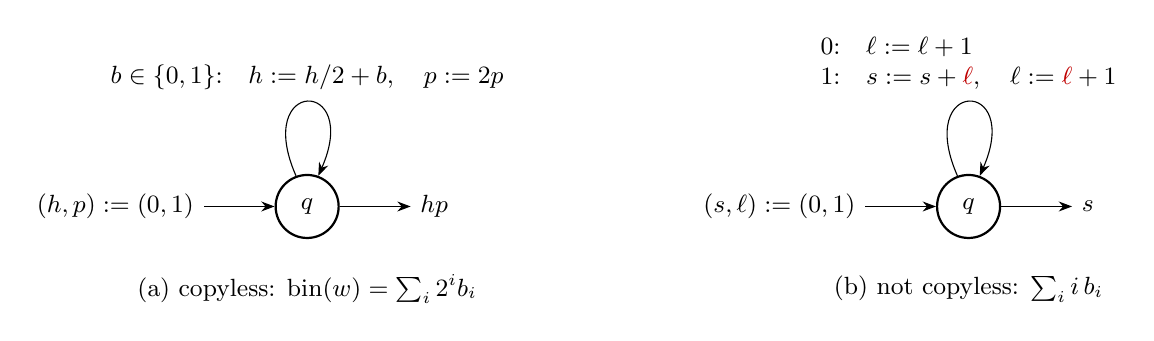
\begin{tikzpicture}[>=Stealth,font=\small,
  state/.style={draw,circle,thick,minimum size=8mm,inner sep=0pt}]
\node[state] (q) at (0,0) {$q$};
\draw[<-] (q.west) -- ++(-0.9,0) node[left] {$(h,p):=(0,1)$};
\draw[->] (q.east) -- ++(0.9,0) node[right] {$hp$};
\draw[->] (q.110) .. controls +(-0.55,1.25) and +(0.55,1.25) .. (q.70)
  node[pos=0.5,above=1pt,align=center] {$b\in\{0,1\}$:\quad $h:=h/2+b,\quad p:=2p$};
\node at (0,-1.05) {(a) copyless: $\bin(w)=\sum_i2^ib_i$};
\begin{scope}[xshift=8.4cm]
\node[state] (r) at (0,0) {$q$};
\draw[<-] (r.west) -- ++(-0.9,0) node[left] {$(s,\ell):=(0,1)$};
\draw[->] (r.east) -- ++(0.9,0) node[right] {$s$};
\draw[->] (r.110) .. controls +(-0.55,1.25) and +(0.55,1.25) .. (r.70)
  node[pos=0.5,above=1pt,align=left] {$0$:\quad $\ell:=\ell+1$\\$1$:\quad $s:=s+\textcolor{red!75!black}{\ell},\quad \ell:=\textcolor{red!75!black}{\ell}+1$};
\node at (0,-1.05) {(b) not copyless: $\sum_i i\,b_i$};
\end{scope}
\end{tikzpicture}
\caption{Initial valuations label the entry arrows and outputs label the exit arrows. (a)~Each register is updated in isolation, and the registers meet only in the output $hp$. (b)~On letter $1$ the register $\ell$ is read twice (highlighted). By Theorem~\ref{thm:sectors}(1) no CCRA computes this function, since its unipotent minimal letter matrices do not commute.}\label{fig:machine}
\end{figure}

\paragraph{Sectors and consequences.}
Two sectors give especially concrete forms. Call $f$ \emph{unipotent} (resp.\ \emph{quasi-unipotent}) if all eigenvalues of all word matrices $M_w$ of its minimal representation equal $1$ (resp.\ are roots of unity). For a morphism $\varphi:\Sigma^*\to F$ to a finite group, let $|w|_{h,a}$ count the positions $i$ of $w$ with $w_i=a$ and $\varphi(w_1\cdots w_{i-1})=h$.

\begin{theorem}[Two sectors]\label{thm:sectors}
Let $f:\Sigma^*\to\Q$ be a rational series.
\begin{enumerate}[label=(\arabic*),leftmargin=2.2em]
\item If $f$ is unipotent, then $f$ is CCRA-computable iff its minimal letter matrices commute, iff $f$ is invariant under permutations of input positions, iff $f(w)$ is a rational polynomial in the letter counts $(|w|_a)_a$.
\item If $f$ is quasi-unipotent, then $f$ is CCRA-computable iff any two word matrices $M_x,M_y$ that are unipotent commute, iff $\Gamma_f$ is virtually abelian, iff there are a finite group $F$, a morphism $\varphi:\Sigma^*\to F$ and polynomials $P_g\in\Q[n_{h,a}:h\in F,a\in\Sigma]$ with $f(w)=P_{\varphi(w)}\bigl((|w|_{h,a})_{h,a}\bigr)$ for all words $w$.
\end{enumerate}
\end{theorem}

\begin{corollary}\label{cor:consequences}
Let $f$ be invertible and CCRA-computable. Then $f$ is computed by a polynomially ambiguous weighted automaton, and its reversal $w\mapsto f(w^{\mathrm{rev}})$ is CCRA-computable. Consequently any CCRA series whose reversal is not CCRA-computable has a minimal letter matrix that is singular of rank at least two (Theorem~\ref{thm:rankone}); such series exist (Corollary~\ref{cor:reversal}). The polynomially ambiguous series of~\cite[Example~17]{MPS26} is invertible but not CCRA-computable.
\end{corollary}

Conversely, an invertible series is polynomially ambiguous iff $\cG_f^\circ$ is triangularizable over $\Q$ (Theorem~\ref{thm:polyamb}); this is an intrinsic form of the characterization of polynomial ambiguity by Puch and Smertnig~\cite{PS24}, and what is new is the condition on $\cG_f^\circ$, a direct proof and a deterministic polynomial-time test. Thus in the invertible sector CCRA-computability is exactly polynomial ambiguity plus commutation of unipotent elements, and polynomial ambiguity is decidable in deterministic polynomial time (Corollary~\ref{cor:polyamb}).

\begin{theorem}\label{thm:decision}
From a rational weighted representation one can compute its minimal representation and decide whether it is invertible in polynomial bit time. For invertible series, CCRA-computability is decidable by a Zariski-closure computation (Appendix~\ref{sec:algorithms}) and, more efficiently, as stated below. Unipotence of a series is decidable in polynomial bit time, and for unipotent series CCRA-computability is decidable in polynomial bit time. More generally, quasi-unipotence of an invertible series and, for quasi-unipotent series, CCRA-computability are decidable in deterministic polynomial bit time, and CCRA-computability of invertible series is decidable in deterministic polynomial time (Theorems~\ref{thm:polytime} and~\ref{thm:detpoly}).
\end{theorem}

Finally, the position-sum function of~\cite[Example~26]{MPS26},
\begin{equation}\label{eq:witness}
 f(b_1\cdots b_j)=\sum_{i=1}^j i\,b_i,\qquad b_i\in\{0,1\},
\end{equation}
is unipotent and not permutation-invariant, so by Theorem~\ref{thm:sectors}(1) it is not CCRA-computable. Mazowiecki, Puch and Smertnig computed that it satisfies their uniform pumping condition~\cite[Example~26]{MPS26}; Theorem~\ref{thm:pumping} records this with ring $\Z[1/2]$ and exponent $m=1$. Hence that condition is not sufficient, as conjectured in~\cite[Section~3.2]{MPS26}. The obstruction is the noncommutation of minimal unipotent matrices, a property not detected by this uniform condition.

\begin{table}[t]
\centering
\begin{tabular}{@{}>{\raggedright\arraybackslash}p{.19\linewidth}>{\raggedright\arraybackslash}p{.29\linewidth}>{\raggedright\arraybackslash}p{.27\linewidth}>{\raggedright\arraybackslash}p{.15\linewidth}@{}}
\toprule
Minimal class & CCRA criterion & Realization & Decidability\\
\midrule
Invertible & Rational triangularity of $\cG_f^\circ$; commuting unipotents & Permutation control; isolated affine registers & Deterministic polynomial time (Thm.~\ref{thm:detpoly})\\
Quasi-unipotent & $\Gamma_f$ virtually abelian & Polynomials in finite-group transition counts & Deterministic polynomial time (Thm.~\ref{thm:polytime})\\
Unipotent & Minimal letter matrices commute & Polynomials in letter counts & Polynomial bit time\\
\bottomrule
\end{tabular}
\caption{The three nested classes. The eigenvalue assumptions concern every word matrix.}\label{tab:classes}
\end{table}

\paragraph{Proof ideas.}
The central difficulty is that an invertible function may be presented by a machine with resets and nonlinear updates. We must recover reversible structure from such a presentation, without assuming that its physical updates are invertible. Figure~\ref{fig:roadmap} shows the route through both directions.

A unipotent matrix is one whose eigenvalues are all $1$; its nilpotent logarithm records additive accumulation. The component group $\cG_f/\cG_f^\circ$ is finite and records periodic behavior, such as parity, that finite control can track. Condition~(C3) constrains only the identity component. It must be triangularizable over $\Q$, and then (Lemma~\ref{lem:split}) it is a product $T\ltimes U$ of a $\Q$-split torus $T$, which scales by rational factors, and the group $U$ of its unipotent elements, which must be commutative.

The necessity direction (C1)$\Rightarrow$(C3) has three steps.
\emph{Compression.} A copyless map acts linearly, by pullback, on the $2^r$-dimensional space of multiaffine polynomials in $r$ registers. A word whose register map has the fewest nonconstant coordinates yields a copyless retraction whose pullback is a polynomial in a word operator. It therefore acts as the identity on the minimal subquotient. For a one-state machine it compresses all letters simultaneously to \emph{affine coordinate permutations} $x_i\mapsto\alpha_ix_{\pi(i)}+\beta_i$ acting on one common invariant subquotient that is isomorphic to the minimal representation (Section~\ref{sec:compression}). This step has no counterpart in pumping arguments, which constrain iterated factors one at a time: compression extracts, from an arbitrary machine with resets and products, a normal form for the action of the whole monoid at once.
\emph{Algebraic groups.} Pullbacks of affine coordinate permutations form a linear algebraic group whose identity component is triangular over $\Q$ and whose unipotent elements are pullbacks of translations, hence commute. Both properties pass to Zariski closures, images and invariant subquotients (Lemma~\ref{lem:wk} and Corollary~\ref{cor:onestate}).
\emph{Finite control.} Fix a word $t$ whose image $\delta(S,t)$ in the set $S$ of control states is as small as possible, and a power $e$ of $t$ that fixes this image pointwise. For every word $x$, a fixed power of the \emph{return block} $exe$ also fixes the image pointwise. The Zariski closure of the matrices of these words contains all $m_0$-th powers, for one fixed positive integer $m_0$, of elements of $\cG_f^\circ$, hence all of $\cG_f^\circ$, because a connected group of finite exponent is trivial. For each prefix $u$, the part of the linearized register space that is visible from the valuation reached after $ue$ is a quotient of the minimal representation (a \emph{local quotient}, Lemma~\ref{lem:local}), and finitely many local quotients jointly embed the minimal representation (Section~\ref{sec:control}).

The sufficiency direction (C3)$\Rightarrow$(C2) uses the decomposition $\cG_f^\circ=T\ltimes U$. A permutation automaton tracks the coset of the prefix in $\Gamma_f/(\Gamma_f\cap\cG_f^\circ)$. A telescoping cocycle moves the remaining dynamics into $\cG_f^\circ$. The torus contributes products of rational scalars. Because $U$ is commutative, its logarithm accumulates in isolated affine registers $z:=\chi(t)^{-1}z+\beta$ (Section~\ref{sec:normalform}).

\begin{figure}[t]
\centering
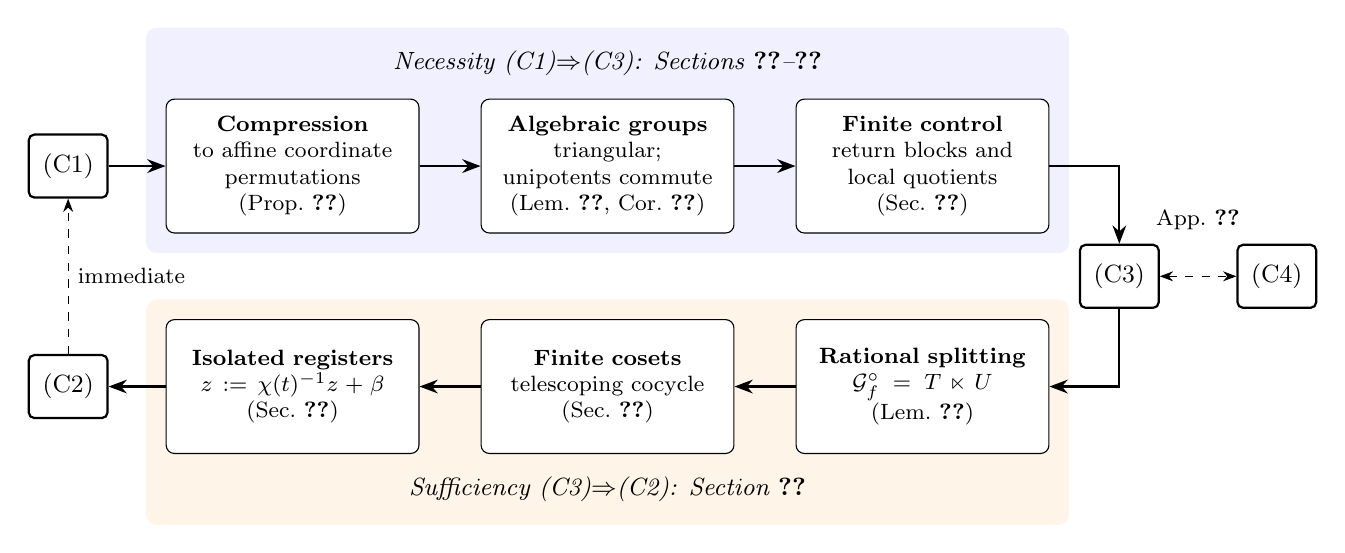
\begin{tikzpicture}[>=Stealth,font=\small,
  cond/.style={draw,thick,rounded corners=2pt,minimum width=10mm,minimum height=8mm,inner sep=2pt,fill=white},
  stp/.style={draw,rounded corners=3pt,align=center,text width=30mm,minimum height=17mm,inner sep=3pt,fill=white,font=\footnotesize},
  lab/.style={font=\small\itshape,inner sep=1pt}]
\node[cond] (c1) at (0,0) {(C1)};
\node[cond] (c2) at (0,-2.8) {(C2)};
\node[stp] (s1) at (2.85,0) {\textbf{Compression}\\to affine coordinate\\permutations\\(Prop.~\ref{prop:compression})};
\node[stp] (s2) at (6.85,0) {\textbf{Algebraic groups}\\triangular;\\unipotents commute\\(Lem.~\ref{lem:wk}, Cor.~\ref{cor:onestate})};
\node[stp] (s3) at (10.85,0) {\textbf{Finite control}\\return blocks and\\local quotients\\(Sec.~\ref{sec:control})};
\node[stp] (s4) at (10.85,-2.8) {\textbf{Rational splitting}\\$\cG_f^\circ=T\ltimes U$\\(Lem.~\ref{lem:split})};
\node[stp] (s5) at (6.85,-2.8) {\textbf{Finite cosets}\\telescoping cocycle\\(Sec.~\ref{sec:normalform})};
\node[stp] (s6) at (2.85,-2.8) {\textbf{Isolated registers}\\$z:=\chi(t)^{-1}z+\beta$\\(Sec.~\ref{sec:normalform})};
\node[cond] (c3) at (13.35,-1.4) {(C3)};
\node[cond] (c4) at (15.35,-1.4) {(C4)};
\node[lab,above=2.5mm of s2] (nl) {Necessity (C1)$\Rightarrow$(C3): Sections~\ref{sec:compression}--\ref{sec:control}};
\node[lab,below=2.5mm of s5] (sl) {Sufficiency (C3)$\Rightarrow$(C2): Section~\ref{sec:normalform}};
\begin{scope}[on background layer]
\node[fill=blue!6,rounded corners=4pt,inner sep=2.5mm,fit=(s1)(s2)(s3)(nl)] {};
\node[fill=orange!9,rounded corners=4pt,inner sep=2.5mm,fit=(s4)(s5)(s6)(sl)] {};
\end{scope}
\draw[->,thick] (c1)--(s1);\draw[->,thick] (s1)--(s2);\draw[->,thick] (s2)--(s3);
\draw[->,thick] (s3.east) -| (c3.north);
\draw[->,thick] (c3.south) |- (s4.east);
\draw[->,thick] (s4)--(s5);\draw[->,thick] (s5)--(s6);\draw[->,thick] (s6)--(c2);
\draw[->,dashed] (c2)--node[right,font=\footnotesize]{immediate}(c1);
\draw[<->,dashed] (c3)--(c4);
\path (c3.north) -- node[above=0.5mm,font=\footnotesize]{App.~\ref{sec:sectors}} (c4.north);
\end{tikzpicture}
\caption{Proof route. Top: necessity recovers algebraic-group constraints from an arbitrary CCRA. Bottom: sufficiency builds the normal form. Dashed: (C2)$\Rightarrow$(C1) is immediate, and (C3)$\Leftrightarrow$(C4) is proved in Appendix~\ref{sec:sectors}.}\label{fig:roadmap}
\end{figure}

\paragraph{Related work.}
Mazowiecki and Riveros~\cite{MR16,MR19} developed the structure theory of CCRA over semirings, including a syntactic normal form using register permutations in finite control and an analysis of stable registers and resets. Their nonvanishing affine-growth conclusions additionally require a nonzero semiring and a nonzero automaton; those assumptions fail for signed rationals with cancellation. Their reversal counterexample is over the max-plus semiring. Our normal form~(C2) is much stronger in the invertible sector. The pumping theory of~\cite{MPS26} is the direct starting point. The squarefree linearization is folklore~\cite[Lemma~50]{MPSfull}. Puch and Smertnig~\cite{PS24} characterize, for invertible weighted automata, finite and polynomial ambiguity by arithmetic conditions, using unit equations and monomial covers, and obtain decidability via Zariski closures~\cite{DJK05,NPSSW22}. Our decision procedure of Appendix~\ref{sec:algorithms} follows the same pattern, while Appendix~\ref{sec:polytime} gives a closure-free procedure; the property and the proof are different. Theorem~\ref{thm:polyamb} recasts their characterization of polynomial ambiguity intrinsically, in terms of $\cG_f^\circ$, as triangularizability of $\cG_f^\circ$ over $\Q$, with a direct proof and a deterministic polynomial-time test, and shows that the invertible CCRA series are exactly the polynomially ambiguous ones with commutative unipotent radical. Bell and Smertnig characterized unambiguous series~\cite{BS21} and decided whether a series is computed by a deterministic, respectively unambiguous, weighted automaton~\cite{BS23}, and Jecker, Mazowiecki and Purser~\cite{JMP24} study determinisation and unambiguisation of polynomially ambiguous rational weighted automata. Weber and Seidl~\cite{WS91} characterize polynomial ambiguity of an automaton, as opposed to a series. Kiefer, Murawski, Ouaknine, Wachter and Worrell~\cite{KMOWW13} analyse equivalence and minimisation of $\Q$-weighted automata, and Zariski closures of matrix monoids also underlie the computation of polynomial invariants of affine programs~\cite{HOPW18}. Pumping lemmas for weighted automata were developed by Chattopadhyay, Mazowiecki, Muscholl and Riveros~\cite{CMMR21}, and Daviaud, Reynier and Talbot~\cite{DRT16} minimise cost register automata. Clemente~\cite{C25,clemente:LIPIcs.LICS.2026.29} studies commutativity problems and commutative products of series, and Benalioua, Lhote and Reynier~\cite{benalioua_et_al:LIPIcs.MFCS.2024.23} minimize linear and affine CRA; neither addresses the existence of copyless realizations. Douéneau-Tabot~\cite{doueneautabot:LIPIcs.ICALP.2022.120} characterizes the unary-output functions of pebble and blind transducers through $\N$-rational series and their Cauchy and Hadamard products, and decides whether a given pebble transducer defines a blind function; there outputs are natural numbers and the machines are two-way.

\paragraph{Organization.}
Section~\ref{sec:prelim} fixes models and algebraic-group tools. Section~\ref{sec:compression} proves the compression theorem for monoids of copyless maps, Section~\ref{sec:control} handles finite control and proves (C1)$\Rightarrow$(C3), and Section~\ref{sec:normalform} proves (C3)$\Rightarrow$(C2). Appendix~\ref{sec:sectors} proves (C3)$\Leftrightarrow$(C4) and Theorem~\ref{thm:sectors}. Appendix~\ref{sec:consequences} proves Corollary~\ref{cor:consequences}, discusses examples, establishes the pumping property of~\eqref{eq:witness}, and characterizes polynomial ambiguity in the invertible sector (Appendix~\ref{ssec:polyamb}). Appendix~\ref{sec:algorithms} proves the first claims of Theorem~\ref{thm:decision} and gives polynomial-size synthesis and short certificates for explicit pattern sums. Appendix~\ref{sec:polytime} gives the polynomial-time decision procedures, proves that they run in deterministic polynomial time, and proves the remaining claims. Appendix~\ref{sec:singular} treats singular series: rank-one resets, the inverse-weight and lifting obstructions, non-closure under reversal, and an exact characterization for one invertible letter and one rank-two reset. Appendix~\ref{sec:singular} opens with a local necessary condition for singular series (Corollary~\ref{cor:local}), and Appendix~\ref{sec:open} discusses the limits of the characterization and open problems. The proof of Theorem~\ref{thm:main} uses only Sections~\ref{sec:prelim}--\ref{sec:normalform} and Appendix~\ref{sec:sectors}; decidability, the polynomial-time algorithm in the quasi-unipotent sector and the Monte Carlo algorithm do not depend on the height bound of Appendix~\ref{ssec:detpoly}. The AI methodology statement precedes the references.

\section{Models, representations and algebraic groups}\label{sec:prelim}
\subsection{Copyless machines and their linearization}
A polynomial expression is \emph{copyless} if each variable occurs at most once in it. A tuple of expressions is copyless if each variable occurs at most once across the entire tuple. Consequently its coordinate polynomials are multiaffine (of degree at most one in each variable) and distinct coordinates have disjoint variable supports; cancellation can remove variables but does not invalidate these conclusions. Compositions of copyless tuples are copyless.

A deterministic copyless polynomial cost register automaton (CCRA) over $\Q$ consists of a finite set $S$ of control states with initial state $s_0$, a complete deterministic transition function $\delta:S\times\Sigma\to S$, registers $x_1,\ldots,x_r$ with an initial valuation $x^{(0)}\in\Q^r$, a copyless polynomial update $P_{s,a}:\Q^r\to\Q^r$ for every transition, and a copyless output polynomial $\omega_s$ for every state; all constants are rational. Extend $\delta$ to words, and let $P_{s,z}$ be the composite update along the run of $z$ from $s$, so $P_{s,zz'}=P_{\delta(s,z),z'}\circ P_{s,z}$. The machine computes $f(w)=\omega_{\delta(s_0,w)}\bigl(P_{s_0,w}(x^{(0)})\bigr)$. A \emph{permutation automaton} is a control in which every letter permutes $S$.

Let $V_r$ be the space of multiaffine polynomials in $x_1,\ldots,x_r$, with basis the squarefree monomials $x_I=\prod_{i\in I}x_i$, $I\subseteq\{1,\ldots,r\}$. For a copyless map $P$, the pullback $B_P(h)=h\circ P$ preserves $V_r$, because substituting into a squarefree monomial multiplies polynomials with disjoint supports. Thus $B_{P\circ P'}=B_{P'}B_P$, and every CCRA computes a rational series: on $\bigoplus_{s\in S}V_r$ let $(B_ah)_s=h_{\delta(s,a)}\circ P_{s,a}$, let $\lambda(h)=h_{s_0}(x^{(0)})$ and $o=(\omega_s)_s$; then $f(w)=\lambda B_{a_1}\cdots B_{a_n}o$.

\subsection{Weighted representations}
A representation of $f$ is a triple of a row vector $\lambda$, matrices $M_a$ and a column vector $\gamma$ with $f(w)=\lambda M_w\gamma$. It is minimal if the row vectors $\lambda M_w$ span the dual space and the columns $M_w\gamma$ span the space. Minimal representations exist, are computable, and are unique up to simultaneous conjugation~\cite{Sch61,BR11}. More precisely, for an arbitrary representation on a space $X$ put
\begin{equation}\label{eq:WN}
W=\spn\{M_w\gamma:w\in\Sigma^*\},\qquad N=\{h\in W:\lambda M_vh=0\text{ for all }v\in\Sigma^*\}.
\end{equation}
Both are invariant, and the map $W\to\Q^{\Sigma^*}$, $h\mapsto(v\mapsto\lambda M_vh)$, has kernel $N$ and sends $M_w\gamma$ to the residual $v\mapsto f(vw)$. Hence the induced representation on $W/N$ is isomorphic to every minimal representation. In particular, \emph{the minimal representation is an invariant subquotient of every representation}, and if all $M_a$ are invertible then so are the minimal letter matrices.

\subsection{Algebraic-group tools}
For a group $\Gamma\le\GL_d(\Q)$ its Zariski closure $\cG\subseteq\GL_d(\Qb)$ is the set of common zeros in $\GL_d(\Qb)$ of all polynomials in the entries and $\det^{-1}$ that vanish on $\Gamma$. It is a linear algebraic group defined over $\Q$. We use the following standard facts~\cite{Bor91,Hum75}.
\begin{enumerate}
\item[(A1)] $\cG$ has a connected normal closed subgroup $\cG^\circ$ of finite index, whose cosets are the irreducible components of $\cG$; every closed subgroup of finite index contains $\cG^\circ$.
\item[(A2)] Every $g\in\cG$ has a Jordan decomposition $g=g_sg_u=g_ug_s$ with $g_s$ semisimple, $g_u$ unipotent, and $g_s,g_u\in\cG$. For $g\in\GL_d(\Q)$ both factors are polynomials in $g$ with rational coefficients. Morphisms of algebraic groups preserve Jordan decompositions. Images of algebraic groups under morphisms are closed, and the image of the identity component is the identity component of the image.
\item[(A3)] In characteristic zero every unipotent element of $\cG$ lies in $\cG^\circ$: if $u\ne1$ is unipotent, the closure of $\langle u\rangle$ is the irreducible curve $\{\exp(t\log u)\}$.
\item[(A4)] A connected algebraic group all of whose elements are semisimple is a torus~\cite{Bor91}. A connected group whose maximal tori are trivial is unipotent, since each element lies in a Borel subgroup $B=T_BB_u$ with $T_B$ a maximal torus~\cite{Bor91}. In characteristic zero, a connected group of finite exponent is trivial: unipotent elements of finite order are trivial, so all elements are semisimple, and a torus of finite exponent is trivial.
\item[(A5)] For connected $H$, a subspace is $H$-invariant iff it is invariant under the Lie algebra of $H$~\cite{Hum75}. Indeed, the stabilizer of the subspace is closed; its Lie algebra contains $\operatorname{Lie}(H)$, so in characteristic zero its intersection with connected $H$ has full dimension and equals $H$.
\end{enumerate}
\begin{lemma}[Rational splitting and weights]\label{lem:split}
Let $H\le\GL_d$ be connected, defined over $\Q$, and triangularizable over $\Q$. Its unipotent elements form its connected unipotent radical $U$, defined over $\Q$. There is a split torus $T$ defined over $\Q$ such that multiplication $T\times U\to H$ is an isomorphism of varieties. In particular $H(\Q)=T(\Q)U(\Q)$. Every rational representation of $T$, including its conjugation action on $\operatorname{Lie}(U)$, decomposes into rational weight spaces.
\end{lemma}
\begin{proof}
Choose a rational basis making $H$ upper triangular. The diagonal map has unipotent kernel; for connected solvable groups that kernel is the unipotent radical, and the maximal-torus decomposition over a perfect field gives a torus $T$ defined over $\Q$ with $H=T U$ and $T\cap U=1$~\cite[Theorems~10.6(1),(4) and~18.2(i)]{Bor91}. These structural results give the multiplication isomorphism over $\Q$. The diagonal map restricted to $T$ has trivial kernel, since a torus has no nonidentity unipotent element. In characteristic zero its image is a closed subtorus and this map identifies $T$ with a subtorus of the split diagonal torus. Such a subtorus is split: its character group is a quotient of the diagonal torus's character group and has trivial Galois action. Thus all characters and their weight spaces in rational representations are defined over $\Q$~\cite[\S8]{Bor91}.

For completeness, if $h\in H(\Q)$ write its unique decomposition as $h=tu$ over $\Qb$. Every Galois automorphism fixes $h$ and preserves $T$ and $U$. Uniqueness gives $\sigma(t)=t$ and $\sigma(u)=u$, so $t\in T(\Q)$ and $u\in U(\Q)$. The conjugation representation on the rational invariant space $\operatorname{Lie}(U)$ is a rational representation of this split torus, so the same weight-space conclusion applies to it.
\end{proof}

For a unipotent rational matrix $u$, $\log u=\sum_{j\ge1}(-1)^{j+1}(u-I)^j/j$ is a rational nilpotent matrix; $\exp$ and $\log$ are inverse bijections between unipotent and nilpotent matrices, and $\exp(X+Y)=\exp X\exp Y$ when $X,Y$ commute.

\begin{lemma}\label{lem:monoid}
Let $S\subseteq\GL_d(\Q)$ be a submonoid generating the group $\Gamma$, with Zariski closure $\cG$ of $\Gamma$. Then $S$ is Zariski dense in $\cG$, and $S\cap\cG^\circ$ is Zariski dense in $\cG^\circ$. The same holds for $\Gamma$, and $\Gamma\cap\cG^\circ$ is a normal subgroup of finite index in $\Gamma$.
\end{lemma}
\begin{proof}
Let $\bar S$ be the closure of $S$. Right multiplication by $s\in S$ is a homeomorphism mapping $S$ into $S$, so $\bar Ss\subseteq\bar S$. Hence for $x\in\bar S$ the closed set $\{y:xy\in\bar S\}$ contains $S$, hence $\bar S$; so $\bar S$ is a monoid. For $x\in\bar S$ the descending chain $\bar S\supseteq x\bar S\supseteq x^2\bar S\supseteq\cdots$ of closed sets stabilizes, and cancelling a power of $x$ gives $\bar S=x\bar S$, so $x^{-1}\in\bar S$. Thus $\bar S$ is a closed group containing $\Gamma$, and $\bar S=\cG$. As $\cG$ is the finite disjoint union of the closed cosets $g\cG^\circ$, we have $\cG=\bigcup_g\overline{S\cap g\cG^\circ}$ with $\overline{S\cap g\cG^\circ}\subseteq g\cG^\circ$; intersecting with $\cG^\circ$ gives $\overline{S\cap\cG^\circ}=\cG^\circ$. The last claim follows from (A1).
\end{proof}

\begin{lemma}\label{lem:root}
If $u$ is a unipotent $d\times d$ rational matrix and $t\ge1$, then
\[
u=\sum_{j=0}^{d-1}\binom{1/t}{j}(u^t-I)^j.
\] In particular $u$ commutes with every matrix commuting with $u^t$, and $g_u$ commutes with every matrix commuting with $(g^t)_u=(g_u)^t$.
\end{lemma}
\begin{proof}
In $\Q[X]/(X^d)$ substitute $Y=(1+X)^t-1$ into the truncated series $(1+Y)^{1/t}=1+X$, and put $X=u-I$. The second statement applies this to $g_u$, using $(g^t)_u=(g_u)^t$.
\end{proof}

\section{Compression of a monoid of copyless maps}\label{sec:compression}
Throughout this section, $\cY$ is a monoid acting on $\Q^r$ by copyless polynomial maps $P_y$ with $P_1=\id$ and $P_{yz}=P_z\circ P_y$. Its pullbacks $B_y=B_{P_y}$ on $V_r$ satisfy $B_{yz}=B_yB_z$. We fix subspaces $N\subseteq W\subseteq V_r$ invariant under every $B_y$, write $D=W/N$, and let $\rho(y)$ be the operator induced by $B_y$ on $D$. In Section~\ref{sec:control} the monoid $\cY$ will consist of return words of a CCRA.

For a copyless map $P:\Q^r\to\Q^r$ let $k(P)$ be the number of nonconstant coordinates of $P$, let $L_P$ be the coordinate affine subspace obtained by fixing each constant coordinate to its value, and let $V(L_P)$ be the multiaffine polynomials in its $k(P)$ free coordinates.

\begin{lemma}\label{lem:image}
$P$ maps $\Q^r$ onto $L_P(\Q)$, $\operatorname{rank}B_P=2^{k(P)}$, and $\ker B_P=\{h\in V_r:h|_{L_P}=0\}$.
\end{lemma}
\begin{proof}
A nonconstant multiaffine $q$ over $\Q$ is onto $\Q$: write $q=x_ia+b$ with $a\ne0$ free of $x_i$, specialize the other variables to rationals where $a\ne0$ (possible since a nonzero polynomial over an infinite field does not vanish on all rational points), and solve for $x_i$. Distinct nonconstant coordinates of $P$ have disjoint supports, so these choices are independent; this gives surjectivity. Restriction $V_r\to V(L_P)$ is onto, and pullback $V(L_P)\to V_r$ through $P$ is injective because $P$ is onto $L_P(\Q)$. Factoring $B_P$ through these maps proves the remaining claims.
\end{proof}

Choose $\eta\in\cY$ minimizing $k(P_{\eta})$ and put $P=P_{\eta}$, $k=k(P)$, $L=L_P$. The element $\eta\eta$ has at most $k$ nonconstant coordinates, hence exactly $k$; as $P$ is onto $L$, all $k$ free coordinates of $A=P|_L:L\to L$ are nonconstant. Restriction preserves disjointness of supports, so each free output of $A$ uses exactly one free variable and all are used. By multiaffinity,
\begin{equation}\label{eq:affineperm}
 A_i(t)=\alpha_it_{\pi(i)}+\beta_i,\qquad\alpha_i\in\Q^\times,
\end{equation}
for a permutation $\pi$. We call such a map an \emph{affine coordinate permutation}. Define the copyless retraction $Q=A^{-1}\circ P:\Q^r\to L$. It is onto $L$ and $Q|_L=\id_L$, so $E=B_Q$ is idempotent.

\begin{lemma}\label{lem:projection}
$E$ is the projection onto $\im B_{\eta}$ along $\ker B_{\eta}$, and $E=p(B_{\eta})$ for some $p\in\Q[T]$.
\end{lemma}
\begin{proof}
Composition with $A^{-1}$ is an automorphism of $V(L)$, so $\im B_Q=\im B_P$; both maps are onto $L$, so Lemma~\ref{lem:image} gives $\ker B_Q=\ker B_P$. Since $k(P_{\eta\eta})=k(P_{\eta})$, $\operatorname{rank}B_{\eta}^2=\operatorname{rank}B_{\eta}$, hence $V_r=\ker B_{\eta}\oplus\im B_{\eta}$ and $B_{\eta}$ is invertible on its image. If $q$ is the minimal polynomial of $B_{\eta}|_{\im B_{\eta}}$, then $q(0)\ne0$, and the Chinese remainder theorem gives $p\in\Q[T]$ with $p\equiv0\bmod T$ and $p\equiv1\bmod q$. Then $p(B_{\eta})$ vanishes on $\ker B_{\eta}$ and is the identity on $\im B_{\eta}$.
\end{proof}

\begin{proposition}[Compression]\label{prop:compression}
Assume that $\rho(y)$ is invertible for every $y\in\cY$. Then there are $k\ge0$, affine coordinate permutations $R_y$ of $\Q^k$ $(y\in\cY)$, and subspaces $N''\subseteq W''\subseteq V_k$ invariant under every pullback $B_{R_y}$, together with a linear isomorphism $W''/N''\cong D$ intertwining the operator induced by $B_{R_y}$ with $\rho(y)$ for every $y$.
\end{proposition}
\begin{proof}
By Lemma~\ref{lem:projection}, $E$ preserves $W$ and $N$; let $\bar E$ be its induced operator on $D$. Since $\im B_{\eta}=\im E$, we have $(I-E)B_{\eta}=0$, so $(I-\bar E)\rho(\eta)=0$, and invertibility of $\rho(\eta)$ gives $\bar E=I$, that is, $(I-E)W\subseteq N$, although the physical map $P_{\eta}$ need not be invertible.

Let $J:V(L)\to\im E$, $J(h)=h\circ Q$, with inverse $g\mapsto g|_L$, and put $R_y=Q\circ P_y|_L:L\to L$ and $C_y=EB_yE$. Direct substitution gives $C_yJ(h)=h\circ Q\circ P_y\circ Q=J(B_{R_y}h)$. Each $R_y$ is copyless. The register map of $\eta y\eta$ is $P_{\eta}\circ P_y\circ P_{\eta}=A\circ R_y\circ(A\circ Q)$, where $A\circ Q=P_{\eta}$ is onto $L$ and $A$ rescales and translates free coordinates. Hence $P_{\eta y\eta}$ has as many nonconstant coordinates as $R_y$ has nonconstant free outputs, and minimality of $\eta$ forces $k$ of them; the support count used for~\eqref{eq:affineperm} shows that $R_y$ is an affine coordinate permutation.

Put $W'=EW\subseteq W$ and $N'=W'\cap N$. Both are invariant under every $C_y$, because $E$ and $B_y$ preserve $W$ and $N$ and $E$ is the identity on $W'$. The map $W'/N'\to W/N$, $h+N'\mapsto h+N$, is injective by definition of $N'$ and surjective because $h-Eh\in N$ for $h\in W$. For $h\in W'$ we have $C_yh-B_yh=(E-I)B_yh\in N$, so the map intertwines $C_y$ with $\rho(y)$. Finally set $W''=J^{-1}W'$ and $N''=J^{-1}N'$. If $k=0$, all objects are at most one-dimensional and the statement is trivial.
\end{proof}
The assignment $y\mapsto R_y$ need not be multiplicative; only the induced operators on $W''/N''$ form a representation of $\cY$, which is the action needed in the next corollary.

Let $\mathfrak A_k$ be the algebraic group of affine coordinate permutations of affine $k$-space over $\Qb$, that is, $(\Qb^\times\ltimes\Qb)^k\rtimes S_k$, and let $\cW_k=\{B_R:R\in\mathfrak A_k\}\subseteq\GL(V_k\otimes\Qb)$.

\begin{lemma}\label{lem:wk}
$\cW_k$ is a closed subgroup. Its identity component consists of the pullbacks of the maps $x\mapsto(\alpha_ix_i+\beta_i)_i$; it preserves the complete rational flag spanned by the squarefree monomials taken in order of nondecreasing degree. The unipotent elements of $\cW_k$ are exactly the pullbacks of translations; in particular they commute pairwise.
\end{lemma}
\begin{proof}
$R\mapsto B_R$ is an anti-homomorphism of algebraic groups, so its image is closed (A2), and its identity component is the image of the connected finite-index subgroup $(\Qb^\times\ltimes\Qb)^k$. For $R(x)=(\alpha_ix_i+\beta_i)_i$ we have $B_Rx_I=\prod_{i\in I}(\alpha_ix_i+\beta_i)=(\prod_{i\in I}\alpha_i)x_I+\sum_{I'\subsetneq I}c_{I'}x_{I'}$, which gives the triangular form with diagonal entries $\prod_{i\in I}\alpha_i$. Such $B_R$ is unipotent iff $\alpha_i=1$ for all $i$ (take $I=\{i\}$), that is, iff $R$ is a translation. Every unipotent element of $\cW_k$ lies in $\cW_k^\circ$ by (A3). Translations commute, and so do their pullbacks.
\end{proof}

\begin{corollary}[One-state constraint]\label{cor:onestate}
Under the hypothesis of Proposition~\ref{prop:compression}, let $\cH$ be the Zariski closure of $\{\rho(y):y\in\cY\}$ in $\GL(D)$. Then any two unipotent elements of $\cH$ commute, and $\cH^\circ$ is triangularizable over $\Q$.
\end{corollary}
\begin{proof}
By Lemma~\ref{lem:monoid}, $\cH$ is a group. Let $\mathcal S\subseteq\GL(V_k\otimes\Qb)$ be the closed subgroup stabilizing $W''$ and $N''$, and let $\pi:\mathcal S\to\GL(W''/N'')\cong\GL(D)$ be the induced-action morphism. Let $\cG_L$ be the Zariski closure of the group generated by the $B_{R_y}$; it lies in $\cW_k\cap\mathcal S$. By (A2), $\pi(\cG_L)$ is closed; it contains every $\rho(y)$ and is contained in the closure of the group they generate, so $\pi(\cG_L)=\cH$. If $h\in\cH$ is unipotent, write $h=\pi(g)$ with $g\in\cG_L$; then $h=h_u=\pi(g_u)$ with $g_u\in\cG_L$ unipotent, hence the pullback of a translation by Lemma~\ref{lem:wk}. Two such elements commute, and so do their images. Moreover $\cH^\circ=\pi(\cG_L^\circ)$ with $\cG_L^\circ\subseteq\cW_k^\circ$, which preserves the rational monomial flag of Lemma~\ref{lem:wk}; its traces on $W''$ modulo $N''$ form a chain of rational $\cH^\circ$-invariant subspaces with successive quotients of dimension at most one.
\end{proof}

\section{Finite control: proof of (C1)\texorpdfstring{$\Rightarrow$}{=>}(C3)}\label{sec:control}
Fix a CCRA $\mathcal C$ as in Section~\ref{sec:prelim} computing an invertible $f$, with minimal representation $(\lambda,(M_a)_a,\gamma)$ of dimension $d\ge1$ (the case $f=0$ is trivial). Write $\cG=\cG_f$.

Words act on the finite set $S$ of control states. Choose a word $t$ for which the image ${S_{\mathrm{ret}}}=\delta(S,t)$ has minimum size. Since $\delta(S,tt)=\delta({S_{\mathrm{ret}}},t)$ cannot be smaller, $t$ permutes ${S_{\mathrm{ret}}}$. Let $m_0=|{S_{\mathrm{ret}}}|!$ and put $e=t^{m_0}$. Then $\delta(S,e)={S_{\mathrm{ret}}}$ and $e$ fixes every state of ${S_{\mathrm{ret}}}$.

\begin{lemma}\label{lem:return}
For every word $x$, the word $exe$ permutes ${S_{\mathrm{ret}}}$, and $(exe)^{m_0}$ fixes every state of ${S_{\mathrm{ret}}}$.
\end{lemma}
\begin{proof}
$\delta(S,exe)\subseteq\delta(S,e)={S_{\mathrm{ret}}}$ and minimality force equality. Since $e$ maps $S$ onto ${S_{\mathrm{ret}}}$ and fixes ${S_{\mathrm{ret}}}$, $\delta(S,exe)$ is the image of ${S_{\mathrm{ret}}}$ under $exe$; thus $exe$ maps ${S_{\mathrm{ret}}}$ onto itself, and its order as a permutation divides $|{S_{\mathrm{ret}}}|!$, which divides $m_0$.
\end{proof}

Let $L_{S_{\mathrm{ret}}}=\{z\in\Sigma^*:\delta(r,z)=r\text{ for all }r\in {S_{\mathrm{ret}}}\}$, a monoid containing $e$ and every $(exe)^{m_0}$. Let $\cK$ be the Zariski closure of $\{M_z:z\in L_{S_{\mathrm{ret}}}\}$, a closed subgroup of $\cG$ by Lemma~\ref{lem:monoid}, and let $\cA_{S_{\mathrm{ret}}}=\spn\{M_z:z\in L_{S_{\mathrm{ret}}}\}$, a unital algebra. By Cayley--Hamilton, $M_e^{-1}$ is a polynomial in $M_e$, so $M_e^{-1}\in\cA_{S_{\mathrm{ret}}}$.

\begin{lemma}\label{lem:dense}
$\cK\supseteq\cG^\circ$.
\end{lemma}
\begin{proof}
Let $g=M_e\in\cG$ and $\Phi:\cG\to\cG$, $\Phi(h)=(ghg)^{m_0}$. Then $\Phi(M_x)=M_{(exe)^{m_0}}\in\cK$ for every word $x$. As $\Phi$ is continuous and the word matrices are dense in $\cG$ (Lemma~\ref{lem:monoid}), $\Phi(\cG)\subseteq\cK$. For $k\in\cG^\circ$ we have $g^{-1}kg^{-1}\in\cG$ and $\Phi(g^{-1}kg^{-1})=k^{m_0}$; hence $\cK$ contains every $m_0$-th power of an element of $\cG^\circ$. Let $\cH$ be the closure of the group generated by these powers. It is a closed subgroup of $\cK\cap\cG^\circ$, normal in $\cG^\circ$ because its generating set is conjugation invariant. The quotient $\cG^\circ/\cH$ is a connected algebraic group of exponent dividing $m_0$, hence trivial by (A4). Thus $\cG^\circ=\cH\subseteq\cK$.
\end{proof}

\begin{lemma}[Local quotients]\label{lem:local}
Let $u\in\Sigma^*$, $q=\delta(s_0,ue)\in {S_{\mathrm{ret}}}$, and let $x_u=P_{s_0,ue}(x^{(0)})$ be the valuation after $ue$. Let $L_{S_{\mathrm{ret}}}$ act on $\Q^r$ by $P_z=P_{q,z}$, and for $s\in\Sigma^*$ let $o_s=\omega_{\delta(q,s)}\circ P_{q,s}\in V_r$. Put
\[
\begin{aligned}
W&=\spn\{o_s:s\in\Sigma^*\},\\
N&=\{h\in W:(B_zh)(x_u)=0\ \forall z\in L_{S_{\mathrm{ret}}}\},\\
K_u&=\{v\in\Q^d:\lambda M_{ue}M_zv=0\ \forall z\in L_{S_{\mathrm{ret}}}\}.
\end{aligned}
\]
Then $W$ and $N$ are invariant under every $B_z$, $K_u$ is $\cK$-invariant, and $\sum_sc_so_s\mapsto\sum_sc_sM_s\gamma+K_u$ induces a linear isomorphism $W/N\cong\Q^d/K_u$ intertwining $B_z$ with the operator induced by $M_z$, for every $z\in L_{S_{\mathrm{ret}}}$.
\end{lemma}
\begin{proof}
Since $z\in L_{S_{\mathrm{ret}}}$ returns to $q$, $P_{zz'}=P_{z'}\circ P_z$ and $B_zo_s=o_s\circ P_{q,z}=o_{zs}$; so $W$ is invariant, and so is $N$. Evaluating, $(B_zo_s)(x_u)=o_{zs}(x_u)=f(uezs)=\lambda M_{ue}M_zM_s\gamma$. If $h=\sum c_so_s$, then $(B_zh)(x_u)=\lambda M_{ue}M_z(\sum c_sM_s\gamma)$ for all $z$. Hence the map is well defined (if $h=0$ then $\sum c_sM_s\gamma\in K_u$) and its kernel is exactly $N$. It is onto because the $M_s\gamma$ span $\Q^d$, and it intertwines because $B_zo_s=o_{zs}\mapsto M_zM_s\gamma$. Finally $K_u$ is invariant under each $M_z$, $z\in L_{S_{\mathrm{ret}}}$, hence under the closure $\cK$.
\end{proof}

\begin{proof}[Proof of (C1)$\Rightarrow$(C3)]
Fix $u$. Each $M_z$ is invertible, so its induced operator on $\Q^d/K_u$ is invertible. By Lemma~\ref{lem:local}, Proposition~\ref{prop:compression} and Corollary~\ref{cor:onestate} apply to the monoid $L_{S_{\mathrm{ret}}}$ acting by $P_{q,z}$. Thus the Zariski closure $\cH_u$ of the induced operators on $\Q^d/K_u$ has pairwise commuting unipotent elements and $\cH_u^\circ$ is triangularizable over $\Q$. The restriction morphism $\res_u$ from the stabilizer of $K_u$ to $\GL(\Q^d/K_u)$ maps $\cK$ onto $\cH_u$ by (A2).

\emph{Commutation.} Let $g_1,g_2\in\cG$ be unipotent. By (A3) and Lemma~\ref{lem:dense} they lie in $\cG^\circ\subseteq\cK$, and $\res_u(g_1),\res_u(g_2)$ are unipotent elements of $\cH_u$, hence commute. So $[g_1,g_2]=g_1g_2-g_2g_1$ maps $\Q^d$ into $K_u$, that is, $\lambda M_{ue}a[g_1,g_2]=0$ for every $a\in\cA_{S_{\mathrm{ret}}}$. Taking $a=M_e^{-1}$ gives $\lambda M_u[g_1,g_2]=0$. Since $u$ is arbitrary and the $\lambda M_u$ span the dual space, $[g_1,g_2]=0$.

\emph{Triangularizability.} Taking $a=M_e^{-1}$ also shows $K_u\subseteq\ker(\lambda M_u)$, so $\bigcap_uK_u=0$, and some finite set $U_0$ of words satisfies $\bigcap_{u\in U_0}K_u=0$. The group $\cG^\circ\subseteq\cK$ preserves each $K_u$, and $\res_u(\cG^\circ)$ is connected, hence contained in $\cH_u^\circ$, which preserves a complete rational flag of $\Q^d/K_u$. The diagonal map $\Q^d\to\bigoplus_{u\in U_0}\Q^d/K_u$ is injective and $\cG^\circ$-equivariant. Concatenating the flags gives a $\cG^\circ$-invariant chain of rational subspaces of the direct sum with successive quotients of dimension at most one; intersecting it with the image of $\Q^d$ gives a complete $\cG^\circ$-invariant rational flag of $\Q^d$.
\end{proof}

The role of minimal invertibility is now explicit: it makes the compressed projection act as the identity and lets return-block operators be cancelled on the minimal state space. The register maps themselves can still discard values or multiply registers.

\section{The normal form: proof of (C3)\texorpdfstring{$\Rightarrow$}{=>}(C2)}\label{sec:normalform}
Assume~(C3) and write $\Gamma=\Gamma_f$, $\cG=\cG_f$. By Lemma~\ref{lem:monoid}, $\Gamma^\circ=\Gamma\cap\cG^\circ$ is a normal subgroup of finite index; let $F=\Gamma/\Gamma^\circ$ and $\varphi:\Sigma^*\to F$, $\varphi(w)=M_w\Gamma^\circ$. The image $\varphi(\Sigma^*)$ is a submonoid of a finite group containing the images of the generators of $\Gamma$, hence equals $F$. Choose words $r_g$ with $\varphi(r_g)=g$ and $r_1=\eps$, and put
\[
c(g,a)=M_{r_g}M_aM_{r_{g\varphi(a)}}^{-1}\in\Gamma^\circ\qquad(g\in F,\ a\in\Sigma).
\]
For $w=a_1\cdots a_n$ let $g_0=1$ and $g_i=\varphi(a_1\cdots a_i)$. Telescoping gives
\begin{equation}\label{eq:cocycle}
M_w=c(g_0,a_1)c(g_1,a_2)\cdots c(g_{n-1},a_n)M_{r_{g_n}}.
\end{equation}

By~(C3) and Lemma~\ref{lem:split}, $\cG^\circ=T\ltimes U$, where $T$ is a torus diagonalizable over $\Q$, $U$ is the group of unipotent elements of $\cG^\circ$, which is commutative by~(C3), and $\Gamma^\circ\subseteq\cG^\circ(\Q)=T(\Q)U(\Q)$. Since $U$ is commutative, $\fu=\log U$ is a linear space of pairwise commuting nilpotent matrices, defined over $\Q$, with $U(\Q)=\exp(\fu\cap M_d(\Q))$. By Lemma~\ref{lem:split} the adjoint action of $T$ on $\fu$ is diagonalizable over $\Q$: fix a rational basis $H_1,\ldots,H_p$ of $\fu$ with $tH_jt^{-1}=\chi_j(t)H_j$ for rational characters $\chi_j$. Likewise decompose $\Q^d=\bigoplus_\psi V_\psi$ into rational weight spaces of $T$, with projections $\Pi_\psi$, so $t=\sum_\psi\psi(t)\Pi_\psi$.

Write $c(g,a)=t_{g,a}\exp(X_{g,a})$ with $t_{g,a}\in T(\Q)$ and $X_{g,a}=\sum_jx_j(g,a)H_j\in\fu$, $x_j(g,a)\in\Q$. Along $w$ define $\tau_0=I$, $Z_0=0$ and
\[
\tau_i=\tau_{i-1}t_{g_{i-1},a_i},\qquad Z_i=t_{g_{i-1},a_i}^{-1}Z_{i-1}t_{g_{i-1},a_i}+X_{g_{i-1},a_i}.
\]
\begin{lemma}\label{lem:product}
$c(g_0,a_1)\cdots c(g_{i-1},a_i)=\tau_i\exp(Z_i)$ for every $i$.
\end{lemma}
\begin{proof}
By induction, with $t=t_{g_{i-1},a_i}$ and $X=X_{g_{i-1},a_i}$:
\[
\begin{aligned}
\tau_{i-1}\exp(Z_{i-1})\,t\exp(X)
 &=\tau_{i-1}t\,\exp(t^{-1}Z_{i-1}t)\exp(X)\\
 &=\tau_i\exp(t^{-1}Z_{i-1}t+X),
\end{aligned}
\]
using that $\fu$ is commutative and normalized by $T$.
\end{proof}

In coordinates $Z_i=\sum_jz_j^{(i)}H_j$ the recursion reads
\begin{equation}\label{eq:isolated}
\begin{aligned}
z_j^{(i)}&=\chi_j(t_{g_{i-1},a_i})^{-1}z_j^{(i-1)}+x_j(g_{i-1},a_i),\\
y_\psi^{(i)}&=\psi(t_{g_{i-1},a_i})\,y_\psi^{(i-1)}.
\end{aligned}
\end{equation}
where $y_\psi^{(i)}=\psi(\tau_i)$. These are isolated affine updates with rational coefficients, $\chi_j(t)^{-1},\psi(t)\in\Q^\times$, that depend only on the current element of $F$ and the letter read. By~\eqref{eq:cocycle} and Lemma~\ref{lem:product},
\begin{equation}\label{eq:output}
\begin{aligned}
f(w)&=\lambda \tau_n\exp(Z_n)M_{r_{g_n}}\gamma\\
&=\sum_\psi y^{(n)}_\psi\,\lambda\Pi_\psi
 \Bigl(\sum_{l=0}^{d-1}\frac1{l!}\Bigl(\sum_jz^{(n)}_jH_j\Bigr)^l\Bigr)M_{r_{g_n}}\gamma.
\end{aligned}
\end{equation}
since $\exp$ of a nilpotent $d\times d$ matrix truncates after degree $d-1$. Expanding gives
\[f(w)=\sum_{\psi,\mu}c_{\psi,\mu,g_n}\,y_\psi^{(n)}\prod_j(z_j^{(n)})^{\mu_j},\]
over finitely many exponent vectors $\mu$, with rational coefficients depending on $g_n=\varphi(w)$.

Now build the machine. Its control states are the elements of $F$, with initial state $1$ and transitions $g\xrightarrow{a}g\varphi(a)$; this is a permutation automaton. For every pair $(\psi,\mu)$ allocate one register $y_{\psi,\mu}$, initialized to $1$, and $\mu_j$ registers $z_{\psi,\mu,j,1},\ldots,z_{\psi,\mu,j,\mu_j}$ for each $j$, initialized to $0$. On letter $a$ in state $g$, every copy of $y_\psi$ and of $z_j$ is updated in isolation by~\eqref{eq:isolated}. The output in state $g$ is
\[
\sum_{\psi,\mu}c_{\psi,\mu,g}\,y_{\psi,\mu}\prod_j\prod_{l=1}^{\mu_j}z_{\psi,\mu,j,l}.
\]
Each register occurs once in its own update and at most once in each output, so the machine is copyless, of the form~(C2), and computes $f$ by~\eqref{eq:output}. This proves (C3)$\Rightarrow$(C2). The implication (C2)$\Rightarrow$(C1) is trivial.

For the final claim of Theorem~\ref{thm:main}: in a machine as in~(C2), every letter acts on $\bigoplus_{s}V_r$ by a block permutation matrix whose blocks are pullbacks of maps $x\mapsto(\alpha_ix_i+\beta_i)_i$ with $\alpha_i\ne0$, which are invertible by Lemma~\ref{lem:wk}. The minimal representation is an invariant subquotient of this representation (Section~\ref{sec:prelim}), so its letter matrices are invertible.

\label{end:core}
\clearpage
\appendix
\counterwithin*{theorem}{section}
\renewcommand{\thetheorem}{\thesection.\arabic{theorem}}
\renewcommand{\theHtheorem}{app.\thesection.\arabic{theorem}}
\addtocontents{toc}{\protect\smallskip}
\section{The elementary reformulation and the two sectors}\label{sec:sectors}
\begin{lemma}\label{lem:Ugen}
Let $\cG^\circ$ be solvable and let $\Delta\subseteq\cG^\circ$ be a Zariski dense subgroup. Then the group $U$ of unipotent elements of $\cG^\circ$ is the Zariski closure of the group generated by $\{g_u:g\in\Delta\}$.
\end{lemma}
\begin{proof}
Let $\mathcal U$ be that closure. The generating set is invariant under conjugation by $\Delta$, because $(hgh^{-1})_u=hg_uh^{-1}$, so $\mathcal U$ is normalized by $\Delta$ and hence by $\cG^\circ$. Since $\cG^\circ$ is connected and solvable, $U$ is a closed subgroup~\cite[10.6]{Bor91} containing the generators, so $\mathcal U\subseteq U$. In the connected solvable group $\cG^\circ/\mathcal U$, the image of $\Delta$ consists of semisimple elements by (A2). Commutators in a connected solvable group are unipotent (Lie--Kolchin), so the image of $\Delta$ is commutative; its closure is the whole quotient, which is therefore commutative and, since the semisimple elements of a commutative algebraic group form a closed subgroup~\cite{Bor91}, consists of semisimple elements; hence it is a torus. Its unipotent subgroup $U/\mathcal U$ is therefore trivial.
\end{proof}

\begin{proof}[Proof of (C3)$\Leftrightarrow$(C4)]
If (C3) holds, $\Gamma\cap\cG^\circ$ has finite index, is triangularizable over $\Q$, and the unipotent parts of its elements lie in $\cG^\circ$ by (A2), so they commute. Conversely let $\Gamma_1$ be as in~(C4). Its closure has finite index in $\cG$, so contains $\cG^\circ$ by (A1), and fixes the rational flag fixed by $\Gamma_1$; hence $\cG^\circ$ is triangularizable over $\Q$ and solvable. Every $g\in\Gamma$ has a power $g^k\in\Gamma_1$, $k\le[\Gamma:\Gamma_1]$, so by Lemma~\ref{lem:root} the unipotent parts of all elements of $\Gamma$ commute pairwise. By Lemma~\ref{lem:Ugen} applied to $\Delta=\Gamma\cap\cG^\circ$ (dense by Lemma~\ref{lem:monoid}), the group $U$ of unipotent elements of $\cG^\circ$ is the closure of a commutative group, hence commutative. Every unipotent element of $\cG$ lies in $\cG^\circ$ (A3), hence in $U$.
\end{proof}

This completes the proof of Theorem~\ref{thm:main}.

\begin{lemma}\label{lem:qu}
If $f$ is quasi-unipotent, then $\cG_f^\circ$ is unipotent and triangularizable over $\Q$, and the unipotent word matrices are exactly the word matrices in $\cG_f^\circ$; they are Zariski dense in $\cG_f^\circ$.
\end{lemma}
\begin{proof}
Eigenvalues of word matrices are roots of unity of degree at most $d$ over $\Q$; Euler's totient of their order is at most $d$, so these orders divide a fixed $m$. Thus $(M_w^m-I)^d=0$ for all words, and by Lemma~\ref{lem:monoid} this polynomial identity holds on $\cG_f$. A torus in $\cG_f^\circ$ would then consist of elements of order dividing $m$, hence be trivial, and $\cG_f^\circ$ is unipotent by (A4). The elements of $\Gamma_f\cap\cG_f^\circ$ are unipotent rational matrices, so by Kolchin's theorem they fix a complete rational flag, and so does their closure $\cG_f^\circ$. Unipotent elements of $\cG_f$ lie in $\cG_f^\circ$ by (A3), and density follows from Lemma~\ref{lem:monoid}.
\end{proof}

\begin{proof}[Proof of Theorem~\ref{thm:sectors}]
(2) Let $f$ be quasi-unipotent. By Lemma~\ref{lem:qu}, condition~(C3) of Theorem~\ref{thm:main} says exactly that $\cG_f^\circ$ is commutative. Since commutation is a closed condition and unipotent word matrices are dense in $\cG_f^\circ$, this is equivalent to pairwise commutation of unipotent word matrices. If $\cG_f^\circ$ is commutative, $\Gamma_f\cap\cG_f^\circ$ is abelian of finite index; conversely, the closure of a finite-index abelian subgroup is commutative and contains $\cG_f^\circ$. In the proof of (C3)$\Rightarrow$(C2) the torus $T\subseteq\cG_f^\circ$ is now trivial, so~\eqref{eq:isolated} reads $z_j:=z_j+x_j(g,a)$, whence $z_j^{(n)}=\sum_{h,a}x_j(h,a)|w|_{h,a}$, and~\eqref{eq:output} expresses $f(w)$ as a polynomial in the counts $|w|_{h,a}$ with coefficients depending on $\varphi(w)$. Conversely such a function is computed by the CCRA with control $F$ that keeps one counter register per occurrence of a variable in each monomial of each $P_g$; counters of $n_{h,a}$ increment on $a$ in state $h$.

(1) If $f$ is unipotent, the identity $(g-I)^d=0$ holds on $M_{\Sigma^*}$ and hence on $\cG_f$, so $\cG_f=\cG_f^\circ$ is unipotent and $F$ is trivial. By part~(2), CCRA-computability is equivalent to commutation of all word matrices, that is, of the letter matrices, and to $f$ being a polynomial in the letter counts. If $f$ is permutation invariant, then $\lambda M_u(M_aM_b-M_bM_a)M_v\gamma=0$ for all $u,v$, and minimality gives $M_aM_b=M_bM_a$; the converse implications are clear.
\end{proof}

\section{Consequences and examples}\label{sec:consequences}
\begin{proof}[Proof of Corollary~\ref{cor:consequences}]
\emph{Polynomial ambiguity.} Take a machine as in Theorem~\ref{thm:main}(C2), with control states $S$, and its linearization on $\bigoplus_{s\in S}V_r$, viewed as a weighted automaton with states $(s,I)$, $I\subseteq\{1,\ldots,r\}$, and initial vector supported on the states $(s_0,I)$. The pullback of $x_{I'}$ under $x\mapsto(\alpha_ix_i+\beta_i)_i$ contains only monomials $x_I$ with $I\subseteq I'$, so a transition from $(s,I)$ to $(s',I')$ on $a$ requires $I\subseteq I'$ and $s'=\delta(s,a)$. On a word of length $n$ the control component of a run with nonzero initial weight is determined, and the monomial component is a chain $I_0\subseteq\cdots\subseteq I_n$ determined by the time at which each register enters it, so there are at most $(n+2)^r$ such runs.

\emph{Reversal.} The reversal has minimal representation $(\gamma^{\mathsf T},(M_a^{\mathsf T})_a,\lambda^{\mathsf T})$. The automorphism $g\mapsto(g^{\mathsf T})^{-1}$ of $\GL_d$ maps $\Gamma_f$ onto the group generated by the $M_a^{\mathsf T}$, hence $\cG_f$ onto its closure, and it preserves condition~(C3) of Theorem~\ref{thm:main}: it maps upper triangular matrices to lower triangular ones and unipotent elements to unipotent elements.

\emph{Example~17 of~\cite{MPS26}.} Its automaton has letter matrices
\[
M_a=\begin{pmatrix}2&2&0\\0&2&0\\0&0&1\end{pmatrix},\qquad
M_b=\begin{pmatrix}1&0&0\\0&1&1\\0&0&1\end{pmatrix},
\]
initial vector $e_1^{\mathsf T}$ and final vector $e_3$. This representation is minimal: the rows $e_1^{\mathsf T},e_1^{\mathsf T}M_a,e_1^{\mathsf T}M_aM_b$ and the columns $e_3,M_be_3,M_aM_be_3$ are bases. The unipotent Jordan parts $(M_a)_u=I+E_{12}$ and $(M_b)_u=I+E_{23}$ do not commute, and both lie in $\cG_f$ by (A2). By Theorem~\ref{thm:main}(C3) the series is not CCRA-computable. This recovers~\cite[Theorem~18]{MPS26}, whose proof in~\cite[Example~17]{MPS26} uses Fermat quotients of pumping sequences instead.
\end{proof}

\begin{example}[Zariski closure is needed]\label{ex:heis}
Let $M_a=2(I+E_{12})$, $M_b=3(I+E_{23})$, $\lambda=e_1^{\mathsf T}$, $\gamma=e_3$, so $f(w)=2^{|w|_a}3^{|w|_b}[w:ab]$. The representation is minimal. An element of $\Gamma_f$ is $2^\alpha3^\beta h$ with $h$ in the integral Heisenberg group and $\alpha,\beta$ the exponent sums of the two generators; it is unipotent iff $\alpha=\beta=0$, in which case $h$ is central. So all unipotent elements of $\Gamma_f$ commute. Nevertheless $(M_a)_u=I+E_{12}$ and $(M_b)_u=I+E_{23}$ do not commute, so $f$ is not CCRA-computable.
\end{example}

\begin{example}[Affine examples and an alternating obstruction]\label{ex:positive}
(i) For $a(w)=\sum_i(-1)^i b_i$, use column coordinates $(a,s)^{\mathsf T}$, initially $(0,1)^{\mathsf T}$. Appending $b$ acts by
\[
D_b=\begin{pmatrix}1&-b\\0&-1\end{pmatrix}.
\]
The transposed matrices with initial row $(0,1)$ and final column $(1,0)^{\mathsf T}$ give a minimal representation: the initial row and its image under $D_1^{\mathsf T}$ are independent, as are the final column and its image. The group generated by $D_0,D_1$ consists of $\left(\begin{smallmatrix}1&k\\0&\epsilon\end{smallmatrix}\right)$, with $k\in\Z$ and $\epsilon\in\{1,-1\}$. The integer translation subgroup is Zariski dense in the one-dimensional translation group. Hence $\cG_a^\circ\cong\mathbb G_a$; parity control and one counter suffice.

(ii) The function $\bin(w)=\sum_i2^ib_i$ is computed by the machine of Figure~\ref{fig:machine}(a). Its affine coordinate evolves by $h:=h/2+b$; the second register supplies the factor $p=2^{|w|}$. A minimal column-action representation has state $(hp,p)^{\mathsf T}=(\bin(w),2^{|w|})^{\mathsf T}$ and matrices $C_b=\left(\begin{smallmatrix}1&2b\\0&2\end{smallmatrix}\right)$, with initial state $(0,1)^{\mathsf T}$ and output the first coordinate. The two letters give independent reachable and observable vectors. The generated affine group is $\Z[1/2]\rtimes\langle2\rangle\cong BS(1,2)$. A finite-index subgroup contains a nonzero translation and a nonzero power of the dilation by $2$; their iterated commutators never vanish, so it is not nilpotent.

(iii) Let $v(w)=\sum_i(-1)^ii b_i$. On column coordinates $(v,t,s)^{\mathsf T}$, initially $(0,0,1)^{\mathsf T}$, appending $b$ acts by
\[
B_b=\begin{pmatrix}1&-b&-b\\0&-1&-1\\0&0&-1\end{pmatrix},
\qquad t=n(-1)^n,\quad s=(-1)^n.
\]
Use the transpose representation with initial row $(0,0,1)$ and final column $(1,0,0)^{\mathsf T}$. It is minimal: the reachable rows for $\eps,0,1$ are $(0,0,1),(0,-1,-1),(-1,-1,-1)$, and the observable columns for $\eps,1,01$ are $(1,0,0)^{\mathsf T},(1,-1,-1)^{\mathsf T},(1,1,2)^{\mathsf T}$; both triples have nonzero determinant. Every word matrix is triangular with diagonal entries $1,(-1)^{|w|},(-1)^{|w|}$, so the series is quasi-unipotent. But the even-word column operators
\[
U=B_0^2=I+2E_{23},\qquad V=B_1B_0=I+E_{12}+2E_{13}+2E_{23}
\]
satisfy $UV-VU=-2E_{13}\ne0$. Their transposes are unipotent word matrices in the minimal representation. Theorem~\ref{thm:sectors}(2) rules out every CCRA realization, independently of the finite group used for control.
\end{example}

\subsection{The uniform pumping property of the position sum}
Write $\ell(w)=|w|$, $c(w)=\sum_iw_i$, and let $f$ be~\eqref{eq:witness}. Then $f(uv)=f(u)+f(v)+\ell(u)c(v)$. On column coordinates $(f,\ell,1)^\mathsf{T}$, appending a bit $b$ acts by the unitriangular matrix $A_b$ with rows $(1,b,b)$, $(0,1,1)$, $(0,0,1)$, so the row representation with initial row $(0,0,1)$, matrices $A_b^{\mathsf T}$ and final column $(1,0,0)^{\mathsf T}$ recognizes $f$; it is unipotent. Since $f(01)=2\ne1=f(10)$, Theorem~\ref{thm:sectors}(1) shows that no CCRA computes $f$.

We restate the condition of~\cite[Definition~11 and Theorem~15]{MPS26}. For a subset $A$ of the field $K=\Q$, a sequence is \emph{$A$-generable} if it is obtained from the following families by finite pointwise sums and products:
\[
(c)_{n\ge0}\ (c\in A),\qquad(n1_K)_{n\ge0},\qquad
(\alpha^n)_{n\ge0}\ (\alpha\in A),\qquad
\left(\frac{\alpha^n-1}{\alpha-1}\right)_{n\ge0}\ (\alpha\in A\setminus\{1\}).
\]
The last sequence equals $\sum_{i<n}\alpha^i$. For an exponential polynomial with distinct nonzero bases,
\[
h(n)=\sum_{\lambda}\sum_{j\ge0}a_{\lambda,j}n^j\lambda^n,
\qquad S_j=\sum_{\lambda}a_{\lambda,j}
\]
is its degree-$j$ coefficient sum. If $f$ is computed by a CCRA whose constants lie in a subsemiring $R\subseteq\Q$, which may be taken finitely generated because a machine has finitely many constants, then~\cite[Theorem~15]{MPS26} gives the \emph{uniform pumping condition}
\[
\exists m\ge1\ \forall u,w,v\in\Sigma^*:\quad
\bigl(f(uw^{m(n+1)}v)\bigr)_{n\ge0}\text{ is $R$-generable, and }S_j\in R\text{ for all }j.
\]
Here $m$ is independent of $u,w,v$. For polynomial witnesses such as ours the only base is $1$, so conventions for zero bases play no role.

\begin{theorem}\label{thm:pumping}
The position sum~\eqref{eq:witness} satisfies the uniform pumping condition with the finitely generated subsemiring $R=\Z[1/2]$ and $m=1$ (as computed in~\cite[Example~26]{MPS26}), but is not computed by any CCRA over $\Q$.
\end{theorem}
\begin{proof}
For words $u,w,v$ and $n\ge0$, the $j$-th copy of $w$ ($0\le j<n$) contributes $f(w)+(\ell(u)+j\ell(w))c(w)$ and the final $v$ contributes $f(v)+(\ell(u)+n\ell(w))c(v)$. Hence
\[
\begin{aligned}
f(uw^nv)&=C+An+B\frac{n(n-1)}2,\\
C&=f(u)+f(v)+\ell(u)c(v),\\
A&=f(w)+\ell(u)c(w)+\ell(w)c(v),\qquad B=\ell(w)c(w).
\end{aligned}
\]
and $f(uw^{n+1}v)=(C+A)+(A+B/2)n+(B/2)n^2$. All coefficients lie in $R=\Z[1/2]$, which is generated as a semiring by $-1$ and $1/2$. The sequence is obtained from constants and $(n)_n$ by sums and products, the only exponential base is $1$, and the degree-coefficient sums are the displayed coefficients. Hence $f$ satisfies the necessary condition of~\cite[Theorem~15]{MPS26} with $R=\Z[1/2]$ and $m=1$. The unshifted quadratic calculation appears in~\cite[Appendix~B.4]{MPSfull}, with coefficients in the generating set $\tfrac12\Z$. Nonrecognizability was shown above.
\end{proof}

\subsection{Polynomial ambiguity in the invertible sector}\label{ssec:polyamb}
A weighted automaton $\mathcal P$ over $\Q$ consists of a finite state set $S$, an initial row
$\alpha\in\Q^{1\times S}$, a final column $\beta\in\Q^{S\times 1}$ and letter matrices
$A_a\in\Q^{S\times S}$, where $(A_a)_{pq}$ is the weight of the transition $p\xrightarrow{a}q$
($0$ if there is none); it computes $f(w)=\alpha A_w\beta$, $A_{a_1\cdots a_n}=A_{a_1}\cdots A_{a_n}$.
A \emph{path} labelled $w=a_1\cdots a_n$ from $p$ to $q$ is a sequence $p=s_0,\ldots,s_n=q$ with
$(A_{a_i})_{s_{i-1}s_i}\ne0$ for all $i$; it is \emph{accepting} if moreover $\alpha_{s_0}\ne0\ne\beta_{s_n}$.
The automaton is \emph{polynomially ambiguous} if the number of accepting paths labelled $w$ is
bounded by a polynomial in $|w|$~\cite{MPS26,PS24}. A series is polynomially ambiguous if some
polynomially ambiguous weighted automaton over $\Q$ computes it.

\begin{theorem}\label{thm:polyamb}
For an invertible rational series $f:\Sigma^*\to\Q$ the following are equivalent.
\begin{enumerate}
\item $f$ is polynomially ambiguous.
\item $\cG_f^\circ$ is triangularizable over $\Q$.
\item $\Gamma_f$ has a subgroup of finite index that is triangularizable over $\Q$.
\end{enumerate}
\end{theorem}

Together with Theorem~\ref{thm:main} and Corollary~\ref{cor:consequences} this settles the
relation between the two classes in the invertible sector.

\begin{corollary}\label{cor:polyamb}
An invertible series is CCRA-computable if and only if it is polynomially ambiguous and any two
unipotent elements of $\cG_f$ commute; equivalently, iff it is polynomially ambiguous and the
unipotent radical of $\cG_f^\circ$ is commutative. Given a rational weighted automaton, one can
decide in deterministic polynomial time whether its series is invertible and polynomially ambiguous.
\end{corollary}
\begin{proof}
The first claim follows from Theorem~\ref{thm:polyamb} and the equivalence (C1)$\Leftrightarrow$(C3) of
Theorem~\ref{thm:main}; if $\cG_f^\circ$ is triangularizable over $\Q$, every unipotent
element of $\cG_f$ lies in $\cG_f^\circ$ (A3), and the unipotent elements of $\cG_f^\circ$ form its
unipotent radical (Lemma~\ref{lem:split}). For the second claim, minimize and test invertibility
(Theorem~\ref{thm:decision}) and compute the block form of Section~\ref{ssec:block} (step~1 of the
algorithm there, in polynomial time); condition~(2) is condition~(a) of Appendix~\ref{sec:polytime}, which
is decidable in deterministic polynomial time by Lemma~\ref{lem:atest}.
\end{proof}

Thus in the invertible sector the CCRA series are exactly the polynomially ambiguous series for which
the unipotent radical of $\cG_f^\circ$ is commutative; the series of~\cite[Example~17]{MPS26} and of
Example~\ref{ex:heis} are polynomially ambiguous, with $\cG_f^\circ$ triangular over $\Q$ and
noncommutative unipotent radical. In particular, all eigenvalues of all word matrices of an
invertible polynomially ambiguous series are roots of rationals (elements of
$\Gamma_f\cap\cG_f^\circ$ are triangular over $\Q$, and $g^k\in\Gamma_f\cap\cG_f^\circ$ for
$g\in\Gamma_f$ and $k=[\Gamma_f:\Gamma_f\cap\cG_f^\circ]$), and $\cG_f^\circ$ modulo its unipotent radical
is a $\Q$-split torus (Lemma~\ref{lem:split}); a non-split torus, as for a rotation matrix of infinite order, never occurs.
This is in line with the one-letter statement of~\cite{BFLM22}.

\begin{remark}\label{rem:polyamb-ps}
Puch and Smertnig~\cite[Theorem~1.6]{PS24} characterize polynomial ambiguity of an invertible
series by a spectral condition on the word matrices (finitely generated spectrum and a
power-splitting property); with~\cite[Theorem~1.3, Proposition~9.4]{PS24} this is equivalent to the
representation being an epimorphic image of a block-triangular representation with monomial diagonal
blocks. That structural form is closely related to condition~(3) of Theorem~\ref{thm:polyamb}, since a
block-triangular group with monomial diagonal blocks has a triangularizable subgroup of finite index.
The sufficiency direction there uses unit equations, and decidability is obtained through
Zariski-closure computations. Theorem~\ref{thm:polyamb} gives an intrinsic condition on the Zariski
closure of the minimal group, its proof below is direct (it uses neither their result nor unit
equations), and it yields the polynomial-time bound of Corollary~\ref{cor:polyamb}. The proof of Theorem~\ref{thm:polyamb}
uses only that $\Q$ has characteristic zero and holds verbatim over any field of characteristic zero,
with automata and triangularizability taken over that field; the complexity claim is specific to $\Q$.
\end{remark}

\begin{proof}[Proof of Theorem~\ref{thm:polyamb}: (2)$\Leftrightarrow$(3) and (2)$\Rightarrow$(1)]
Write $\Gamma=\Gamma_f$, $\cG=\cG_f$ and $\Gamma^\circ=\Gamma\cap\cG^\circ$, a normal subgroup of
finite index (Lemma~\ref{lem:monoid}). If (2) holds, $\Gamma^\circ$ fixes the rational flag fixed by
$\cG^\circ$. If $\Gamma_1$ is as in (3), its closure has finite index in $\cG$, hence contains
$\cG^\circ$ (A1), and fixes the rational flag fixed by $\Gamma_1$.

Assume (2) and choose $h_0\in\GL_d(\Q)$ such that $h_0^{-1}gh_0$ is upper triangular for all
$g\in\cG^\circ$. With $F=\Gamma/\Gamma^\circ$, $\varphi$, the words $r_g$ and the cocycle
$c(g,a)=M_{r_g}M_aM_{r_{g\varphi(a)}}^{-1}\in\Gamma^\circ$ as in Section~\ref{sec:normalform} (their
construction and~\eqref{eq:cocycle} use only Lemma~\ref{lem:monoid}, not condition~(C3)), the
matrices $c'(g,a)=h_0^{-1}c(g,a)h_0$ are rational and upper triangular, and by~\eqref{eq:cocycle}
\[
f(w)=(\lambda h_0)\,c'(g_0,a_1)\cdots c'(g_{n-1},a_n)\,(h_0^{-1}M_{r_{g_n}}\gamma).
\]
Let $\mathcal P$ have states $F\times\{1,\ldots,d\}$, a transition $(g,i)\xrightarrow{a}(g\varphi(a),j)$
of weight $c'(g,a)_{ij}$ whenever this entry is nonzero, initial weights $(\lambda h_0)_i$ on $(1,i)$ and
final weights $(h_0^{-1}M_{r_g}\gamma)_j$ on $(g,j)$. Its letter matrices are block permutation matrices
with blocks $c'(g,a)$, so $\mathcal P$ computes $f$ by the displayed formula. On a word of length $n$
the first components along an accepting path are $g_0,\ldots,g_n$, and the second components form a
nondecreasing sequence $i_0\le\cdots\le i_n$ in $\{1,\ldots,d\}$, because each $c'(g,a)$ is upper
triangular. Such a sequence is determined by the number of occurrences of each index, so there are at most $(n+2)^d$ accepting paths, and $\mathcal P$ is
polynomially ambiguous.
\end{proof}

For (1)$\Rightarrow$(2), fix a polynomially ambiguous automaton $\mathcal P$ computing $f$, which we may
assume \emph{trim}: every state lies on an accepting path (removing the other states changes neither
$f$ nor the accepting paths).

\begin{lemma}\label{lem:uniquepath}
Let $C$ be a strongly connected component of the transition graph of $\mathcal P$. For every word
$w$ and all $p,q\in C$ there is at most one path labelled $w$ from $p$ to $q$, and its states lie in
$C$.
\end{lemma}
\begin{proof}
Every state of such a path is reachable from $p$ and reaches $q$, so it lies in $C$. Suppose that
$\pi_1\ne\pi_2$ are two paths labelled $w$ from $p$ to $q$; then $|w|\ge1$. Let $\tau$ be a path from
$q$ to $p$, labelled $v$ (empty if $p=q$). Then $\pi_1\tau$ and $\pi_2\tau$ are distinct paths labelled $wv$ from $p$ to $p$. As
$\mathcal P$ is trim, there are paths labelled $u$ from a state with nonzero initial weight to $p$ and
labelled $u'$ from $p$ to a state with nonzero final weight. Choosing one of the two cycles for each
of the $k$ blocks gives $2^k$ accepting paths labelled $u(wv)^ku'$, pairwise distinct because the blocks
have the same length and are aligned; as $|u(wv)^ku'|$ grows linearly in $k$, this contradicts polynomial
ambiguity.
\end{proof}

\begin{lemma}[Component lemma]\label{lem:component}
Let $C$ be a finite set and $\rho(a)\in\Q^{C\times C}$ for $a\in\Sigma$, with
$\rho(a_1\cdots a_n)=\rho(a_1)\cdots\rho(a_n)$. Define paths as above and assume:
\begin{itemize}
\item[(U)] for every word $w$ and all $p,q\in C$ there is at most one path labelled $w$ from $p$ to $q$.
\end{itemize}
Let $Y\subseteq X\subseteq\Q^C$ be subspaces invariant under every $\rho(a)$ (acting on columns), such
that every $\rho(a)$ induces an invertible operator $\sigma(a)$ on $D=X/Y$, and let $\cH$ be the
Zariski closure of $\{\sigma(w):w\in\Sigma^*\}$ in $\GL(D)$. Then $\cH^\circ$ is a torus split over
$\Q$; in particular $\cH^\circ$ is diagonalizable over $\Q$.
\end{lemma}
\begin{proof}
\emph{Supports.} By (U), $\rho(w)_{pq}$ is the product of the weights along the unique path labelled
$w$ from $p$ to $q$ if it exists, and $0$ otherwise. Let $B_w\subseteq C\times C$ be the support of
$\rho(w)$. Then $B_{uv}=B_u\circ B_v$ (composition of relations), so $w\mapsto B_w$ is a morphism
onto a finite monoid $\mathfrak B$ of relations. For words $z_1,\ldots,z_k$ the sequences
$p=s_0,\ldots,s_k=q$ with $(s_{i-1},s_i)\in B_{z_i}$ for all $i$ correspond injectively to paths
labelled $z_1\cdots z_k$ from $p$ to $q$, so by (U) there is at most one such sequence, and
\begin{equation}\label{eq:singleterm}
\rho(z_1\cdots z_k)_{pq}=\textstyle\prod_{i=1}^k\rho(z_i)_{s_{i-1}s_i}
\end{equation}
for that sequence if it exists, and $0$ otherwise.

\emph{An idempotent with a group around it.} The intersection $\mathfrak J$ of all two-sided ideals of
$\mathfrak B$ is nonempty (it contains the product of all of them), hence the minimum ideal, and
$\mathfrak B^1x\mathfrak B^1=\mathfrak J$ for every $x\in\mathfrak J$. Some power of an element of
$\mathfrak J$ is an idempotent $E\in\mathfrak J$; write $E=B_e$ for a word $e$. The finite monoid
$\mathfrak M=E\mathfrak BE$ with identity $E$ is a group: for $x\in\mathfrak M$ we have
$E=sxt$ with $s,t\in\mathfrak B^1$, hence $E=(EsE)x(EtE)$; so $t'(s'x)=E$ for
$s'=EsE$, $t'=EtE\in\mathfrak M$, because in a finite monoid $yz=1$ implies $zy=1$; thus $x$ has a
left inverse, hence is a unit. Let $n=|\mathfrak M|$. Then $B_{(exe)^n}=(EB_xE)^n=E$ for every word
$x$. Put $L=\{z\in\Sigma^*:B_z=E\}$, a semigroup containing $e$ and all $(exe)^n$. If $D\ne0$ then
$\sigma(e)$ is invertible, so $\rho(e)\ne0$ and $E\ne\emptyset$; if $D=0$ there is nothing to prove.

\emph{Fixed points of $E$.} Let $\Theta=\{\theta\in C:(\theta,\theta)\in E\}$. By the uniqueness statement above with
all $B_{z_i}=E$, for every $k\ge1$ and all $p,q$ there is at most one sequence of length $k$ from $p$
to $q$ with consecutive pairs in $E$ (an \emph{$E$-sequence}). Hence:
(i) if $\theta\ne\theta'$ are in $\Theta$ then $(\theta,\theta')\notin E$, since otherwise $\theta,\theta,\theta'$ and $\theta,\theta',\theta'$ are two
$E$-sequences;
(ii) for $(p,q)\in E$ there is exactly one $\theta\in\Theta$ with $(p,\theta),(\theta,q)\in E$. Uniqueness is clear.
For existence, $E=E^{k}$ for $k=|C|+1$ yields an $E$-sequence $s_0=p,\ldots,s_k=q$, in which some
state repeats, $s_i=s_j$ with $i<j$; then $(s_i,s_i)\in E^{j-i}=E$, so $\theta=s_i\in\Theta$, and
$(p,\theta)\in E$ (if $i=0$ then $p=\theta$) and $(\theta,q)\in E$ (if $j=k$ then $\theta=q$).

\emph{Factorization through a diagonal character.} Let $\iota\in\Q^{C\times\Theta}$ be the inclusion of
coordinates. For $z\in L$ the matrix $\chi(z)=\iota^{\mathsf T}\rho(z)\iota$ is diagonal by (i), with
nonzero diagonal entries. For $z,z'\in L$, \eqref{eq:singleterm} and the uniqueness of
$E$-sequences give $\chi(zz')=\chi(z)\chi(z')$: the only $E$-sequence $\theta,r,\theta$ is $r=\theta$. Moreover, for
$z,y,z'\in L$,
\begin{equation}\label{eq:factor}
\rho(zyz')=\rho(z)\,\iota\,\chi(y)\,\iota^{\mathsf T}\rho(z').
\end{equation}
Indeed, the $(p,q)$ entry of the right side is $\sum_{\theta\in\Theta}\rho(z)_{p\theta}\chi(y)_{\theta\theta}\rho(z')_{\theta q}$,
whose nonzero terms correspond to $E$-sequences $p,\theta,\theta,q$; the left side is given by
\eqref{eq:singleterm} with $E$-sequences $p,r,s,q$ of length three. If $(p,q)\notin E=E^3$, both sides
vanish. If $(p,q)\in E$, the unique $\theta$ of (ii) gives an $E$-sequence $p,\theta,\theta,q$, which is therefore
the only $E$-sequence of length three from $p$ to $q$, and both sides equal
$\rho(z)_{p\theta}\rho(y)_{\theta\theta}\rho(z')_{\theta q}$.

\emph{A morphism from a $\Q$-split diagonalizable group onto the closure.} Let $\mathcal D\subseteq\Q^{\Theta\times\Theta}$ be
the linear span of $\chi(L)$, a space of diagonal matrices. By~\eqref{eq:factor} with $z=z'=e$, the
linear map $\delta\mapsto\rho(e)\iota\delta\iota^{\mathsf T}\rho(e)$ sends $\chi(y)$ to $\rho(eye)$ for
$y\in L$; hence on $\mathcal D$ it takes values preserving $X$ and $Y$ and induces a linear map
$\Lambda:\mathcal D\to\operatorname{End}(D)$ with $\Lambda(\chi(y))=\sigma(eye)=\sigma(e)\sigma(y)\sigma(e)$.
The linear map $\Psi(\delta)=\sigma(e)^{-1}\Lambda(\delta)\sigma(e)^{-1}$, defined over $\Q$ and
extended to $\mathcal D\otimes\Qb$, satisfies $\Psi(\chi(y))=\sigma(y)$ for $y\in L$. Let $\mathcal T$
be the Zariski closure of $\chi(L)$ in the diagonal torus of $\GL_{\Theta}$; it lies in
$\mathcal D\otimes\Qb$ and is a closed subgroup by the proof of Lemma~\ref{lem:monoid}, which applies to
subsemigroups of $\GL$ with one more line: from $\bar S=x\bar S$ and $x\in\bar S$ we get $x=xy$ with
$y\in\bar S$, so $1=y\in\bar S$ and then $x^{-1}\in\bar S$. The polynomial identity $\Psi(ab)=\Psi(a)\Psi(b)$ holds on
$\chi(L)\times\chi(L)$, hence on its closure $\mathcal T\times\mathcal T$; and $\Psi(1)=1$, because
$\Psi(1)\Psi(\chi(e))=\Psi(\chi(e))=\sigma(e)$ is invertible; then $\Psi(a)\Psi(a^{-1})=1$. So $\Psi:\mathcal T\to\GL(D)$ is a
morphism of algebraic groups defined over $\Q$. Its image is closed (A2), contains $\sigma(L)$, and
lies in the closure $\cK$ of $\sigma(L)$; hence $\cK=\Psi(\mathcal T)$ and $\cK^\circ=\Psi(\mathcal T^\circ)$.
The torus $\mathcal T^\circ$ is a subtorus of a diagonal torus defined over $\Q$, hence split over $\Q$,
and so is its image $\cK^\circ$ under the $\Q$-morphism $\Psi$ (characters of $\cK^\circ$ pull back
injectively and Galois-equivariantly to characters of $\mathcal T^\circ$).

\emph{The closure contains $\cH^\circ$.} This is the argument of Lemma~\ref{lem:dense}. The group $\cH$ is
the closure of $\sigma(\Sigma^*)$ (Lemma~\ref{lem:monoid}), and $\cK\subseteq\cH$ is a closed subgroup.
Let $g=\sigma(e)$ and $\Xi(h)=(ghg)^n$. For every word $x$, $\Xi(\sigma(x))=\sigma((exe)^n)\in\cK$,
so $\Xi(\cH)\subseteq\cK$ by density; for $k\in\cH^\circ$, $\Xi(g^{-1}kg^{-1})=k^n\in\cK$. The closure
of the group generated by all $k^n$, $k\in\cH^\circ$, is normal in $\cH^\circ$ and contained in $\cK$,
and the quotient of $\cH^\circ$ by it is connected of finite exponent, hence trivial (A4). Thus
$\cH^\circ\subseteq\cK\subseteq\cH$, so $\cH^\circ=\cK^\circ$ is a $\Q$-split torus, and a $\Q$-split torus
acting on a rational vector space is diagonalizable over $\Q$~\cite[\S8]{Bor91}.
\end{proof}

\begin{proof}[Proof of Theorem~\ref{thm:polyamb}: (1)$\Rightarrow$(2)]
Let $\mathcal P=(\alpha,(A_a)_a,\beta)$ be trim and polynomially ambiguous, computing $f$. Number its
strongly connected components $C_1,\ldots,C_r$ so that every transition goes from $C_i$ to $C_j$ with
$i\le j$. Then $V_j=\spn\{e_q:q\in C_1\cup\cdots\cup C_j\}$ is invariant under every $A_a$ acting on
columns, and $A_w$ induces on $V_j/V_{j-1}\cong\Q^{C_j}$ the diagonal block
$\rho_j(w)=(A_w)_{C_jC_j}$; the $\rho_j$ satisfy (U) by Lemma~\ref{lem:uniquepath}.

By Section~\ref{sec:prelim}, with $W=\spn\{A_w\beta\}$ and $N=\{h\in W:\alpha A_vh=0\ \forall v\}$, the
operators induced on $W/N$ form a representation isomorphic to the minimal one; identify $W/N$ with
$\Q^d$. Put $W_j=W\cap V_j$ and $\Phi_j=(W_j+N)/N$, so $0=\Phi_0\subseteq\cdots\subseteq \Phi_r=\Q^d$ are
rational subspaces invariant under every $M_a$, hence under $\Gamma_f$ and $\cG_f$. Restricting
coordinates to $C_j$ maps $W_j$ equivariantly onto $X_j\subseteq\Q^{C_j}$ with kernel $W_{j-1}$, and
the surjection $W_j\to \Phi_j/\Phi_{j-1}$ has kernel $W_j\cap(W_{j-1}+N)\supseteq W_{j-1}$. Hence
$\Phi_j/\Phi_{j-1}\cong X_j/Y_j$, where $Y_j$ is the image of $W_j\cap(W_{j-1}+N)$, and this isomorphism
intertwines the operator induced by $M_w$ with the operator $\sigma_j(w)$ induced by $\rho_j(w)$. As
$M_w$ is invertible, so is $\sigma_j(w)$. By Lemma~\ref{lem:component} the closure $\cH_j$ of
$\{\sigma_j(w)\}$ has an identity component diagonalizable over $\Q$. The induced-action morphism
$\varpi_j$ from $\cG_f$ to $\GL(\Phi_j/\Phi_{j-1})$ maps $\cG_f$ onto $\cH_j$ and $\cG_f^\circ$ onto $\cH_j^\circ$
(A2). Choosing in each $\Phi_j/\Phi_{j-1}$ a rational basis diagonalizing $\cH_j^\circ$ and lifting, we obtain
a complete rational flag of $\Q^d$ fixed by $\cG_f^\circ$.
\end{proof}

The proof shows more: $\cG_f^\circ$ acts on each graded piece $\Phi_j/\Phi_{j-1}$ through a $\Q$-split torus,
so the unipotent radical of $\cG_f^\circ$ is exactly the subgroup acting trivially on all of them
(that subgroup is normal and consists of unipotent elements, and unipotent elements act trivially
through a torus).
Polynomial ambiguity thus controls the reductive part of $\cG_f^\circ$, whereas copylessness
additionally forces the unipotent radical to be commutative.


\section{Algorithms}\label{sec:algorithms}
\subsection{Deciding the invertible sector}
\begin{proof}[Proof of Theorem~\ref{thm:decision}, first two claims]
The input is a weighted automaton with binary-encoded rational entries, and the question decided is whether the series it computes is computed by some CCRA over $\Q$; we work in the Turing model with exact rational arithmetic. Use the reachable/observable basis minimization of~\cite[Chapter~2]{BR11}, closely related to the equivalence test of~\cite{Tze92}. The rational bit bounds below give polynomial bit time for this step, and invertibility of the minimal letter matrices is a determinant test. Now let $f$ be invertible, with minimal letter matrices $M_a$. Derksen, Jeandel and Koiran~\cite{DJK05} give an algorithm that, from finitely many invertible matrices with algebraic entries, computes finitely many polynomials defining the Zariski closure of the group they generate; we apply it to the inverse-closed generating set $\{M_a,M_a^{-1}\}$ and use its decidability conclusion (see~\cite{NPSSW22} for a complexity analysis of Zariski-closure computation). Work in $\Q[x_{ij},z]/(z\det(x)-1)$, so invertibility is encoded. The closure algorithm supplies vanishing-ideal generators (or one may radicalize set-defining equations by Gr\"obner-basis methods). One then computes the Lie algebra $\fg\subseteq\mathfrak{gl}_d(\Q)$ of $\cG_f^\circ$ as the tangent space at the identity, that is, the kernel of the Jacobian at $I$ of generators of the ideal. By (A5), $\cG_f^\circ$ is triangularizable over $\Q$ iff $\fg$ stabilizes a complete rational flag. Let $\cA$ be the unital associative algebra generated by $\fg$ and $J$ its radical, computed by Dickson's trace criterion in characteristic zero. Then $\fg$ stabilizes a complete rational flag iff $\cA/J\cong\Q^s$ as algebras: if $\fg$ is triangular, the strictly triangular part of $\cA$ is a nilpotent ideal and $\cA/J$ is a quotient of a subalgebra of the diagonal algebra; conversely, if $\cA/J\cong\Q^s$ then all simple $\cA$-modules are one-dimensional over $\Q$ and a composition series of $\Q^d$ is a complete invariant flag. Compute a basis of $\cA$ by product closure, compute $J$ as the kernel of the trace form, and extend a basis of $J$ to one of $\cA$. The added vectors give a quotient basis; reduction modulo $J$ gives its multiplication table. The condition $\cA/J\cong\Q^s$ is checked in this quotient algebra: the basis elements must commute and their minimal polynomials, computed from powers modulo $J$, must split into linear factors over $\Q$, which is tested by polynomial factorization over $\Q$. If it holds, the unipotent elements of $\cG_f$ form the connected group $U=R_u(\cG_f^\circ)$ with Lie algebra $\fg\cap J$ (the nilpotent elements of $\fg$), and $U$ is commutative iff $\fg\cap J$ is abelian. These are effective exact computations, using linear algebra and factorization over $\Q$, once the closure is known.
\end{proof}

Appendix~\ref{sec:polytime} replaces the Zariski-closure step by a direct procedure that uses only linear algebra over $\Q$, finiteness tests and, for the torus part, the algorithm of Friedl and R\'onyai and rational root finding; it runs in deterministic polynomial time (Theorem~\ref{thm:detpoly}).

\subsection{The unipotent sector in polynomial time}
For $d\ge1$, all word matrices $M_w$ are unipotent iff $\tr(M_w)=d$ for all words: for the reverse direction, apply the trace condition to $w^j$, $1\le j\le d$; Newton's identities give characteristic polynomial $(T-1)^d$. Build the invariant span of $(\vecop(M_w),1)$ in dimension $d^2+1$, starting with $(\vecop(I),1)$ and closing under $(\vecop(X),c)\mapsto(\vecop(XM_a),c)$. Breadth-first closure decides whether the functional $\tr(X)-dc$ vanishes on the span. Retained basis vectors are word vectors of length at most $d^2$. First minimize the input representation: eigenvalues on unreachable or unobservable subspaces do not belong to the minimal representation. If the test passes, Theorem~\ref{thm:sectors}(1) reduces CCRA-computability to pairwise commutator tests.

All steps have polynomial bit complexity. With supplied dimension $n$ and encoding length $L$, a common denominator has $O(L)$ bits, entries of length-$k$ products have $O(k(L+\log(n+1))+L)$ bits, and basis words in minimization have length at most $n$; Hadamard's bound and fraction-free elimination bound minors. The trace span retains at most $d^2+1$ word vectors, of word length at most $d^2$; testing their one-letter extensions uses words of length at most $d^2+1$. This proves the unipotent claims of Theorem~\ref{thm:decision}; the remaining claims are Theorems~\ref{thm:polytime} and~\ref{thm:detpoly}.

\subsection{Explicit pattern sums}
For words $w,p$ let $[w:p]$ count scattered embeddings of $p$ into $w$, with $[w:\eps]=1$.
\begin{proposition}\label{prop:patterns}
Given explicitly listed words $p$ over an explicitly given alphabet and binary-encoded rational coefficients $c_p$, let $f(w)=\sum_pc_p[w:p]$ and $D=\sum_p(|p|+1)$. Then $f$ is unipotent; CCRA-computability is equivalent to permutation invariance and decidable in polynomial bit time. A YES instance has a one-state copyless realization of polynomial encoding size with at most $\sum_p|p|$ registers. A NO instance has computable words $uabv$ and $ubav$ of length at most $2D$ with different values.
\end{proposition}
\begin{proof}
For $p=p_1\cdots p_\ell$ take states $0,\ldots,\ell$, $T_a=I+\sum_{i:p_i=a}E_{i-1,i}$, $\lambda=e_0^{\mathsf T}$ and $\gamma=e_\ell$; a run stays or advances one edge per letter, so it counts $[w:p]$. Direct sums scaled by $c_p$ give a unitriangular representation of dimension $D$, and unipotence descends to the minimal subquotient. Build bases of reachable rows $\lambda T_u$ and observable columns $T_v\gamma$ with $|u|,|v|\le D-1$, and test $r(T_aT_b-T_bT_a)c$ for basis rows $r$, basis columns $c$ and letters $a,b$. A nonzero value yields the words $uabv$, $ubav$; otherwise bilinearity gives invariance under adjacent transpositions in every context, hence permutation invariance. Entries of length-$k$ products count embeddings and are at most $2^k$, so all quantities have polynomially many bits.

For synthesis, order the alphabet. On a YES instance $f(w)=f(\mathrm{sort}(w))$, and a nondecreasing pattern $p$ has $\prod_a\binom{|w|_a}{m_{p,a}}$ embeddings into the sorted word, $m_{p,a}=|p|_a$, while other patterns have none. For each nondecreasing listed $p$, letter $a$ and $0\le j<m_{p,a}$, allocate a register $x_{p,a,j}$, initially $-j$, incremented on $a$. The output
\[\sum_p\frac{c_p}{\prod_am_{p,a}!}\prod_{a,j}x_{p,a,j}\]
is correct by the falling-factorial identity and is syntactically copyless.
\end{proof}

\section{Polynomial-time decision procedures}\label{sec:polytime}

Throughout this section $\Gamma=\langle M_1,\ldots,M_k\rangle\le\GL_d(\Q)$, where
$M_1,\ldots,M_k$ are the minimal letter matrices of an invertible series (computed in
polynomial time by Theorem~\ref{thm:decision}), $\cG$ is the Zariski closure of $\Gamma$, and
$\sigma$ is the total bit length of the entries of the $M_a^{\pm1}$. We work in the Turing model
with exact rational arithmetic. The \emph{height} $\operatorname{ht}(V)$ of a subspace
$V\subseteq\Q^N$ is the largest bit length of an entry of its reduced row echelon basis.
Condition~(C3) of Theorem~\ref{thm:main} is the conjunction of
\begin{itemize}
\item[(a)] $\cG^\circ$ is triangularizable over $\Q$, and
\item[(b)] any two unipotent elements of $\cG$ commute.
\end{itemize}

\begin{theorem}\label{thm:polytime}
\begin{enumerate}
\item \emph{(Quasi-unipotent sector.)} Given a rational weighted automaton, one can decide in
deterministic polynomial time whether its series $f$ is invertible and quasi-unipotent, and if
so whether $f$ is CCRA-computable, equivalently whether $\Gamma_f$ is virtually abelian. The
algorithm uses only exact linear algebra over $\Q$ and Hermite normal forms of integer matrices.
\item \emph{(Invertible sector.)} CCRA-computability of an invertible series is decided by a
deterministic algorithm whose running time is polynomial in the input length and in the number
$B_f$ of Definition~\ref{def:heights} (the largest height of the Lie algebras of the unipotent
radicals of those truncations of $\cG_f$ that the algorithm visits), and is $2^{O(m\log(dk))}$ times a polynomial in the input
length, where $m\le d$ is the nilpotency index of the radical of $\spn\Gamma_f$. In
particular it runs in polynomial time when $m$ is bounded, and in the quasi-unipotent sector. By
Theorem~\ref{thm:detpoly}, $B_f$ is always polynomially bounded, so this algorithm runs in
deterministic polynomial time on all invertible series.
\item \emph{(Randomized.)} CCRA-computability of invertible series is decidable in Monte Carlo
polynomial time (bounded two-sided error).
\end{enumerate}
The algorithms in (2) and (3) use the deterministic polynomial-time algorithm of Friedl and
R\'onyai~\cite{FR85} (see also~\cite[Theorem~2.6]{Bea99}) for the simple components of a
semisimple algebra over $\Q$, and rational root finding for polynomials over $\Q$.
\end{theorem}

Theorem~\ref{thm:detpoly} (Section~\ref{ssec:detpoly}) shows that $B_f$ is always bounded by a
polynomial in the input length, extending Lemma~\ref{lem:apriori} from the quasi-unipotent sector.
With Theorem~\ref{thm:polytime}(2) this gives a deterministic polynomial-time algorithm for the
whole invertible sector, so part~(3) is superseded; we keep it because its proof is short.

The proof has three ingredients: a block-triangular form whose diagonal part is completely
reducible (Section~\ref{ssec:block}); a test of~(a) by finiteness testing
(Section~\ref{ssec:atest}); and a layer-by-layer computation of the Lie algebra of the unipotent
radical in which the possibly exponential finite quotient $\cG/\cG^\circ$ is handled implicitly,
through commutants and a cohomological minimality argument, and never enumerated
(Section~\ref{ssec:layers}). Section~\ref{ssec:detpoly} then bounds the heights of the computed Lie
algebras by a polynomial. In outline, the deterministic polynomial-time claim for the invertible
sector is proved as follows: Lemma~\ref{lem:atest} tests~(a); Proposition~\ref{prop:layer}
computes the Lie algebra of $U$ one distance layer at a time; the size analysis
(Lemma~\ref{lem:sizes} and the proof of Theorem~\ref{thm:polytime}(2))
bounds the running time polynomially in the input length and in $B_f$; and
Theorem~\ref{thm:detpoly}, via Lemmas~\ref{lem:iter}--\ref{lem:Upp} and
Proposition~\ref{prop:ugen}, bounds $B_f$ by a polynomial.

\subsection{Block form and the reductive quotient}\label{ssec:block}
Let $A=\spn\Gamma$, computed by closing $\{I\}$ under right multiplication by the $M_a$
(Section~\ref{sec:algorithms}); it is the span of the words of length less than $d^2$, and
$M_a^{-1}\in A$. In characteristic zero its radical is
$J=\{x\in A:\tr(xy)=0\text{ for all }y\in A\}$: this is an ideal consisting of elements $x$ with
$\tr(x^i)=0$ for all $i\ge1$, hence a nil ideal, and every element of the radical satisfies the
trace condition. Put $F_i=J^i\Q^d$ and let $m$ be the least index with $F_m=0$. The $F_i$ are
$A$-submodules, and $F_i/F_{i+1}$ is annihilated by $J$, hence a module over the semisimple
algebra $A/J$ and therefore semisimple.

Choose subspaces $E_p$ with $F_{m-1-p}=E_p\oplus F_{m-p}$ ($0\le p<m$) and a basis of $\Q^d$
adapted to $\Q^d=E_0\oplus\cdots\oplus E_{m-1}$ (computable in polynomial time, with polynomial
bit size). In this basis $\Gamma$ lies in the group $P$ of invertible block upper triangular
matrices. Let $L_P$ be the block diagonal matrices, $U_P$ the block unipotent ones, and
$b:P\to L_P$ the homomorphism that keeps the diagonal blocks. For $t\ge0$ let $\mathfrak v_t$ be the
space of matrices supported on the blocks $(q,p)$ with $p-q=t$, the \emph{distance-$t$ part};
$\fu_P=\bigoplus_{t\ge1}\mathfrak v_t$ is the Lie algebra of $U_P$, and
$X\mapsto X_t$ denotes the projection onto $\mathfrak v_t$. Matrices supported at distance
$>j$ form an ideal $\mathfrak I_{j+1}$ of the algebra of block upper triangular matrices; let
$\pi_j$ be reduction modulo $\mathfrak I_{j+1}$ (delete all blocks at distance $>j$), so that
$P_j=\pi_j(P)$ is again a linear algebraic group and $\pi_j:P\to P_j$ a morphism defined over
$\Q$. We write $\fu_{P,j}=\pi_j(\fu_P)=\bigoplus_{1\le t\le j}\mathfrak v_t$. Note that
$\mathfrak v_{j+1}$ is central in the Lie algebra $\fu_{P,j+1}$, and that $\operatorname{Ad}(u)$
acts trivially on $\mathfrak v_{j+1}$ for $u\in\pi_{j+1}(U_P)$.

Put $\cG_j=\pi_j(\cG)$, the closure of $\Gamma_j=\pi_j(\Gamma)$ (A2), let $H$ be the closure of
$b(\Gamma)$, and write $b_a=b(M_a)$. Since $b$ factors through every $\pi_j$, $b(\cG_j)=H$.

\begin{lemma}\label{lem:radical}
$U:=\cG\cap U_P$ is the unipotent radical $R_u(\cG)$, and for every $j$,
$U_j:=\pi_j(U)=\cG_j\cap\pi_j(U_P)=R_u(\cG_j)$. In particular $U=U_{m-1}$.
\end{lemma}
\begin{proof}
A subspace of $E_p$ is $H$-stable iff it is $b(\Gamma)$-stable, and $E_p\cong F_{m-1-p}/F_{m-p}$ as
$b(\Gamma)$-modules, so $H$ acts completely reducibly on each $E_p$. Let $N=b(R_u(\cG_j))$, a connected
unipotent normal subgroup of $H$ (A2). For an irreducible $H$-submodule $W$ of some $E_p$, the fixed
space of $N$ on $W\otimes\Qb$ is nonzero (Kolchin) and, as $N$ is defined over $\Q$, Galois-stable,
hence spanned by its rational points; so $W^N\ne0$, and it is $H$-stable, so $W^N=W$; hence $N$ acts trivially on
$\bigoplus_pE_p$ and $N=1$, i.e.\ $R_u(\cG_j)\subseteq\ker(b|_{\cG_j})=\cG_j\cap\pi_j(U_P)$.
Conversely $\cG_j\cap\pi_j(U_P)$ is a closed normal unipotent subgroup, connected in
characteristic zero, hence contained in $R_u(\cG_j)$. Finally, if $x=\pi_j(g)\in\cG_j\cap\pi_j(U_P)$
with $g\in\cG$, then $b(g)=b(x)=1$, so $g\in U$; thus $\pi_j(U)=\cG_j\cap\pi_j(U_P)$. For $j=m-1$,
$\pi_j$ is the identity.
\end{proof}

\begin{lemma}\label{lem:acrit}
Condition~(a) holds iff $H^\circ$ is a torus that is split over $\Q$. If (a) holds, then (b)
holds iff $U$ is commutative; thus condition~(C3) is equivalent to: $H^\circ$ is a $\Q$-split torus
and $U$ is commutative.
\end{lemma}
\begin{proof}
If $H^\circ$ is a $\Q$-split torus, it is diagonalizable over $\Q$ on each $E_p$ (Lemma~\ref{lem:split}); refining the
block basis by rational weight bases shows that $\cG^\circ\subseteq P$, whose diagonal blocks lie in
$b(\cG^\circ)=H^\circ$ (A2), is upper triangular. Conversely, if $\cG^\circ$ fixes a complete rational
flag, then $H^\circ=b(\cG^\circ)$ fixes the induced flags of the $E_p\cong F_{m-1-p}/F_{m-p}$, so
$H^\circ$ is connected, solvable and, by the proof of Lemma~\ref{lem:radical}, has trivial unipotent
radical; it is therefore a torus (Lemma~\ref{lem:split}), and it is split over $\Q$ because it is triangularizable over
$\Q$ (Lemma~\ref{lem:split}). If (a) holds, every unipotent element of $\cG$ lies in $\cG^\circ$ (A3), and the unipotent
elements of the connected solvable group $\cG^\circ$ form the connected normal subgroup
$(\cG^\circ)_u$ (Lemma~\ref{lem:split}), which equals $R_u(\cG^\circ)=R_u(\cG)=U$ by Lemma~\ref{lem:radical}.
\end{proof}

\subsection{Testing condition (a)}\label{ssec:atest}
\begin{lemma}[Finiteness]\label{lem:finite}
Let $\Delta=\langle g_1,\ldots,g_k\rangle\le\GL_n(\Q)$ be given by its generators. Then:
\begin{enumerate}
\item finiteness of $\Delta$ is decidable in deterministic polynomial time;
\item if $\Delta$ is finite, then $|\Delta|\le(2n+1)^{n^2}$, and every element of $\Delta$ has entries
of bit length polynomial in $n$ and the input length; more precisely, if $w_1,\ldots,w_r$ is a basis
of $\spn\Delta$ consisting of positive words of length $<r$ in the generators, and
$w_1^\#,\ldots,w_r^\#$ is the dual basis for the trace form, then
$h=\sum_i\tr(hw_i)\,w_i^\#$ with $\tr(hw_i)\in\{-n,\ldots,n\}$ for every $h\in\Delta$.
\end{enumerate}
\end{lemma}
Deterministic polynomial-time finiteness testing over $\Q$ is due to Babai, Beals and
Rockmore~\cite{BBR93}; we include a short proof of the version we need.
\begin{proof}
Compute words $w_1=I,\ldots,w_r$ forming a basis of $\mathcal A=\spn\Delta$ by span closure and
the Gram matrix $T=(\tr(w_iw_j))_{ij}$. If $\Delta$ is finite, then: every element has finite order,
so its trace is a sum of $n$ roots of unity lying in $\Q$, hence an integer of absolute value
$\le n$; $\mathcal A$ is semisimple (Maschke), so the trace form is nondegenerate (its radical is a nil
ideal, as in Section~\ref{ssec:block}) and $T$ is invertible. Therefore (2) follows by expanding $h$
in the dual basis, since $hw_i\in\Delta$; the entries of $h$ are integer combinations, with
coefficients of absolute value at most $n$, of the entries of the $w_i^\#=\sum_j(T^{-1})_{ij}w_j$,
which have polynomial bit length, and $h\mapsto(\tr(hw_i))_i$ is injective with values in
$\{-n,\ldots,n\}^r$, $r\le n^2$.

The test rejects (declares $\Delta$ infinite) if $T$ is singular or has an entry outside
$\{-n,\ldots,n\}$. Otherwise let $\Lambda^\#=\{y\in\mathcal A:\tr(yw_i)\in\Z\ \forall i\}$, a lattice
containing $\Lambda_0=\bigoplus_i\Z w_i$ with index $|\det T|$. Compute
$\Lambda_{s+1}=\Lambda_s+\sum_a\Lambda_sg_a$ (Hermite normal forms of integer coordinate matrices
with respect to the dual basis~\cite{KB79}); reject as soon as some $\Lambda_s\not\subseteq\Lambda^\#$.
If $\Delta$ is finite, every $\Lambda_s$ is spanned by positive words, i.e.\ elements of $\Delta$, so
$\Lambda_s\subseteq\Lambda^\#$. Each strict inclusion at least doubles the index over $\Lambda_0$, so
after at most $\log_2|\det T|+1$ steps either we have rejected or $\Lambda:=\Lambda_s$ satisfies
$\Lambda g_a\subseteq\Lambda$ for all $a$. Then $\Lambda$ contains all positive words, and it is spanned
by positive words, so it is the ring $\mathcal O$ spanned by them, a finitely generated $\Z$-module;
$\mathcal O\Z^n$ is a lattice in $\Q^n$ with $g_a\mathcal O\Z^n\subseteq\mathcal O\Z^n$.

Finally let $\rho(g)X=g^{\mathsf T}Xg$ on symmetric matrices $\operatorname{Sym}_n(\Q)$, let
$S^\Delta=\bigcap_a\ker(\rho(g_a)-1)$ and $R=\sum_a\operatorname{im}(\rho(g_a)-1)$. Reject unless
$\operatorname{Sym}_n=S^\Delta\oplus R$; then write $I=I_0+I_1$ with $I_0\in S^\Delta$, $I_1\in R$, and
reject unless $I_0$ is positive definite (leading principal minors). Note that
$\rho(gh)=\rho(h)\rho(g)$, so $\rho(gh)-1=(\rho(h)-1)\rho(g)+(\rho(g)-1)$ and
$\rho(g^{-1})-1=-(\rho(g)-1)\rho(g^{-1})$; hence $R=\sum_{h\in\Delta}\operatorname{im}(\rho(h)-1)$.
If $\Delta$ is finite, the averaging operator $\alpha=\frac1{|\Delta|}\sum_{h\in\Delta}\rho(h)$
satisfies $\alpha(\rho(g)-1)=0$, fixes $S^\Delta$ pointwise and has image in $S^\Delta$, and
$X-\alpha X=\frac1{|\Delta|}\sum_h(1-\rho(h))X\in R$; so $\operatorname{Sym}_n=S^\Delta\oplus R$,
$\alpha$ is the projection onto $S^\Delta$ along $R$, and $I_0=\alpha(I)=\frac1{|\Delta|}\sum_hh^{\mathsf T}h$
is positive definite. Hence finite groups are accepted.
Conversely, if all tests pass, $\Delta$ preserves the positive definite form $I_0$, so
$|\det g_a|=1$ and therefore $g_a\mathcal O\Z^n=\mathcal O\Z^n$; thus $\Delta$ lies in the
intersection of the discrete group $\GL(\mathcal O\Z^n)$ with the compact group $O(I_0)(\mathbb R)$,
which is finite. All steps are polynomial: the words have length $<n^2$, the Hermite normal forms
involve integers bounded by $|\det T|\le(n\sqrt r)^r$, and the last step is linear algebra in
dimension $n(n+1)/2$.
\end{proof}

\begin{lemma}\label{lem:atest}
Let $\theta(g)X=gXg^{-1}$ be the conjugation action of $b(\Gamma)$ on $M_d(\Q)$ and
$A_\theta=\spn\theta(b(\Gamma))$. Condition (a) holds iff $A_\theta$ is semisimple and the following
algebra $C$ is commutative and the minimal polynomial of every element of some (equivalently, every)
basis of $C$ splits into linear factors over $\Q$: $C$ is the centralizer in $M_d(\Q)$ of $\mathcal B$,
the sum of those isotypic components $eM_d(\Q)$ ($e$ a primitive central idempotent of $A_\theta$) on
which $\theta(b(\Gamma))$ acts as a finite group. Consequently (a) is decidable in deterministic
polynomial time.
\end{lemma}
\begin{proof}
Let $\Q[H^\circ]$ denote the span of $b(\Gamma)\cap H^\circ$, which is Zariski dense in $H^\circ$
(Lemma~\ref{lem:monoid}); its $\Qb$-span is the span of $H^\circ$. If $C$ is commutative and a basis
$c_1,\ldots,c_s$ has split minimal polynomials, then every element of $C$ has only rational eigenvalues:
modulo the radical, $C$ is a product of number fields, in each of which the images of the $c_i$ are
roots of their minimal polynomials, hence rational, and they span; so each field is $\Q$.

Suppose the conditions hold. Each $eM_d(\Q)$ on which the action is finite is fixed pointwise by
$H^\circ$, because the closure of a finite group is finite and $H^\circ$ is connected; hence
$\mathcal B\subseteq M_d(\Q)^{H^\circ}$, which is the centralizer of $\Q[H^\circ]$, and so
$\Q[H^\circ]\subseteq C$. Thus $H^\circ$ is commutative. Its unipotent elements form a closed connected
subgroup~\cite[4.7]{Bor91}, normal in $H$, which is trivial by the argument in the proof of
Lemma~\ref{lem:radical}; so all elements of $H^\circ$ are semisimple and $H^\circ$ is a torus (A4). The elements
of $b(\Gamma)\cap H^\circ\subseteq C$ are therefore commuting semisimple matrices with rational
eigenvalues, hence simultaneously diagonalizable over $\Q$, and so is their closure $H^\circ$. Thus
$H^\circ$ is a $\Q$-split torus, and (a) holds by Lemma~\ref{lem:acrit}.

Conversely suppose (a), so $H^\circ$ is a $\Q$-split torus and $H/H^\circ$ is finite. Every rational
$H$-module is then completely reducible (decompose under $H^\circ$ into weight spaces, take an
$H^\circ$-stable complement and average the projection over $H/H^\circ$), so $M_d(\Q)$ is a semisimple
$A_\theta$-module, $A_\theta$ is semisimple, and $M_d(\Q)=\bigoplus_eeM_d(\Q)$ is the isotypic
decomposition for $b(\Gamma)$, equivalently for $H$. The subspace $M_d(\Q)^{H^\circ}$ is $H$-stable;
on an irreducible $H$-submodule $V$ the fixed space $V^{H^\circ}$ is $0$ or $V$, so each isotypic
component lies in $M_d(\Q)^{H^\circ}$ or meets it trivially, and $M_d(\Q)^{H^\circ}$ is the sum of the
components it contains. On these $H$ acts through the finite group $H/H^\circ$, while a component
on which $\theta(b(\Gamma))$ is finite is fixed by $H^\circ$ as above. Hence
$\mathcal B=M_d(\Q)^{H^\circ}$, the centralizer of the commutative split semisimple algebra
$\Q[H^\circ]=\bigoplus_\chi\Q\varepsilon_\chi$ (weight idempotents). This centralizer is
$\bigoplus_\chi\operatorname{End}(\varepsilon_\chi\Q^d)$, whose centralizer is
$\bigoplus_\chi\Q\varepsilon_\chi$. So $C=\Q[H^\circ]$, which is commutative and diagonal over $\Q$.

Algorithm: compute $A_\theta\subseteq\operatorname{End}(M_d(\Q))$ by span closure, test
semisimplicity (radical by the trace criterion), compute its primitive central idempotents by the
algorithm of Friedl and R\'onyai~\cite{FR85}, test finiteness on each component by
Lemma~\ref{lem:finite}, compute $C$ by linear algebra, test commutativity, and test that the minimal
polynomial of each basis element of $C$ splits into linear factors over $\Q$ (find its rational roots,
e.g.\ by factorization over $\Q$, and compare degrees). All matrices involved have size at most
$d^2\times d^2$ and polynomial bit length. The semisimplicity test in fact always succeeds. Indeed, $H$ acts
completely reducibly on $\bigoplus_pE_p$ over $\Q$, hence over $\Qb$ (characteristic zero); the argument
in the proof of Lemma~\ref{lem:radical}, applied to the unipotent radical $R_u(H)$ itself, shows that
$R_u(H)$ acts trivially on every irreducible $H$-submodule, so $R_u(H)=1$ and $H$ is reductive; and for
a reductive group in characteristic zero (averaging over the finite group $H/H^\circ$ when $H$ is
disconnected) the module $M_d(\Qb)\cong\Qb^d\otimes(\Qb^d)^*$ is completely reducible, so $A_\theta$ is
semisimple. Thus (a) holds iff $C$ is commutative and split; we keep the semisimplicity condition in
the statement because the primitive central idempotents of $A_\theta$ are needed to define
$\mathcal B$.
\end{proof}

In the quasi-unipotent sector no idempotents are needed:

\begin{lemma}\label{lem:qutest}
An invertible series is quasi-unipotent iff $b(\Gamma)$ is finite. In this case (a) holds and
$U=\cG^\circ$, so $f$ is CCRA-computable iff $U$ is commutative.
\end{lemma}
\begin{proof}
Word matrices and their block diagonal parts have the same eigenvalues. If $b(\Gamma)$ is finite, all
eigenvalues of word matrices are roots of unity. Conversely, if $f$ is quasi-unipotent then by the
proof of Lemma~\ref{lem:qu} all elements of $\cG$, hence of $H=b(\cG)$, satisfy $(g^N-I)^d=0$ for
some $N$; so $H^\circ$ is unipotent (A4), and it is trivial because $H$ acts completely reducibly
(proof of Lemma~\ref{lem:radical}); thus $H$ and $b(\Gamma)$ are finite. In that case $H^\circ=1$
is a split torus, (a) holds, $\cG^\circ$ is unipotent (Lemma~\ref{lem:qu}) and equals
$R_u(\cG)=U$; conclude by Lemma~\ref{lem:acrit}.
\end{proof}

\subsection{The unipotent radical, layer by layer}\label{ssec:layers}
From now on assume (a), so that $H^\circ$ is a $\Q$-split torus and every rational $H$-module, over $\Q$
or over $\Qb$, is completely reducible (proof of Lemma~\ref{lem:atest}; over $\Q$ the coset
representatives of $H/H^\circ$ can be taken in $b(\Gamma)$, which meets every coset).

\begin{lemma}[Abelian extensions]\label{lem:abext}
Let $E=L\ltimes\mathcal M$ be a linear algebraic group over $\Q$, where $\mathcal M$ is a vector
group, identified with its Lie algebra and acted on by $L$ through a rational representation
$\operatorname{Ad}$, and every rational $L$-module, over $\Q$ or over $\Qb$, is completely reducible. Let
$g_a=\ell_a\exp(c_a)\in E(\Q)$ $(1\le a\le k)$ with $\ell_a\in L(\Q)$ generating a Zariski dense
subgroup of $L$ and $c_a\in\mathcal M(\Q)$, and let $\mathcal D$ be the closure of
$\langle g_1,\ldots,g_k\rangle$. Let $\mathcal E$ be the commutant of
$\{\operatorname{Ad}(\ell_a)|_{\mathcal M(\Q)}\}_a$ and
\[
\Phi=\bigl\{\varphi\in\mathcal E:\ \exists y\in\mathcal M(\Q)\ \forall a\quad
\varphi(c_a)=(1-\operatorname{Ad}(\ell_a)^{-1})\,y\bigr\}.
\]
Then $\mathcal D\cap\mathcal M=\exp W$ for the subspace $W=\bigcap_{\varphi\in\Phi}\ker\varphi$ of
$\mathcal M(\Q)$, and there is $y\in\mathcal M(\Q)$ with
$c_a-(1-\operatorname{Ad}(\ell_a)^{-1})y\in W$ for all $a$.
\end{lemma}
\begin{proof}
For $g\in\Gamma'=\langle g_a\rangle$ write $g=\ell(g)\exp(c(g))$; then $\ell$ is a homomorphism and
$c(gh)=\operatorname{Ad}(\ell(h))^{-1}c(g)+c(h)$, so $c$ is a $1$-cocycle for the right action
$X\cdot g=\operatorname{Ad}(\ell(g))^{-1}X$, determined by its values $c_a$ on generators (and
$c(g^{-1})=-\operatorname{Ad}(\ell(g))c(g)$). Call a subspace $W'\subseteq\mathcal M(\Q)$ \emph{working}
if it is $\operatorname{Ad}(L)$-stable and some $y$ satisfies
$c_a\equiv(1-\operatorname{Ad}(\ell_a)^{-1})y\pmod{W'}$ for all $a$; since both sides are cocycles,
the congruence then holds for all $g\in\Gamma'$.

$\mathcal D\cap\mathcal M$ is a closed subgroup of a vector group, hence a subspace $\exp W_0$ defined
over $\Q$. It is normalized by $\mathcal D$, and since $\mathcal M$ is commutative, conjugation by
$\ell\exp(X)$ acts on $\mathcal M$ as $\operatorname{Ad}(\ell)$; the projection of $\mathcal D$ to $L$ is
closed and contains $\langle\ell_a\rangle$, hence is $L$, so $W_0$ is $\operatorname{Ad}(L)$-stable.

\emph{$W_0$ is working.} The image of $\mathcal D$ in $E/\exp W_0=L\ltimes(\mathcal M/W_0)$ meets
$\mathcal M/W_0$ trivially and maps onto $L$ bijectively, hence isomorphically (characteristic zero);
so it is the graph $\{\ell\exp s(\ell)\}$ of a morphism $s:L\to\mathcal M/W_0$ satisfying
$s(\ell\ell')=\operatorname{Ad}(\ell')^{-1}s(\ell)+s(\ell')$. On $\mathcal M/W_0\oplus\Qb$ let
$\ell$ act by $(x,\tau)\mapsto(\operatorname{Ad}(\ell)x-\tau\operatorname{Ad}(\ell)s(\ell),\tau)$,
a rational representation (the cocycle identity gives the homomorphism property). The
submodule $\mathcal M/W_0\oplus0$ has an $L$-stable complement, spanned by some $(y_0,1)$; then
$\operatorname{Ad}(\ell)y_0-\operatorname{Ad}(\ell)s(\ell)=y_0$, i.e.\
$s(\ell)=(1-\operatorname{Ad}(\ell)^{-1})y_0$. Hence
$c_a\equiv s(\ell_a)=(1-\operatorname{Ad}(\ell_a)^{-1})y_0$ modulo $W_0$. This is a linear system with
rational coefficients that has a solution over $\Qb$, so it has one over $\Q$.

\emph{Every working $W'$ contains $W_0$.} If $y$ witnesses that $W'$ is working, then, because
$\mathcal M$ is commutative,
$\exp(y)\,g\exp(-y)=\ell(g)\exp\bigl(c(g)-(1-\operatorname{Ad}(\ell(g))^{-1})y\bigr)\in L\ltimes\exp W'$
for all $g\in\Gamma'$. The latter is a closed subgroup, so it contains $\exp(y)\mathcal D\exp(-y)$,
and intersecting with $\mathcal M$ (on which conjugation by $\exp(y)$ is trivial) gives
$W_0\subseteq W'$.

\emph{$W=W_0$.} The commutant $\mathcal E$ is the algebra of $L$-equivariant endomorphisms of the
completely reducible module $\mathcal M(\Q)$, a semisimple algebra, and $\Phi$ is a left ideal of
$\mathcal E$: if $\varphi(c_a)=(1-\operatorname{Ad}(\ell_a)^{-1})y$ then
$(\psi\varphi)(c_a)=(1-\operatorname{Ad}(\ell_a)^{-1})\psi y$ for $\psi\in\mathcal E$. Hence
$\Phi=\mathcal E\pi_0$ for an idempotent $\pi_0\in\Phi$, and $W=\ker\pi_0$. Since
$\mathcal M(\Q)=\ker\pi_0\oplus\operatorname{im}\pi_0$ as $L$-modules, $\pi_0\in\Phi$ says exactly that
$\ker\pi_0$ is working; so $W_0\subseteq W$. Conversely let $\pi$ be the $L$-equivariant projection
onto an $L$-stable complement of $W_0$ along $W_0$; applying $\pi$ to the congruence that makes $W_0$
working shows $\pi\in\Phi$, so $W\subseteq\ker\pi=W_0$.
\end{proof}

Call $v\in U_P(\Q)$ a \emph{Levi conjugator at level $j$} if $\pi_j(vb_av^{-1})\in\cG_j$ for all $a$,
equivalently $\pi_j(vHv^{-1})\subseteq\cG_j$, equivalently
$\pi_j\bigl((vb_av^{-1})^{-1}M_a\bigr)\in U_j$ for all $a$. The identity is a Levi conjugator at level
$0$. Let $\fu_j\subseteq\fu_{P,j}$ be the Lie algebra of $U_j$; when $U_j$ is commutative it is a vector
group and $U_j=\exp\fu_j$ (this is the only case used).

\begin{proposition}[Layer step]\label{prop:layer}
Assume (a). Let $0\le j\le m-2$, assume $U_j$ is commutative, and let $v$ be a Levi conjugator at
level $j$. View elements of $\fu_{P,j}$ as elements of $\fu_{P,j+1}$ with zero distance-$(j+1)$ part.
\begin{enumerate}
\item $U_{j+1}$ is commutative iff $[X,Y]_{j+1}=0$ for all $X,Y\in\fu_j$.
\item Suppose it is. Put $\mathcal M=\fu_j\oplus\mathfrak v_{j+1}$,
$\ell_a=\pi_{j+1}(vb_av^{-1})$ and $c_a=\log\bigl(\ell_a^{-1}\pi_{j+1}(M_a)\bigr)$. Then
$\mathcal M$ is a commutative Lie algebra stable under every $\operatorname{Ad}(\ell_a)$, each $c_a$
lies in $\mathcal M$, and Lemma~\ref{lem:abext}, applied with $L=\pi_{j+1}(vHv^{-1})$, these
$\ell_a$, $c_a$, yields $W=\fu_{j+1}$.
\item There is $y\in\mathfrak v_{j+1}(\Q)$ with $c_a-(1-\operatorname{Ad}(b_a)^{-1})y\in\fu_{j+1}$ for
all $a$, and for every such $y$ the element $\exp(-y)v$ is a Levi conjugator at level $j+1$.
\end{enumerate}
\end{proposition}
\begin{proof}
(1) $\mathcal M$ is the preimage of $\fu_j$ in $\fu_{P,j+1}$, and $\fu_{j+1}\subseteq\mathcal M$ maps onto
$\fu_j$. Since $\mathfrak v_{j+1}$ is central and $[X,Y]\in\mathfrak v_{j+1}$ for $X,Y\in\fu_j$ (the
image of $[X,Y]$ in $\fu_{P,j}$ vanishes), $[\mathcal M,\mathcal M]$ is spanned by the $[X,Y]_{j+1}$. If
these vanish, $\fu_{j+1}\subseteq\mathcal M$ is commutative. Conversely, lifts $\tilde X,\tilde Y\in\fu_{j+1}$
of $X,Y$ differ from $X,Y$ by central elements, so $[X,Y]_{j+1}=[\tilde X,\tilde Y]=0$ if $\fu_{j+1}$ is
commutative.

(2) Let $\mathcal E_j\subseteq P_{j+1}$ be the preimage of $\cG_j$; then
$\tilde U:=\mathcal E_j\cap\ker b$ is the preimage of $U_j$, with Lie algebra $\mathcal M$, a vector
group by (1). As $v$ is a Levi conjugator, $L=\pi_{j+1}(vHv^{-1})\subseteq\mathcal E_j$; $b$ maps $L$
isomorphically onto $H$ and kills $\tilde U$, so $\mathcal E_j=L\ltimes\tilde U$, and rational $L$-modules
are completely reducible. We have $\ell_a\in L$, $b(\ell_a)=b_a$, so the $\ell_a$ generate a dense
subgroup of $L$; $\ell_a^{-1}\pi_{j+1}(M_a)\in\mathcal E_j\cap\ker b=\tilde U$ gives $c_a\in\mathcal M$.
Now $\cG_{j+1}\subseteq\mathcal E_j$ is the closure of $\langle\pi_{j+1}(M_a)\rangle$ and
$\cG_{j+1}\cap\tilde U=\cG_{j+1}\cap\ker b=U_{j+1}$ (Lemma~\ref{lem:radical}). Lemma~\ref{lem:abext}
gives $\exp W=U_{j+1}$, i.e.\ $W=\fu_{j+1}$.

(3) Lemma~\ref{lem:abext} gives $y_0\in\mathcal M(\Q)$ with
$c_a-(1-\operatorname{Ad}(\ell_a)^{-1})y_0\in\fu_{j+1}$. Write $y_0=w+y$ with $w\in\fu_{j+1}$,
$y\in\mathfrak v_{j+1}$ (possible as $\fu_{j+1}+\mathfrak v_{j+1}=\mathcal M$). Conjugation by any
element of $\mathcal E_j$ acts on $\mathcal M$ as conjugation by an element of $\cG_{j+1}$ with the same
image under $b$, so it preserves $\fu_{j+1}$; hence $y$ also works, and on $\mathfrak v_{j+1}$,
$\operatorname{Ad}(\ell_a)=\operatorname{Ad}(b_a)$ because $\operatorname{Ad}(\pi_{j+1}(v))$ is trivial there.
Then, $\mathcal M$ being commutative, $\exp(y)\pi_{j+1}(M_a)\exp(-y)
=\ell_a\exp\bigl(c_a-(1-\operatorname{Ad}(\ell_a)^{-1})y\bigr)\in\ell_aU_{j+1}$, i.e.\
$\pi_{j+1}\bigl((\exp(-y)vb_av^{-1}\exp(y))^{-1}M_a\bigr)\in\exp(-y)U_{j+1}\exp(y)=U_{j+1}$.
\end{proof}

\begin{definition}\label{def:heights}
For an invertible series $f$ satisfying (a), let $j^*$ be the largest $j\le m-1$ such that
$U_0,\ldots,U_{j^*}$ are commutative, and $B_f=\max_{j\le j^*}\operatorname{ht}(\fu_j)$, heights taken in
the adapted basis with the matrix coordinates ordered by increasing distance. (Put $B_f=0$ if (a)
fails.) $B_f$ depends on the choice of the adapted basis; the algorithm uses the basis computed in step~1.
\end{definition}

\paragraph{The algorithm.}
\begin{enumerate}
\item Minimize, test invertibility (Theorem~\ref{thm:decision}); compute $A$, $J$, the flag, the
adapted basis, $b_a$.
\item Test (a) by Lemma~\ref{lem:atest}; if (a) fails, answer NO. (For part~(1) of
Theorem~\ref{thm:polytime} one instead tests finiteness of $b(\Gamma)$ by Lemma~\ref{lem:finite}; if
$b(\Gamma)$ is infinite, $f$ is not quasi-unipotent (Lemma~\ref{lem:qutest}) and we report this; otherwise
(a) holds and we proceed.)
\item Put $\fu_0=0$, $v=I$. For $j=0,\ldots,m-2$: if $[X,Y]_{j+1}\ne0$ for two basis elements of
$\fu_j$, answer NO. Otherwise compute $\ell_a,c_a$, the matrices of $\operatorname{Ad}(\ell_a)$ on
$\mathcal M$, the commutant $\mathcal E$, a basis $\varphi_1,\ldots,\varphi_s$ of $\Phi$ (projection of
the solution space of a homogeneous linear system in $(\varphi,y)$), and
$\fu_{j+1}=\bigcap_i\ker\varphi_i$, stored by its reduced echelon basis with respect to coordinates
ordered by increasing distance. Then compute the new Levi conjugator: let $u_a\in\fu_{j+1}$ be the
combination of the echelon basis vectors whose pivots have distance $\le j$, with coefficients the
entries of $c_a$ at these pivots (so $u_a\equiv c_a$ modulo $\mathfrak v_{j+1}$), let
$r_a=(c_a-u_a)_{j+1}$, solve
\[
(1-\operatorname{Ad}(b_a)^{-1})\,y+w_a=r_a\qquad(1\le a\le k),\quad y\in\mathfrak v_{j+1},\
w_a\in\fu_{j+1}\cap\mathfrak v_{j+1},
\]
with free variables set to zero, and replace $v$ by $\pi_{j+1}(\exp(-y)v)$. (The basis vectors with pivot
at distance $j+1$ are supported at distance $j+1$ and span $\fu_{j+1}\cap\mathfrak v_{j+1}$; the solutions
$y$ of this system are exactly the $y\in\mathfrak v_{j+1}$ of Proposition~\ref{prop:layer}(3).)
\item Answer YES.
\end{enumerate}
By Lemmas~\ref{lem:radical}, \ref{lem:acrit}, \ref{lem:qutest} and Proposition~\ref{prop:layer}, the
answer is YES iff condition (C3) holds (note $U_0=1$ and $U=U_{m-1}$), i.e.\ iff $f$ is
CCRA-computable. The number of arithmetic operations is polynomial in $d$ and $k$:
$\dim\mathcal M\le d^2$, $\mathcal E$ is the kernel of a linear map on $d^4$ unknowns, and $m\le d$.

\subsection{Bit complexity}\label{ssec:bits}
\begin{lemma}[A priori heights in the quasi-unipotent sector]\label{lem:apriori}
If $b(\Gamma)$ is finite, then $\operatorname{ht}(\fu_j)$ is bounded by a polynomial in $d$ and $\sigma$ for every
$j$ (in the adapted basis, whose bit size is polynomial).
\end{lemma}
\begin{proof}
Let $K=\Gamma\cap U_P$, the kernel of $b|_\Gamma$, of index $|b(\Gamma)|\le(2d+1)^{d^2}$
(Lemma~\ref{lem:finite}). By Schreier's lemma $K$ is generated by elements $r_hM_ar_{hb_a}^{-1}$, where
$r_h$ is a shortest positive word with $b(r_h)=h\in b(\Gamma)$; these are words of length
$<2|b(\Gamma)|$ in the $M_a^{\pm1}$. A word $g=M_{a_1}^{\eps_1}\cdots M_{a_s}^{\eps_s}$ factors as
$g=b(g)\prod_{i=1}^s(1+x_i)$ with $1+x_i=\beta_i^{-1}\,b(M_{a_i}^{\eps_i})^{-1}M_{a_i}^{\eps_i}\,\beta_i$,
$\beta_i=b(M_{a_{i+1}}^{\eps_{i+1}}\cdots M_{a_s}^{\eps_s})\in b(\Gamma)$. By
Lemma~\ref{lem:finite}(2) all elements of $b(\Gamma)$ have polynomial bit length and a common
denominator of polynomial bit length, so the $x_i$ are strictly block upper triangular with entries
in $D^{-1}\Z$ of absolute value $\le2^{p}$, for some $D$ and $p$ polynomial in $d,\sigma$. Since
products of $m$ of the $x_i$ vanish, $\prod_i(1+x_i)$ is a sum of at most $ms^{m-1}$ products of fewer
than $m$ factors $x_i$; hence the entries of $g$ have bit length $O(m\log s+mp+m\log D)$, polynomial
for $s<2|b(\Gamma)|$. The same holds for the logarithms of the Schreier generators. In the quasi-unipotent
sector $K=\Gamma\cap\cG^\circ$ (Lemma~\ref{lem:qutest}) is dense in $U=\cG^\circ$ (Lemma~\ref{lem:monoid}).
The Lie algebra $\mathfrak l$ generated by the logarithms of the Schreier generators equals $\fu$:
$\exp\mathfrak l$ is a closed subgroup (Baker--Campbell--Hausdorff; $\exp$ and $\log$ are inverse
polynomial bijections between $\fu_P$ and $U_P$) containing $K$, so $\fu\subseteq\mathfrak l$; and
$\fu$ contains the logarithm of every unipotent element of $U$ (A3) and is a Lie algebra, so
$\mathfrak l\subseteq\fu$. As $\mathfrak l$ is spanned by left-normed brackets of fewer than $m$ such
logarithms, it, and every $\fu_j=\pi_j(\fu)$, is spanned by vectors of polynomial bit length, and
the reduced echelon basis of such a span has polynomial height.
\end{proof}

\begin{lemma}[Size of the Levi conjugators]\label{lem:sizes}
There is a polynomial $p$ such that the following holds in step~3. If the entries of the $M_a^{\pm1}$
and $b_a^{\pm1}$ (in the adapted basis) and of the echelon bases of $\fu_1,\ldots,\fu_j$ have bit length
at most $\beta\ge1$, then every number computed at level $j+1$, including the echelon basis of
$\fu_{j+1}$, has bit length at most $p(d,k)\,\beta$.
\end{lemma}
\begin{proof}
Write $y_t\in\mathfrak v_t$ for the correction computed at level $t$. Since $y_t^2$ and
$y_t(v-1)$ are supported at distances $>t$, the update $v\mapsto\pi_t(\exp(-y_t)v)$ is
$v\mapsto v-y_t$; hence $v=I-\sum_{t\le j}y_t$ at level $j$. The coefficient matrix $C_t$ of the
system for $y_t$ involves only the $b_a^{\pm1}$ and the echelon basis of $\fu_t\cap\mathfrak v_t$; the
solution with free variables zero is $y_t=\operatorname{adj}(C_t'')\,\gamma_tr'/\det(C_t'')$, where
$C_t''=\gamma_tC_t'$ is an integer matrix, $C_t'$ is a nonsingular square submatrix of $C_t$ determined
by $C_t$ alone, $\gamma_t$ is a common denominator of $C_t'$, and $r'$ collects entries of the $r_a$.
Thus the earlier corrections enter only through the right-hand sides.

Let $\delta$ be the product of $m!$, of $2^{\beta}$, of the denominators of all entries of the
$b_a^{\pm1}$, $M_a^{\pm1}$ and of the echelon bases of $\fu_1,\ldots,\fu_j$, and of the integers
$\gamma_t|\det C_t''|$ for $t\le j$; its bit length is at most $p_1(d,k)\beta$ for a polynomial $p_1$.
For $c,\kappa\ge1$ call a matrix $X$ supported at distances $\ge1$ \emph{$(c,\kappa)$-tame} if, for
every $t\ge1$, $\delta^{ct}X_t$ is an integer matrix and every entry of $X_t$ has absolute value at
most $\kappa^t$. A $(c,\kappa)$-tame matrix is $(c',\kappa')$-tame for $c'\ge c$, $\kappa'\ge\kappa$.
Moreover:
\begin{itemize}
\item if $X$ is $(c,\kappa)$-tame and $Y$ is $(c,\kappa')$-tame, then $XY$ and $X+Y$ are
$(c,dm\max(\kappa,\kappa'))$-tame, since an entry of $(XY)_t$ is a sum of at most $dm$ products of
entries of $X_{t_1}$ and $Y_{t_2}$ with $t_1+t_2=t$;
\item $b_a^{\pm1}Xb_a^{\mp1}$ is $(c+2,d^2\delta^2\kappa)$-tame, since $\delta b_a^{\pm1}$ is an integer
matrix, the entries of $b_a^{\pm1}$ have absolute value at most $2^\beta\le\delta$, and
$\delta^2\le\delta^{2t}$ for $t\ge1$;
\item $Xb_a^{\pm1}$ and $b_a^{\pm1}X$ are $(c+1,d\delta\kappa)$-tame, for the same reasons;
\item $\exp(X)-1$, $\log(1+X)$ and $(1+X)^{-1}-1$ are $(c+1,(dm)^{m+1}\kappa)$-tame, because they
are combinations of $X,\ldots,X^{m-1}$ with coefficients of absolute value at most $1$ of the form
$\pm1/i$ or $1/i!$ with $i<m$, and $i!\mid\delta$;
\item if $X$ is $(c,\kappa)$-tame and $u=\sum_iX_{p_i}e_i$, where the $e_i$ are echelon basis vectors
of some $\fu_t$ with pivot $p_i$ at distance $s_i$ and $X_{p_i}$ is the entry of $X$ at $p_i$, then $u$
is $(c+1,d^2\delta\kappa)$-tame: the entries of $e_i$ vanish at distances $<s_i$ (echelon form with
coordinates ordered by distance), have denominators dividing $\delta$ and absolute value at most
$2^\beta\le\delta$, and $\delta^{cs_i+1}\mid\delta^{(c+1)s}$ for $s\ge s_i\ge1$.
\end{itemize}
Also $\nu_a-1$, where $\nu_a=b_a^{-1}M_a$, is $(2,d\delta^2)$-tame. Suppose $y_1,\ldots,y_{t-1}$ are
$(c,\kappa)$-tame. Then $v-1$ is $(c,dm\kappa)$-tame, and
$\ell_a^{-1}\pi_t(M_a)=\pi_t\bigl(v\cdot b_a^{-1}v^{-1}b_a\cdot\nu_a\bigr)$, $c_a$, $u_a$ and $r_a$ are
obtained from $v-1$ and $\nu_a-1$ by a bounded number of the operations above; hence $r_a$ is
$(c+c_1,F\kappa)$-tame for an absolute constant $c_1$ and an $F$ with $\log F\le p_2(d,k)\beta$,
independent of $t$ and of $c$. Since $|\det C_t''|\ge1$ and $\gamma_t\det C_t''\mid\delta$, $y_t$ is then
$(c+c_1+1,F'\kappa)$-tame with $F'=F\cdot\max_{t'\le m}\bigl(\dim(\mathfrak v_{t'})\,(1+k\dim\mathfrak v_{t'})\cdot\gamma_{t'}
\max|\operatorname{adj}C_{t'}''|\bigr)$ (maximum over the levels at which these systems are defined),
again with $\log F'\le p_3(d,k)\beta$ independent of $t$ and $c$. By
induction on $t$, using monotonicity, every $y_t$ ($t\le j$) is
$(c_0+(c_1+1)t,(F')^t\kappa_0)$-tame for absolute $c_0$ and $\kappa_0=d\delta^2$, and the same holds,
with $t$ replaced by $m$, for $v-1$, $\ell_a^{\pm1}-b_a^{\pm1}$ and $c_a$ at level $j+1$. An entry at
distance $s\le m$ of a $(c,\kappa)$-tame matrix has denominator at most $\delta^{cs}$ and numerator at
most $\kappa^s\delta^{cs}$, hence bit length at most $2cs\log\delta+s\log\kappa+2$; with $c=O(m)$,
$\log\kappa=O(m\,p_3(d,k)\beta)$ and $m\le d$ this is at most $p_4(d,k)\beta$. The matrices of the
$\operatorname{Ad}(\ell_a)$ on $\mathcal M$ (whose basis consists of the echelon basis of $\fu_j$ and elementary
matrices), the commutant $\mathcal E$, the system defining $\Phi$ and the kernel $\bigcap_i\ker\varphi_i$
are then linear-algebra problems of dimension at most $\operatorname{poly}(d,k)$ with coefficients of
bit length $O(p_4(d,k)\beta)$, so their reduced echelon solutions, in particular the echelon basis of
$\fu_{j+1}$, have bit length at most $p_5(d,k)\beta$ (Cramer's rule and Hadamard's bound).

It remains to bound the correction $y_{j+1}$, whose system involves $\fu_{j+1}$. Repeat the argument
with $\beta$ replaced by $\beta'=p_5(d,k)\beta$, which bounds the bit lengths of the echelon bases of
$\fu_1,\ldots,\fu_{j+1}$; this adds the denominators of the echelon basis of $\fu_{j+1}$ and
$\gamma_{j+1}|\det C_{j+1}''|$ to $\delta$ and shows that $y_{j+1}$, and the new $v$, have bit length at most
$p_4(d,k)\beta'$. Taking $p=p_4p_5$ proves the lemma.
\end{proof}

\begin{proof}[Proof of Theorem~\ref{thm:polytime}]
(1) Minimization and invertibility are polynomial (Theorem~\ref{thm:decision}); quasi-unipotence is
decided by Lemma~\ref{lem:qutest} and Lemma~\ref{lem:finite}(1), which uses linear algebra and Hermite
normal forms only. In this sector condition (a) holds and CCRA-computability is equivalent to
commutativity of $U$ (Lemma~\ref{lem:qutest}) and to virtual abelianness of $\Gamma_f$
(Theorem~\ref{thm:sectors}(2)). Step 3 decides commutativity of $U$. By Lemma~\ref{lem:apriori}
every $\fu_j$ has polynomial height $\beta$; since step 3 stores $\fu_{j+1}$ in reduced echelon form,
Lemma~\ref{lem:sizes} applies at every level with the same polynomial $\beta$, so every level runs in
polynomial time, and there are fewer than $d$ levels.

(2) Step 2 is polynomial by Lemma~\ref{lem:atest} and Lemma~\ref{lem:finite}. In the adapted basis the
entries of the $M_a^{\pm1}$ and $b_a^{\pm1}$ have bit length at most $\sigma'$, a polynomial in $d$ and
$\sigma$; below, $\sigma$ stands for $\sigma'$ (the difference is absorbed in the polynomials). Step 3 performs the bracket test only on
$\fu_j$ with $j\le j^*$ and computes $\fu_{j+1}$ only if $j+1\le j^*$, so all heights involved are at most
$B_f$, and so by Lemma~\ref{lem:sizes} its running time is polynomial
in the input length and $B_f$. For the second bound, Lemma~\ref{lem:sizes} and the bit-size bounds of
Gaussian elimination show that the reduced echelon basis of $\fu_{j+1}$ computed at level $j+1$ has
height at most $p(d,k)\,(\sigma+\max_{t\le j}\operatorname{ht}\fu_t)$ for a fixed polynomial $p$. Iterating over at most
$m-1$ levels gives $B_f\le(p(d,k)+1)^{m}(\sigma+1)$, and hence the time bound
$2^{O(m\log(dk))}\operatorname{poly}(\sigma)$.

(3) Run steps 1--2 exactly. By the proof of (2), every rational number occurring in step 3 is a
quotient of integers of bit length at most $\Sigma=2^{O(m\log(dk))}\operatorname{poly}(\sigma)$, and the step
consists of polynomially many arithmetic operations and reduced echelon computations with a fixed
pivoting rule, together with zero tests. All polynomials in Lemma~\ref{lem:sizes} and in the proof of~(2) are explicit (they come from Cramer's rule and Hadamard's bound), so $\Sigma$, and the range $X$ below, can be computed from $d$, $k$, $m$ and $\sigma$. Let $\mathcal Z$ be the set of nonzero integers formed by the
denominators of all rational numbers occurring, the pivot minors of all echelon computations, and the
numerators of all brackets tested in step 3; their product has bit length at most
$\operatorname{poly}(d,k)\,\Sigma$, so at most that many primes divide it. Perform step 3 modulo a prime $\mathfrak q>m$
chosen uniformly among the primes in $[X,2X]$ with $X$ a suitable polynomial in $\Sigma$, so that $\mathfrak q$ has
$O(m\log(dk)+\log\sigma)$ bits. Here $\mathcal Z$ includes, for every echelon computation (also the
projection computing $\Phi$ and the particular solutions), a nonzero minor certifying its rank profile
(nonzero rows on the pivot columns); a prime not dividing it nor any denominator yields the same rank
profile, and the reduced echelon form modulo $\mathfrak q$ is the reduction of the rational one. If
$\mathfrak q$ divides no element of $\mathcal Z$, every echelon form, solution and zero test computed
modulo $\mathfrak q$ is the reduction of the rational one, and the answer is correct; otherwise (for
instance if an inconsistent system is met) the output is arbitrary, which is accounted for in the failure
probability. The random prime is obtained by sampling integers in $[X,2X]$ and testing primality
deterministically. By the prime
number theorem the failure probability is at most $1/3$ for a suitable choice of $X$, and it can be
reduced by independent repetition and majority vote.
\end{proof}

\begin{remark}\label{rem:polytime}
(i) The finite quotient $\cG/\cG^\circ$ may have order exponential in $d$ (for instance the hyperoctahedral
group of order $2^dd!$), and generating sets of $\Gamma\cap\cG^\circ$ obtained from a transversal can be
exponentially long. The algorithm never enumerates it: the finite part enters only through the commutant
$\mathcal E$ and the minimality argument of Lemma~\ref{lem:abext}, which replaces averaging over the finite group.
The finiteness test of Lemma~\ref{lem:finite}(1) is applied only to the given generators; the bounds of
Lemma~\ref{lem:finite}(2) and the Schreier generators are used only in the analysis
(Lemmas~\ref{lem:apriori} and~\ref{lem:Upp}), not in the algorithm.

(ii) Unipotent parts of short words do not suffice to generate the Lie algebra of $U$. Let
$\Gamma\le\GL_{n+2}(\Q)$ be the affine Weyl group of type $\tilde A_n$, acting on $\Q^{n+1}$ by the
affine maps $s_i$ (transposition of coordinates $i,i+1$, $1\le i\le n$) and
$s_0:x\mapsto(1\ n{+}1)x+e_1-e_{n+1}$. Any word of length at most $n$ in $s_0,\ldots,s_n$ involves at
most $n$ of the $n+1$ Coxeter generators, hence lies in a proper parabolic subgroup, which is finite; so it
has finite order and trivial unipotent part. Yet $\Gamma$ is quasi-unipotent and virtually abelian with
$U$ the $n$-dimensional group of translations by vectors with coordinate sum zero, and
$|\cG/\cG^\circ|=(n+1)!$. (Coxeter elements, of length $n+1$, do have nontrivial unipotent part, so the
example only shows that the necessary word length grows with $d$; we know no polynomial bound in
general, and the algorithm avoids the question by working with Levi conjugators rather than with group
elements. Replacing translations by $\operatorname{diag}(2,1,\ldots,1,\tfrac12)$ gives the same phenomenon
for the torus.)

(iii) Testing (a) is at least as hard as testing finiteness: for $\Gamma$ inside the orthogonal group
of the anisotropic form $x_1^2+x_2^2+x_3^2$ over $\Q$, (a) holds iff $\Gamma$ is finite, since the identity
component of the closure is trivial, a torus without nontrivial rational characters (a split torus would
have rational isotropic weight vectors), or $SO_3$.

(iv) Beals~\cite{Bea99} decides virtual solvability of finitely generated linear groups over number fields in
polynomial time by the same centralizer construction as in Lemma~\ref{lem:atest} (his Lemma~3.1 and
Section~5), and states that virtual abelianness is decidable in polynomial time; we have not relied on the
latter statement, whose proof there is only sketched. Lemma~\ref{lem:atest} adds the splitting test, which
is what distinguishes CCRA-computability: the series with $M=\left(\begin{smallmatrix}1&1\\1&2\end{smallmatrix}\right)$
has a virtually abelian group but a non-split torus, so it is not CCRA-computable.
\end{remark}

\subsection{Polynomial heights: a deterministic polynomial-time algorithm}\label{ssec:detpoly}

We now prove that $B_f$ is bounded by a polynomial in the input length. Together with Theorem~\ref{thm:polytime}(2)
this shows that the algorithm of Section~\ref{ssec:layers}, unchanged, runs in deterministic
polynomial time on all invertible series. Only the analysis is new.

\begin{theorem}\label{thm:detpoly}
There is a polynomial $p$ such that, for every invertible series $f$ satisfying~(a), the Lie algebra
$\fu$ of $U=R_u(\cG)$ is spanned by matrices whose entries, in the adapted basis of step~1, have bit
length at most $p(d,k,\sigma)$. Consequently $\operatorname{ht}(\fu_j)\le p'(d,k,\sigma)$ for all
$j$, for a polynomial $p'$; in particular $B_f\le p'(d,k,\sigma)$, and CCRA-computability of
invertible series is decidable in deterministic polynomial time.
\end{theorem}

\paragraph{Conventions.} Throughout, (a) holds and $S:=H^\circ$, a $\Q$-split torus contained in
$L_P$. A rational matrix or vector has \emph{polynomial size} if the bit lengths of its entries are
bounded by a fixed polynomial in $d,k,\sigma$ (independent of $f$); the polynomial may change from
line to line, finitely many times. We use three standard facts. (F1) A subspace of $\Q^N$ spanned by
vectors of bit length $\le\beta$ has height at most $\operatorname{poly}(N)\,(\beta+1)$ (Cramer's rule
and Hadamard's bound). (F2) If $V_0\subseteq\Q^N$ is spanned by vectors of bit length $\le\beta$ and
$A_1,\ldots,A_s$ are $N\times N$ matrices with entries of bit length $\le\beta$, then the smallest
subspace containing $V_0$ and stable under all $A_i$ is spanned by the vectors $A_{i_1}\cdots
A_{i_r}v$ with $r<N$ and $v$ from the spanning set; a product of $r$ such matrices has a common
denominator of at most $rN^2\beta$ bits, so these vectors have bit length $O(N^3(\beta+\log N))$.
(F3) If $V\subseteq\fu_P$ is spanned by matrices of bit length $\le\beta$, the Lie algebra generated
by $V$ is spanned by the left-normed brackets of fewer than $m$ of them (brackets of length $m$
vanish), which have bit length $O(md^2(\beta+\log d))$; if $V$ is stable under a family of Lie algebra
automorphisms or derivations of $\fu_P$, so is the Lie algebra it generates.

\paragraph{Weight basis.} The algebra $C=\Q[H^\circ]=\Q[S]$ is computed in Lemma~\ref{lem:atest} (by
the proof of that lemma, under~(a) the computed algebra equals $\Q[H^\circ]$, which lies in the span of
$H\subseteq L_P$); it
is commutative, split and block diagonal, and its primitive idempotents $\varepsilon_\chi$ (one for
each weight $\chi$ of $S$ on $\Q^d$) have polynomial size: $C$ has a basis of polynomial size (it is a
centralizer computed by linear algebra), a combination of the basis elements with coefficients in
$\{0,\ldots,d^2\}$ separates the at most $d$ weights (by the box argument used in Lemma~\ref{lem:v0}), and each
$\varepsilon_\chi$ is a Lagrange interpolation polynomial of degree $<d$ in that element, whose
rational eigenvalues are found by rational root finding. Refining the adapted basis on each $E_p$ by bases of the
$\varepsilon_\chi E_p$ changes the basis by a block diagonal matrix of polynomial size; we work in
this refined basis and transform back at the end, which preserves polynomial size of spanning sets.
Let $X_S$ be the set of weights, $V_\chi=\varepsilon_\chi\Q^d$ and $n_\chi=\dim V_\chi$; each basis
vector lies in some $V_\chi$, and $S$ is contained in the diagonal torus
$D=\{\sum_\chi x_\chi\varepsilon_\chi\}\cong\mathbb G_m^{X_S}$. Write $\mathfrak z\subseteq\fu_P$ for
the span of the elementary matrices $E_{rc}\in\fu_P$ with $r,c$ in the same weight space, and
$\fu_P^{\ne0}$ for the span of the other elementary matrices in $\fu_P$. These are the sums of the
zero and of the nonzero weight spaces of $\operatorname{Ad}(S)$ on $\fu_P$; both are graded by distance,
$\mathfrak z$ is an associative subalgebra, $Z:=C_{U_P}(S)=I+\mathfrak z=\exp\mathfrak z$, and
$\operatorname{Ad}(h)$ preserves $\mathfrak z$ and $\fu_P^{\ne0}$ for $h\in H$, because $H$ normalizes $S$ and
hence permutes the $V_\chi$. For $h\in H$ write $\pi_h$ for the induced permutation of $X_S$,
$hV_\chi=V_{\pi_h\chi}$. Every element of $H$ is semisimple, since a power lies in the torus $S$.

An element $Y=\sum_\chi y_\chi\varepsilon_\chi\in\operatorname{Lie}(S)$ is \emph{regular} if
$y_\chi\ne y_\psi$ whenever $\chi\ne\psi$ and $\fu_P$ contains an elementary matrix $E_{rc}$ with
$r\in V_\chi$, $c\in V_\psi$. Then $\operatorname{ad}(Y)$ acts on $E_{rc}$ by $y_\chi-y_\psi$, so it is invertible on
$\fu_P^{\ne0}$ and zero on $\mathfrak z$, and a matrix $v\in U_P$ commutes with $Y$ iff $v\in Z$, that is,
\begin{equation}\label{eq:regcent}
C_{U_P}(Y)=Z\qquad\text{for regular }Y.
\end{equation}
If $Y$ is regular, so is $\operatorname{Ad}(h)Y$ for $h\in H$. Since $\chi-\psi$ is a nontrivial character of
$S$ for $\chi\ne\psi$, its differential is a nonzero linear form on $\operatorname{Lie}(S)$; so the regular elements
form the complement of at most $d^2$ hyperplanes of $\operatorname{Lie}(S)$.

\begin{lemma}[Tame iterations]\label{lem:iter}
Let $\fu_P^{(t)}$ denote the matrices supported at distances $\ge t$.
\begin{enumerate}
\item Let $h\in L_P(\Q)$ be semisimple and $g\in hU_P(\Q)$, both of polynomial size. There is
$u\in U_P(\Q)$ of polynomial size with $u^{-1}gu\in h\,C_{U_P}(h)$. Consequently $g_s=uhu^{-1}$ and the
closure of $\langle g_s\rangle$ is $u\,\overline{\langle h\rangle}\,u^{-1}$.
\item Let $Y\in\operatorname{Lie}(S)$ be regular and $X\in Y+\fu_P$, both of polynomial size. There is
$u\in U_P(\Q)$ of polynomial size with $\operatorname{Ad}(u^{-1})X\in Y+\mathfrak z$. Consequently
$X_s=\operatorname{Ad}(u)Y$.
\item The map $\mu:\exp(\fu_P^{\ne0})\times Z\to U_P$, $(e^y,z)\mapsto e^yz$, is an isomorphism of
varieties defined over $\Q$ (here $\exp(\fu_P^{\ne0})$ is a closed subvariety of $U_P$, in general not a
subgroup), and if $w\in U_P(\Q)$ has polynomial size, so does the $y$ with
$w\in e^yZ$.
\end{enumerate}
\end{lemma}
\begin{proof}
All three are proved by an iteration over $t=1,\ldots,m-1$ that, at step $t$, removes an unwanted
distance-$t$ component without changing components at smaller distances. We use repeatedly that for
$A\in\fu_P^{(t)}$ and $B\in\fu_P$ every Lie bracket involving $A$ and at least one further factor
from $\fu_P$ lies in $\fu_P^{(t+1)}$, and the Baker--Campbell--Hausdorff formula, which is finite on
$\fu_P$.

(1) Since $h$ is semisimple and preserves each $\mathfrak v_t$, we have
$\mathfrak v_t=\ker(1-\operatorname{Ad}(h^{-1}))\oplus\operatorname{im}(1-\operatorname{Ad}(h^{-1}))$ on $\mathfrak v_t$. Start with $u=I$. At
step $t$ let $R=\log(h^{-1}u^{-1}gu)\in\fu_P$ and suppose that its components at distances $<t$ lie in
the kernels. Let $Q_t$ be the component of $R_t$ in the image, choose $Z_t\in\mathfrak v_t$ with
$(1-\operatorname{Ad}(h^{-1}))Z_t=-Q_t$, and replace $u$ by $ue^{Z_t}$. The new element is
$h^{-1}e^{-Z_t}u^{-1}gue^{Z_t}=e^{-\operatorname{Ad}(h^{-1})Z_t}e^{R}e^{Z_t}$, whose logarithm is
$R+(1-\operatorname{Ad}(h^{-1}))Z_t$ modulo $\fu_P^{(t+1)}$. Thus the components at distances $<t$ are
unchanged and the distance-$t$ component now lies in the kernel. After step $m-1$ we have
$u^{-1}gu=he^R$ with $\operatorname{Ad}(h)R=R$, so $h$ and $e^R$ commute; this is the Jordan decomposition of
$u^{-1}gu$, whence $g_s=uhu^{-1}$.

(2) Start with $u=I$. At step $t$ let $R=\operatorname{Ad}(u^{-1})X-Y\in\fu_P$, suppose that its components at
distances $<t$ lie in $\mathfrak z$, let $Q_t$ be the component of $R_t$ in $\fu_P^{\ne0}$, let
$Z_t\in\mathfrak v_t\cap\fu_P^{\ne0}$ be the solution of $[Z_t,Y]=Q_t$ (entrywise division by the nonzero
numbers $y_\psi-y_\chi$), and replace $u$ by $ue^{Z_t}$. Then
$\operatorname{Ad}(e^{-Z_t})(Y+R)=Y+R-[Z_t,Y]-[Z_t,R]+\tfrac12[Z_t,[Z_t,Y+R]]-\cdots$, which is
$Y+R-Q_t$ modulo $\fu_P^{(t+1)}$. After step $m-1$, $\operatorname{Ad}(u^{-1})X=Y+N$ with $N\in\mathfrak z$
nilpotent and $[Y,N]=0$, so $X_s=\operatorname{Ad}(u)Y$.

(3) Start with $y=0$. At step $t$ let $R=\log(e^{-y}w)$, suppose that its components at distances
$<t$ lie in $\mathfrak z$, and replace $y$ by $y+Q_t$, where $Q_t$ is the component of $R_t$ in
$\fu_P^{\ne0}$. Since $\log(e^{-y-Q_t}e^{y})\equiv-Q_t$ modulo $\fu_P^{(t+1)}$, the new logarithm is
$R-Q_t$ modulo $\fu_P^{(t+1)}$. At the end $\log(e^{-y}w)\in\mathfrak z$, i.e.\ $e^{-y}w\in Z$; so $\mu$
is onto, with an inverse given by polynomials. It is injective: if $e^{y}z=e^{y'}z'$ with $y\ne y'$,
let $t$ be the least distance with $y_t\ne y'_t$; then $\log(e^{-y'}e^{y})\equiv y-y'$ modulo
$\fu_P^{(t+1)}$ has the nonzero distance-$t$ component $y_t-y'_t\in\fu_P^{\ne0}$, but it lies in
$\log Z=\mathfrak z$.

\emph{Sizes.} We use the tame calculus of the proof of Lemma~\ref{lem:sizes}. Let $\delta$ be the
product of $m!$, of $2^{\beta}$ where $\beta$ bounds the bit lengths of the input data ($h^{\pm1}$ and
$h^{-1}g$ in (1), $Y$ and $X-Y$ in (2), $w$ in (3)), of their denominators, and of the numerators and
denominators of the following fixed linear maps of $\mathfrak v_t$ ($1\le t<m$): in (1) the map $A_t$ that
projects onto $\operatorname{im}(1-\operatorname{Ad}(h^{-1}))$ along the kernel and then inverts $1-\operatorname{Ad}(h^{-1})$ there; in (2) the
entrywise division by the numbers $y_\psi-y_\chi$; in (1)--(3) the projections onto $\fu_P^{\ne0}$ and
onto a distance component. These maps have entries of polynomial bit length (for $A_t$ by Cramer's
rule applied to the matrix of $\operatorname{Ad}(h^{-1})$ on $\mathfrak v_t$), so $\log\delta$ is polynomial. In
each step the current $u$ (resp.\ $y$) is updated incrementally ($u\mapsto ue^{Z_t}$, $y\mapsto y+Q_t$),
and the quantities $R$, $Q_t$, $Z_t$, $e^{\pm Z_t}$ and the updated $u$ (in~(1),
$h^{-1}u^{-1}gu=(h^{-1}u^{-1}h)(h^{-1}g)u$; in~(2),
$\operatorname{Ad}(u^{-1})X-Y=(u^{-1}-1)Y+Y(u-1)+(u^{-1}-1)Y(u-1)+u^{-1}(X-Y)u$) are obtained from the previous
ones and the input by a bounded number of the operations of that calculus: sums and products,
$\exp(X)-1$, $\log(1+X)$, $(1+X)^{-1}-1$, conjugation by $h^{\pm1}$, products with $Y$, projections, and
application of one of the fixed maps above to a single distance component. As in the proof of
Lemma~\ref{lem:sizes} (where the same structure occurs: each new quantity is obtained from the
previous iterate and the fixed input by $O(1)$ operations, so every quantity is the result of a chain
of $O(m)$ operations, and two-argument operations are applied after raising both arguments to the
larger $(c,\kappa)$ by monotonicity), each such operation maps $(c,\kappa)$-tame matrices to
$(c+2,F\kappa)$-tame ones with $\log F$ polynomial (for a fixed map with entries of absolute value
$\le\delta$ and denominators dividing $\delta$, applied to a distance-$t$ component, one may take
$F=\dim(\mathfrak v_t)\,\delta$). Starting from $(2,d\delta^2)$-tameness of the input, after the $O(m)$
operations of the whole iteration all matrices are $(O(m),F^{O(m)}d\delta^2)$-tame, and an entry at
distance $s\le m$ of a $(c,\kappa)$-tame matrix has bit length at most $2cs\log\delta+s\log\kappa+2$,
which is polynomial. The block diagonal parts ($h$, $Y$, and $u$ having identity diagonal blocks) are
fixed throughout.
\end{proof}

\paragraph{The torus from short words.} For a word $w$ in the letters $M_a^{\pm1}$ write $M_w$ for its
matrix, $|w|$ for its length, and $S_w$ for the identity component of the closure of
$\langle b(M_w)\rangle$; it is a subtorus of $S$, since $b(M_w)^e\in S$ for $e=|H/S|$.

For a subgroup $\Delta$ of $D(\Q)$ let $\Lambda(\Delta)\subseteq\Q^{X_S}$ be the span of the vectors
$(v_p(t_\chi))_{\chi\in X_S}$ over all $t=\sum_\chi t_\chi\varepsilon_\chi\in\Delta$ and all primes $p$,
where $v_p$ is the $p$-adic valuation. The identity component of the closure of $\Delta$ is cut out in
$D$ by the characters $x\mapsto\prod_\chi x_\chi^{a_\chi}$ ($a\in\Z^{X_S}$) that take root-of-unity
values, i.e.\ the values $\pm1$, on $\Delta$~\cite[8.2, 8.12]{Bor91}, and $\prod_\chi t_\chi^{a_\chi}=\pm1$
iff $\sum_\chi a_\chi v_p(t_\chi)=0$ for all $p$. Hence, identifying $y\in\Q^{X_S}$ with
$\sum_\chi y_\chi\varepsilon_\chi$,
\begin{equation}\label{eq:lietorus}
\operatorname{Lie}\bigl(\overline\Delta^{\,\circ}\bigr)=\Lambda(\Delta).
\end{equation}

\begin{lemma}[Short words generate the torus]\label{lem:torus}
$\operatorname{Lie}(S)=\sum_w\operatorname{Lie}(S_w)$, the sum over the words of length at most $2d^2+2d$. For each such
word, $\operatorname{Lie}(S_w)$ is spanned by vectors of polynomial size.
\end{lemma}
\begin{proof}
For $g\in b(\Gamma)$ and $\chi\in X_S$ let $g_\chi:V_{\pi_g^{-1}\chi}\to V_\chi$ be the restriction
of $g$, a square matrix in the weight basis. Let $\mathcal P$ be the finite set of primes dividing a
numerator or denominator of some $\det((b_a^{\pm1})_\chi)$. For $g\in b(\Gamma)$ define
$c(g)\in\mathcal Q:=\Q^{X_S}\otimes\Q^{\mathcal P}$ by $c(g)_{\chi,p}=v_p(\det g_\chi)$. Since
$(gh)_\chi=g_\chi h_{\pi_g^{-1}\chi}$, we have the cocycle identity $c(gh)=c(g)+\pi_gc(h)$, where
$(\pi_gu)_\chi=u_{\pi_g^{-1}\chi}$; in particular every $\det g_\chi$ is a product of the generator
determinants, so its valuations outside $\mathcal P$ vanish, and $|c(b(M_w))_{\chi,p}|\le|w|\beta_0$, where
$\beta_0$ bounds the bit lengths of the determinants $\det((b_a^{\pm1})_\chi)$ in the weight basis; it is
polynomial in $d$ and $\sigma$, by Hadamard's bound. For
$t\in S$ we have $\det t_\chi=t_\chi^{n_\chi}$, so with $\mathsf N=\operatorname{diag}(n_\chi)$,
\begin{equation}\label{eq:cval}
\bigl(v_p(t_\chi)\bigr)_\chi=\mathsf N^{-1}c(t)_{\cdot,p}\qquad(t\in S\cap b(\Gamma)).
\end{equation}
Let $K_\pi=\{g\in\Gamma:\pi_{b(g)}=1\}$, a normal subgroup of finite index on which $g\mapsto c(b(g))$ is
a homomorphism, and $\mathsf W=\spn\{c(b(g)):g\in K_\pi\}$. For $g\in K_\pi$ some power $g^e$ has $b(g^e)\in S$ and
$c(b(g^e))=e\,c(b(g))$; conversely $S\cap b(\Gamma)\subseteq b(K_\pi)$. For $u\in\mathcal Q$ let
$\operatorname{col}(u)\subseteq\Q^{X_S}$ be the span of the vectors $u_{\cdot,p}$ ($p\in\mathcal P$), and for a
subspace $\mathsf W_1$ let $\operatorname{col}(\mathsf W_1)=\sum_{u\in\mathsf W_1}\operatorname{col}(u)$. Since $S\cap b(\Gamma)$ is dense in $S$
(Lemma~\ref{lem:monoid}), \eqref{eq:lietorus} and \eqref{eq:cval} give
$\operatorname{Lie}(S)=\operatorname{col}(\mathsf N^{-1}\mathsf W)$. Similarly, for a word $w$ let $n_w$ be the order of
$\pi_{b(M_w)}$ and $\nu_w:=c(b(M_w)^{n_w})=\sum_{i<n_w}\pi_{b(M_w)}^ic(b(M_w))$; as
$S_w$ is the identity component of the closure of $\langle b(M_w)^{n_we}\rangle$ and
$c(b(M_w)^{n_we})=e\nu_w$, we get $\operatorname{Lie}(S_w)=\operatorname{col}(\mathsf N^{-1}\nu_w)$. Its spanning vectors
have entries of absolute value at most $n_w|w|\beta_0$ with $n_w\le d!$, hence polynomial size. Moreover, for
words $x,w$, using $c(g^{-1})=-\pi_g^{-1}c(g)$ and $\pi_{b(M_w)^{n_w}}=1$,
\begin{equation}\label{eq:conjnu}
\nu_{xwx^{-1}}=c\bigl(b(M_x)\,b(M_w)^{n_w}\,b(M_x)^{-1}\bigr)=\pi_{b(M_x)}\nu_w .
\end{equation}

Let $\mathsf W'$ be the span of the $\pi_{b(M_x)}\nu_w$ with $|w|\le2d-1$ and $x$ a positive word with $|x|\le d^2$. Then
$\mathsf W'\subseteq\mathsf W$, because $M_w^{n_w}\in K_\pi$. For a fixed $u$, let $O_i$ be the span of the
$\pi_{b(M_x)}u$ with $x$ a positive word of length $\le i$ in the letters $M_a$. Then $O_i\subseteq O_{i+1}$,
and $O_i=O_{i+1}$ implies that $O_i$ is stable under all $\pi_{b_a}$, hence under the finite group they
generate, which contains all $\pi_g$ ($g\in b(\Gamma)$). Since $O_i$ lies in the image of the linear map
$\spn\{\pi_g\}\to\mathcal Q$, $A\mapsto Au$, its dimension is at most $\dim\spn\{\pi_g\}\le|X_S|^2\le d^2$;
so $O_{d^2}$ is the span of all $\pi_gu$, and $\mathsf W'$ is stable under all $\pi_g$. We claim
$\mathsf W'=\mathsf W$. Otherwise let $\mathcal Q_1$ be a $\pi$-stable complement of $\mathsf W'$ in $\mathcal Q$
(the $\pi_g$ form a finite group) and $q$ the equivariant projection onto $\mathcal Q_1$ along $\mathsf W'$.
Then $\bar c=q\circ c$ is again a cocycle with values in the permutation module $\mathcal Q$, and
$q(\mathsf W)\ne0$. Unwinding the cocycle identity,
for $g_i=b(M_{a_i}^{\eps_i})$,
\[
\bar c(g_1\cdots g_s)_\chi=\sum_{i=1}^s\bar c(g_i)_{\chi_{i-1}},\qquad\chi_0=\chi,\quad
\chi_i=\pi_{g_i}^{-1}\chi_{i-1}.
\]
Let $\Omega$ be the graph with vertex set $X_S$ and, for each letter $a$ and each $\chi$, an edge from
$\chi$ to $\pi_{b_a}^{-1}\chi$ labelled $\bar c(b_a)_\chi\in\Q^{\mathcal P}$. Since
$\bar c(b_a^{-1})_\chi=-\bar c(b_a)_{\pi_{b_a}\chi}$, the letter $a^{-1}$ traverses an edge backwards
with the opposite label. Thus words correspond to walks, $\bar c(b(M_w))_\chi$ is the label of the walk
of $w$ from $\chi$, and $w\in K_\pi$ iff all these walks are closed. As $q(\mathsf W)\ne0$, some $g\in K_\pi$
and some $\chi$ give a closed walk with nonzero label. The label of a walk is the sum of the labels of the
edges it traverses, counted with sign, so it depends only on the vector in $\Z^{E(\Omega)}$ of signed
traversal counts. For a closed walk this vector lies in the cycle space of $\Omega$, which has a
$\Z$-basis given by the fundamental cycles of a spanning forest (the coefficient of a fundamental cycle
is the signed count of its non-forest edge). Hence some fundamental cycle has nonzero label. Read from the root $r$ of its tree, it is a closed walk of length at most $2(|X_S|-1)+1\le2d-1$,
i.e.\ the walk from $r$ of a word $w$ with $|w|\le2d-1$ and $\pi_{b(M_w)}r=r$. Then
$q(\nu_w)_r=\sum_{i<n_w}\bar c(b(M_w))_{\pi^{-i}_{b(M_w)}r}=n_w\,\bar c(b(M_w))_r\ne0$, so
$\nu_w\notin\mathsf W'$, a contradiction.

Hence $\operatorname{Lie}(S)=\operatorname{col}(\mathsf N^{-1}\mathsf W')=\sum_{x,w}\operatorname{col}(\mathsf N^{-1}\nu_{xwx^{-1}})
=\sum_{x,w}\operatorname{Lie}(S_{xwx^{-1}})$ by~\eqref{eq:conjnu}, where $|xwx^{-1}|\le2d^2+2d-1$.
\end{proof}

\begin{lemma}[A maximal torus of polynomial size]\label{lem:v0}
There are a regular $Y\in\operatorname{Lie}(S)$ and $v_0\in U_P(\Q)$, both of polynomial size, such that
$v_0Sv_0^{-1}\subseteq\cG^\circ$.
\end{lemma}
\begin{proof}
Let $w$ be a word with $|w|\le2d^2+2d$. Lemma~\ref{lem:iter}(1), applied to $h=b(M_w)$ and $g=M_w$,
gives $u_w\in U_P(\Q)$ of polynomial size with $(M_w)_s=u_wb(M_w)u_w^{-1}$. Hence the torus
$\Theta_w$, the identity component of the closure of $\langle(M_w)_s\rangle$, equals $u_wS_wu_w^{-1}$;
it lies in $\cG^\circ$, because $(M_w)_s\in\cG$ (A2) and $\Theta_w$ is connected. So
$\operatorname{Ad}(u_w)\operatorname{Lie}(S_w)\subseteq\operatorname{Lie}(\cG^\circ)$. Let $Y_{w,1},Y_{w,2},\ldots$ be spanning vectors of
$\operatorname{Lie}(S_w)$ of polynomial size (Lemma~\ref{lem:torus}). Altogether they span $\operatorname{Lie}(S)$, so we can choose
among them a basis $Y_1,\ldots,Y_n$ of $\operatorname{Lie}(S)$, with $n=\dim S\le d$, where $Y_i$ is a spanning vector of
$\operatorname{Lie}(S_{w_i})$; only these $n$ words are used below. For each of the at most $d^2$ pairs $(\chi,\psi)$ in the definition of regularity,
$c\mapsto(y_\chi-y_\psi)\bigl(\sum_i c_iY_i\bigr)$ is a nonzero linear form on $\Q^n$, which
vanishes on at most $(d^2+1)^{n-1}$ points of the box $\{0,\ldots,d^2\}^n$. So some $c$ in the box
avoids all of them. Put $Y=\sum_ic_iY_i$, which is regular, and
$X=\sum_ic_i\operatorname{Ad}(u_{w_i})Y_i\in\operatorname{Lie}(\cG^\circ)$. Both have polynomial size, being sums of $n\le d$ terms of
polynomial size, and $b(X)=Y$, because
$\operatorname{Ad}(u)B-B\in\fu_P$ for $u\in U_P$ and block diagonal $B$. Lemma~\ref{lem:iter}(2) gives
$v_0\in U_P(\Q)$ of polynomial size with $X_s=\operatorname{Ad}(v_0)Y$.

It remains to show $v_0Sv_0^{-1}\subseteq\cG^\circ$. Let $T'$ be a maximal torus of $\cG^\circ$. Then
$b(T')=b(\cG^\circ)=H^\circ=S$ (A2), since $\cG^\circ=T'U$ and $b(U)=1$. The tori $T'$ and $S$ are maximal
tori of the connected solvable group $b^{-1}(S)=S\ltimes U_P$, so $T'=vSv^{-1}$ for some $v\in U_P$
\cite[10.6]{Bor91}. Put $\fu'=\operatorname{Ad}(v^{-1})\fu$ and $X'=\operatorname{Ad}(v^{-1})X$. As
$\operatorname{Lie}(\cG^\circ)=\operatorname{Lie}(T')\oplus\fu$, we have $X'\in\operatorname{Lie}(S)\oplus\fu'$, and comparing images under $b$
gives $X'=Y+N$ with $N\in\fu'$. Now $\fu'$ is $\operatorname{Ad}(S)$-stable, so it is the sum of its intersections
with $\mathfrak z$ and with $\fu_P^{\ne0}$, and $\operatorname{ad}(Y)$ maps $\fu'\cap\fu_P^{\ne0}$ bijectively onto itself.
If the component $N^{\ne0}$ of $N$ in $\fu_P^{\ne0}$ lies in $\fu_P^{(t)}$, let $\Xi\in\fu'\cap\fu_P^{\ne0}$
with $[\Xi,Y]=N^{\ne0}$; then $\Xi\in\fu_P^{(t)}$, since $\operatorname{ad}(Y)$ preserves distances, and
$\operatorname{Ad}(e^{-\Xi})(Y+N)=Y+N-N^{\ne0}+R$ with $R=-[\Xi,N]+\frac12[\Xi,[\Xi,Y+N]]-\cdots$, which lies in
$\fu'\cap\fu_P^{(t+1)}$ (every term is a bracket of $\Xi\in\fu_P^{(t)}$ with an element of $\fu'$, using
$[\Xi,Y]=N^{\ne0}\in\fu'$). Replacing $N$ by $N-N^{\ne0}+R$, the new component in $\fu_P^{\ne0}$ lies in
$\fu_P^{(t+1)}$. After fewer than $m$ such steps we obtain $\upsilon=e^{\Xi_1}\cdots e^{\Xi_r}\in\exp(\fu')=v^{-1}Uv$ with
$\operatorname{Ad}(\upsilon^{-1})X'\in Y+\mathfrak z$, so $X'_s=\operatorname{Ad}(\upsilon)Y$ as in Lemma~\ref{lem:iter}(2). Thus
$v''=v\upsilon\in U_P$ satisfies $\operatorname{Ad}(v'')Y=X_s$, and
$v''Sv''^{-1}=(v\upsilon v^{-1})T'(v\upsilon v^{-1})^{-1}\subseteq\cG^\circ$, as $v\upsilon v^{-1}\in U$. Finally
$\operatorname{Ad}(v_0)Y=\operatorname{Ad}(v'')Y$, so $v''^{-1}v_0\in C_{U_P}(Y)=Z$ by~\eqref{eq:regcent}, and $Z$ centralizes $S$;
hence $v_0Sv_0^{-1}=v''Sv''^{-1}\subseteq\cG^\circ$.
\end{proof}

From now on we conjugate by $v_0$: we replace $M_a$ by $v_0^{-1}M_av_0$, and $\cG$, $U$, $\fu$ by their
conjugates. This changes neither the $b_a$ nor polynomial size, and now $S\subseteq\cG^\circ$.

\begin{lemma}[Moving the generators into the normalizer of $S$]\label{lem:xhat}
For each $a$ there is $\hat x_a\in U(\Q)$ of polynomial size such that $m_a:=\hat x_a^{-1}M_a$ normalizes
$S$. Moreover $m_a\in\cG$, $m_a$ has polynomial size, and $b(m_a)=b_a$.
\end{lemma}
\begin{proof}
As $S\subseteq\cG$ normalizes $U$, the Lie algebra $\fu$ is $\operatorname{Ad}(S)$-stable, so
$\fu=\fu^0\oplus\fu^{\ne0}$ with $\fu^0=\fu\cap\mathfrak z$ and $\fu^{\ne0}=\fu\cap\fu_P^{\ne0}$, and
$C_U(S)=\exp(\fu^0)$, since $e^X$ commutes with $s\in S$ iff $\operatorname{Ad}(s)X=X$. We claim
$U=\mu\bigl(\exp(\fu^{\ne0})\times C_U(S)\bigr)$. The set $\mu^{-1}(U)$ is closed and irreducible of dimension
$\dim U$, because $\mu$ is an isomorphism (Lemma~\ref{lem:iter}(3)). It contains
$\exp(\fu^{\ne0})\times\exp(\fu^0)$, which is closed and irreducible of dimension
$\dim\fu^{\ne0}+\dim\fu^0=\dim U$; so the two sets are equal.

The torus $S$ is a maximal torus of $\cG^\circ$, since the maximal tori of $\cG^\circ$ map isomorphically onto
$b(\cG^\circ)=S$. As $\cG^\circ$ is normal in $\cG$, $M_aSM_a^{-1}$ is a maximal torus of $\cG^\circ$ too, so
$M_aSM_a^{-1}=xSx^{-1}$ for some $x\in U$ \cite[10.6]{Bor91}. Write $x=e^yz$ with $y\in\fu^{\ne0}$ and
$z\in C_U(S)$, and put $\hat x_a=e^y\in U$. Then $\hat x_aS\hat x_a^{-1}=M_aSM_a^{-1}$, so
$m_a=\hat x_a^{-1}M_a\in\cG$ normalizes $S$. Let $Y$ be as in Lemma~\ref{lem:v0} and $Y_a=\operatorname{Ad}(b_a)Y$,
which is regular. The element $\operatorname{Ad}(m_a)Y$ lies in $\operatorname{Lie}(S)$, and elements of $\operatorname{Lie}(S)$ are determined by
their images under $b$; so $\operatorname{Ad}(m_a)Y=Y_a$, i.e.\ $\operatorname{Ad}(\hat x_a)Y_a=\operatorname{Ad}(M_a)Y$. By~\eqref{eq:regcent}
and the injectivity of $\mu$, $\hat x_a$ is the only element of $\exp(\fu_P^{\ne0})$ with this property.
The linear system $(I+N)Y_a=\operatorname{Ad}(M_a)Y\,(I+N)$ in $N\in\fu_P$ has rational coefficients of polynomial size
and the solution $\hat x_a-I$, a priori over $\Qb$; so it is consistent over $\Q$. Let $w_a$ be $I$ plus its
reduced echelon solution (free variables set to zero), which is rational of polynomial size by Cramer's
rule and Hadamard's bound. Then $w_a\in\hat x_aC_{U_P}(Y_a)=\hat x_aZ$ by~\eqref{eq:regcent}, so $\hat x_a=e^y$ with
$y$ the component of $w_a$ given by Lemma~\ref{lem:iter}(3). Hence $\hat x_a$ is rational of polynomial
size, and so is $m_a$. Finally $b(m_a)=b(M_a)=b_a$, because $\hat x_a\in U_P$.
\end{proof}

\begin{lemma}[The part of $U$ centralizing $S$]\label{lem:Upp}
Let $N'$ be the closure of the group generated by $S$ and $m_1,\ldots,m_k$, and $U''=N'\cap U_P$.
Then $U''\subseteq U$, and $\operatorname{Lie}(U'')$ is spanned by matrices of polynomial size.
\end{lemma}
\begin{proof}
$N'\subseteq\cG$ normalizes $S$, and $U''\subseteq\cG\cap U_P=U$. An element $u\in U_P$ normalizing $S$
centralizes it, because $usu^{-1}\in S$ and $b(usu^{-1})=s$; so $U_P\cap N_{\GL_d}(S)=Z$.

The algebra $C(S)=\bigoplus_\chi\operatorname{End}(V_\chi)$ (the centralizer of $S$ in $M_d(\Q)$) is stable under
conjugation by $b(\Gamma)$, and $S$ acts trivially on it. Let $\Psi$ be the group of these conjugation
operators. It is finite, as its kernel contains $S\cap b(\Gamma)$, which has finite index in $b(\Gamma)$.
By Lemma~\ref{lem:finite}(2), applied to the generators $\operatorname{Ad}(b_a)|_{C(S)}$ in dimension $\dim C(S)=\sum_\chi n_\chi^2\le d^2$,
$|\Psi|\le(2d^2+1)^{d^4}$, and the elements of $\Psi$ have entries of polynomial bit length with a common
denominator of polynomial bit length. The centralizer of $C(S)$ in $\GL_d$ is $D$, so $\operatorname{Ad}(b(g))$ is
trivial on $C(S)$ iff $b(g)\in D$.

Let $Y_N=\{g\in N':b(g)\in D\}$ and $\varphi(g)=b(g)^{-1}g$ for $g\in Y_N$. For $g\in Y_N$ the element
$n=b(g)^{-1}g\in U_P$ normalizes $S$, since $g$ and $b(g)$ do; so $n\in Z\subseteq C(S)$, and $n$ commutes
with $b(g)$, which is central in $C(S)$. As $b(g)$ is semisimple and $n$ unipotent, $g_s=b(g)$ and $g_u=n$,
and both lie in $N'$ (A2). Hence $\varphi(g)\in N'\cap U_P=U''$. Moreover $\varphi$ is a homomorphism:
$\varphi(gh)=b(h)^{-1}\varphi(g)b(h)\varphi(h)=\varphi(g)\varphi(h)$, as $\varphi(g)\in Z\subseteq C(S)$ commutes with
$b(h)\in D$. Since $U''\subseteq Y_N$ and $\varphi$ is the identity on $U''$, $U''=\varphi(Y_N)$.

Let $\Gamma''=\langle m_1,\ldots,m_k\rangle$, let $N'_0$ be its closure, and let $K''=\Gamma''\cap Y_N$, the kernel of
$\Gamma''\to\Psi$, $g\mapsto\operatorname{Ad}(b(g))|_{C(S)}$; it has index at most $|\Psi|$. The product $N'_0S$ is a closed
subgroup containing $\Gamma''$ and $S$, so $N'=N'_0S$, and $Y_N=(N'_0\cap Y_N)S$ as $S\subseteq Y_N$. Since
$\varphi(S)=1$, $U''=\varphi(N'_0\cap Y_N)$. The closure of $K''$ is a closed subgroup of finite index in
$N'_0\cap Y_N$, so its image under $\varphi$ is a closed subgroup of finite index of the connected group $U''$,
hence equal to $U''$. Thus $U''$ is the closure of the group generated by $\varphi(K'')$, and so by the
$\varphi(\varsigma)$ for the Schreier generators $\varsigma=r_\psi m_ar_{\psi'}^{-1}$ of $K''$, where $r_\psi$ is a
shortest positive word in the $m_a$ mapping to $\psi\in\Psi$. These are words of length $s<2|\Psi|$ in the
$m_a^{\pm1}$. As in the proof of Lemma~\ref{lem:apriori}, a word
$\varsigma=m_{a_1}^{\eps_1}\cdots m_{a_s}^{\eps_s}$ factors as $\varsigma=b(\varsigma)\prod_{i=1}^s(1+x_i)$ with
$1+x_i=\beta_i^{-1}\,b(m_{a_i}^{\eps_i})^{-1}m_{a_i}^{\eps_i}\,\beta_i$ and
$\beta_i=b(m_{a_{i+1}}^{\eps_{i+1}}\cdots m_{a_s}^{\eps_s})\in b(\Gamma)$. Here
$b(m_a)^{-1}m_a=b_a^{-1}m_a$ and $b(m_a^{-1})^{-1}m_a^{-1}=b_am_a^{-1}$ lie in $U_P$ and normalize $S$, hence lie
in $Z$; so $n_i:=b(m_{a_i}^{\eps_i})^{-1}m_{a_i}^{\eps_i}-I\in\mathfrak z\subseteq C(S)$ has polynomial size, and
$x_i=\beta_i^{-1}n_i\beta_i=\psi_i(n_i)$ with $\psi_i=\operatorname{Ad}(\beta_i^{-1})|_{C(S)}\in\Psi$; as
$\beta_i\in L_P$ normalizes $S$, $x_i\in\mathfrak z$. Hence the $x_i$ are strictly block upper triangular with
entries in $\varrho^{-1}\Z$ of absolute value at most $2^{p_0}$, for some $\varrho$ and $p_0$ of polynomial
bit length.
Products of $m$ of them vanish, so $\varphi(\varsigma)=\prod_i(1+x_i)$ is a sum of at most $ms^{m-1}$ products of
fewer than $m$ factors $x_i$, and has bit length $O(m\log s+mp_0+m\log\varrho)$, which is polynomial since
$\log|\Psi|$ is. The same holds for $\log\varphi(\varsigma)$. Finally, the closure of the group generated by
unipotent elements $u_i\in U_P$ is $\exp\mathfrak l$, where $\mathfrak l$ is the Lie algebra generated by the
$\log u_i$: $\exp\mathfrak l$ is a closed subgroup (Baker--Campbell--Hausdorff) containing the $u_i$, and the
closure contains $\exp(\tau\log u_i)$ for all $\tau$ (A3), so its Lie algebra contains $\mathfrak l$. By (F3),
$\operatorname{Lie}(U'')$ is spanned by matrices of polynomial size.
\end{proof}

\begin{proposition}\label{prop:ugen}
Let $V$ be the smallest subspace of $\fu_P$ that contains $\log\hat x_1,\ldots,\log\hat x_k$ and
$\operatorname{Lie}(U'')$ and is stable under $\operatorname{Ad}(m_a)^{\pm1}$ ($1\le a\le k$) and under $\operatorname{ad}(Y')$ for $Y'\in\operatorname{Lie}(S)$.
Then $\fu$ is the Lie algebra generated by $V$.
\end{proposition}
\begin{proof}
Let $\mathfrak n$ be the Lie algebra generated by $V$. By (F3) it is stable under the automorphisms
$\operatorname{Ad}(m_a)^{\pm1}$ and the derivations $\operatorname{ad}(Y')$, hence under $\operatorname{Ad}(S)$ ($S$ is connected) and under
$\operatorname{Ad}(N')$, since stabilizing a subspace is a closed condition. Since $\hat x_a\in U$, $U''\subseteq U$, and
$N'\subseteq\cG$ normalizes $U$, we have $\mathfrak n\subseteq\fu$. Conversely, $\mathcal N=\exp\mathfrak n$ is a closed
connected unipotent subgroup normalized by $N'$, so $N'\mathcal N$ is a closed subgroup. It contains
$M_a=\hat x_am_a$, hence $\cG$. If $g=n'n\in U=\cG\cap U_P$ with $n'\in N'$ and $n\in\mathcal N\subseteq U_P$, then
$n'\in N'\cap U_P=U''=\exp\operatorname{Lie}(U'')\subseteq\mathcal N$, so $g\in\mathcal N$. Thus $U\subseteq\mathcal N$ and
$\fu\subseteq\mathfrak n$.
\end{proof}

\begin{proof}[Proof of Theorem~\ref{thm:detpoly}]
By Lemmas~\ref{lem:torus}, \ref{lem:xhat} and \ref{lem:Upp} ($\log\hat x_a=\sum_{i<m}(-1)^{i+1}(\hat x_a-I)^i/i$
has polynomial size), the generators of $V$ in
Proposition~\ref{prop:ugen} are spanned by matrices of polynomial size, and the operators $\operatorname{Ad}(m_a)^{\pm1}$ and
$\operatorname{ad}(Y')$ ($Y'$ in the basis $Y_1,\ldots,Y_n$ of Lemma~\ref{lem:v0}; stability under these is stability
under all of $\operatorname{ad}(\operatorname{Lie}S)$) have polynomial size. By (F2) and (F3),
$\fu$ is spanned by matrices of polynomial size, in the weight basis conjugated by $v_0$. Undoing the
conjugation by $v_0$ and the block diagonal change of basis, both of polynomial size, gives the first
claim in the adapted basis. For every $j$, $U_j=\pi_j(U)$ (Lemma~\ref{lem:radical}) and $\pi_j$ is linear, so in characteristic zero
$\fu_j=\operatorname{Lie}(U_j)=\pi_j(\fu)$; these are exactly the subspaces computed in step~3
(Proposition~\ref{prop:layer}(2)) and entering Definition~\ref{def:heights} and Lemma~\ref{lem:sizes}.
Projecting the spanning matrices of $\fu$ onto the distances $\le j$ gives spanning sets of $\fu_j$ of
polynomial size, so $\operatorname{ht}(\fu_j)$ is polynomial by (F1) for every $j$, and so is $B_f$. By
Theorem~\ref{thm:polytime}(2) the algorithm of Section~\ref{ssec:layers} then runs in deterministic polynomial
time on every invertible series.
\end{proof}

\begin{remark}\label{rem:detpoly}
(i) The algorithm is unchanged; only its analysis is new. The proof is constructive except for the spanning set
of $\operatorname{Lie}(U'')$, which uses Schreier generators of a subgroup of possibly exponential index. That set is used
only to bound heights, in the same way as in Lemma~\ref{lem:apriori}, which is the case $S=1$ of the argument
(then $Y=0$, $v_0=I$, $\hat x_a=I$, $m_a=M_a$ and $U''=U$).

(ii) Remark~\ref{rem:polytime}(ii) shows that unipotent parts of words of length $\le n$ may all be trivial in
dimension $n+2$. Lemma~\ref{lem:torus} shows that the torus behaves better: $\operatorname{Lie}(H^\circ)$ is always spanned by
the Lie algebras of the closures of the $b(M_w)$ with $|w|\le2d^2+2d$. For the affine Weyl group of type
$\tilde A_n$ in its multiplicative form of Remark~\ref{rem:polytime}(ii) (a homomorphic image of the Coxeter
group, so words of length $\le n$ still have finite order), words of length at most $n$ have
finite order, so length $n+1$ is necessary; in our exact experiments ($n\le3$) it was also sufficient.

(iii) In particular no randomness is needed in Theorem~\ref{thm:polytime}(3).
\end{remark}


\providecommand{\cZ}{\mathcal{Z}}
\section{Beyond the invertible sector}\label{sec:singular}
This section studies series with singular minimal letter matrices. It opens with a local necessary condition derived from Theorem~\ref{thm:main} (Corollary~\ref{cor:local}). Theorem~\ref{thm:rankone} characterizes CCRA-computability exactly when every singular minimal letter matrix has rank at most one. Theorem~\ref{thm:affinecontext} is a new necessary condition of arithmetic nature, derived from an inverse-weight lemma for compressed machines (Proposition~\ref{prop:invweight}); it implies that CCRA over $\Q$ are not closed under reversal (Corollary~\ref{cor:reversal}), which proves Conjecture~51 of~\cite{MPSfull}, and that the candidate of~\cite[Example~52]{MPSfull} is a witness. A companion lifting statement (Proposition~\ref{prop:lifting}) controls translations as well and yields a second obstruction (Theorem~\ref{thm:unipotentcontext}), which shows that a block-symmetric elementary symmetric function, equal to its own reversal, is not CCRA-computable although all local groups are commutative. Theorem~\ref{thm:onereset} shows that these necessary conditions are also sufficient for series over $\{a,\#\}$ with $M_a$ invertible and all words containing $\#$ of rank two. Proposition~\ref{prop:interact} shows that the normal form~(C2) of Theorem~\ref{thm:main} fails beyond the invertible sector: registers must interact. Throughout, $f$ has minimal representation $(\lambda,(M_a)_a,\gamma)$ of dimension $d$, words act on row vectors from the right, and for a subspace $X\subseteq\Q^{1\times d}$ we write $X^\perp=\{v\in\Q^d:Xv=0\}$.

\subsection{A local necessary condition}\label{ssec:local}
Theorem~\ref{thm:main} constrains singular series locally.
\begin{corollary}[Local necessary condition]\label{cor:local}
Let $f$ be computed by a CCRA, with minimal representation $(\lambda,(M_a)_a,\gamma)$ of dimension $d$. Let $e$ be a word with $\operatorname{rank}M_e^2=\operatorname{rank}M_e$, let $R=\Q^{1\times d}M_e$ be the row space of $M_e$, and let $Z$ be a finite set of words with $\operatorname{rank}(M_eM_zM_e)=\operatorname{rank}M_e$ for all $z\in Z$. Then the maps $\nu_z:R\to R$, $r\mapsto rM_eM_zM_e$, are bijective, and the Zariski closure of the group they generate satisfies condition~(C3) of Theorem~\ref{thm:main}: its identity component is triangularizable over $\Q$ and its unipotent elements commute.
\end{corollary}
\begin{proof}
Write $N_z=M_eM_zM_e$. The rank condition on $e$ gives $\Q^{1\times d}=R\oplus\{r:rM_e=0\}$ and $RM_e=R$, so $RN_z=RM_zM_e=\Q^{1\times d}N_z$ has dimension $\operatorname{rank}M_e=\dim R$; hence $\nu_z$ is a bijection of $R$. Let $\cH\subseteq\GL(R)$ be the closure of the group generated by the $\nu_z$.

For words $u,v$ consider $g_{u,v}(z_1\cdots z_n)=f(ue\cdot ez_1e\cdots ez_ne\cdot ev)=c_v(\rho_uN_{z_1}\cdots N_{z_n})$, where $\rho_u=\lambda M_uM_e\in R$ and $c_v:r\mapsto rM_eM_v\gamma$. Reading $ue$, then the blocks $eze$, and finally $ev$ before the output shows that $g_{u,v}$ is computed by a CCRA over the alphabet $Z$. By the row version of Section~\ref{sec:prelim}, its minimal representation is $X_u/Y_{u,v}$ with $X_u=\spn\{\rho_uN_w:w\in Z^*\}$ and $Y_{u,v}=\{r\in X_u:c_v(rN_w)=0\ \forall w\in Z^*\}$, where $N_{z_1\cdots z_n}=N_{z_1}\cdots N_{z_n}$; its letter operators are induced by the bijections $\nu_z$, so $g_{u,v}$ is invertible. By Theorem~\ref{thm:main}, the closure $\cH_{u,v}$ of the induced group on $X_u/Y_{u,v}$ satisfies~(C3), and restriction maps $\cH$ onto $\cH_{u,v}$ by (A2).

For matrices write $[X,Y]=XY-YX$. If $h_1,h_2\in\cH$ are unipotent, their images in $\cH_{u,v}$ commute, so $[h_1,h_2]$ maps $X_u$ into $Y_{u,v}$; with $w=\eps$ this gives $c_v(\rho_u[h_1,h_2])=0$ for all $u,v$. The rows $\rho_u$ span $R$ (as the $\lambda M_u$ span the dual space), and the functionals $c_v$ separate $R$ (if $rM_eM_v\gamma=0$ for all $v$ then $rM_e=0$, so $r=0$). Hence $[h_1,h_2]=0$. For triangularizability, $\bigcap_vY_{u,v}=0$ by the same separation, so $X_u$ embeds $\cH^\circ$-equivariantly in a finite sum $\bigoplus_vX_u/Y_{u,v}$, each of which carries an $\cH^\circ$-invariant complete rational flag; thus each $X_u$ has one, and so does $R=\sum_uX_u$, a quotient of $\bigoplus_uX_u$.
\end{proof}
For $e=\eps$ the corollary says that any finite set of words whose minimal matrices are invertible generates a group satisfying~(C3), even if other letters are singular. For general $e$ it constrains the action of the words $eze$ on the row space of every word matrix $M_e$ with $\operatorname{rank}M_e^2=\operatorname{rank}M_e$.

\begin{lemma}\label{lem:quotients}
If $f$ is computed by a CCRA, $v,v'\in\Sigma^*$ and $\Sigma'\subseteq\Sigma$, then $u\mapsto f(vuv')$ on $\Sigma'^*$ is computed by a CCRA.
\end{lemma}
\begin{proof}
Start in $\delta(s_0,v)$ with valuation $P_{s_0,v}(x^{(0)})$, keep the transitions on $\Sigma'$, and in state $s$ output $\omega_{\delta(s,v')}\circ P_{s,v'}$, which is copyless as a composite of copyless maps.
\end{proof}

\subsection{Rank-one resets}
\begin{theorem}\label{thm:rankone}
Suppose that every minimal letter matrix of $f$ is invertible or has rank at most one. Let $\Sigma_0$ be the set of letters with invertible matrix and $\cG_0\subseteq\GL_d(\Qb)$ the Zariski closure of the group generated by $\{M_a:a\in\Sigma_0\}$. Then $f$ is CCRA-computable if and only if $\cG_0^\circ$ is triangularizable over $\Q$ and any two unipotent elements of $\cG_0$ commute. Consequently CCRA-computability is decidable in this class, and the CCRA series in this class are closed under reversal.
\end{theorem}
\begin{proof}
Let $\Sigma_1=\Sigma\setminus\Sigma_0$. For $\sigma\in\Sigma_1$ write $M_\sigma=c_\sigma r_\sigma$ with a column $c_\sigma$ and a row $r_\sigma$ (both zero if $M_\sigma=0$), and put $r_\triangleright=\lambda$, $c_\triangleleft=\gamma$. For $i\in\Sigma_1\cup\{\triangleright\}$ and $j\in\Sigma_1\cup\{\triangleleft\}$ define $g_{ij}:\Sigma_0^*\to\Q$, $g_{ij}(u)=r_iM_uc_j$. Every word has a unique factorization $w=u_0\sigma_1u_1\cdots\sigma_ku_k$ with $u_m\in\Sigma_0^*$ and $\sigma_m\in\Sigma_1$, and
\begin{equation}\label{eq:rankonefactor}
f(w)=g_{\triangleright\sigma_1}(u_0)\,g_{\sigma_1\sigma_2}(u_1)\cdots g_{\sigma_k\triangleleft}(u_k).
\end{equation}
The series $g_{ij}$ is computed by $(r_i,(M_a)_{a\in\Sigma_0},c_j)$, so its minimal representation is an invariant subquotient $X_i/Y_{ij}$ of the row space, with $X_i=\spn\{r_iM_u:u\in\Sigma_0^*\}$ and $Y_{ij}=\{x\in X_i:xM_uc_j=0\ \forall u\in\Sigma_0^*\}$ (row version of Section~\ref{sec:prelim}). Its letter operators are induced by invertible matrices, so $g_{ij}$ is invertible, and by (A2) the Zariski closure $\cG_{ij}$ of its group is the image of $\cG_0$ under the induced-action morphism.

\emph{Sufficiency.} Condition~(C3) passes from $\cG_0$ to $\cG_{ij}$: identity components map onto identity components (A2), the traces of a complete $\cG_0^\circ$-invariant rational flag form a chain of invariant rational subspaces of $X_i/Y_{ij}$ with quotients of dimension at most one, and unipotent elements of $\cG_{ij}$ are images of unipotent elements of $\cG_0$ (A2). By Theorem~\ref{thm:main}, each $g_{ij}$ is computed by a CCRA $\mathcal C_{ij}$ over $\Sigma_0$. The machine for $f$ keeps in its control the last letter $i\in\Sigma_1\cup\{\triangleright\}$ read and the control states of the machines $\mathcal C_{ij}$, $j\in\Sigma_1\cup\{\triangleleft\}$; it has an accumulator $\zeta$, initially $1$, and for each $j$ a block $\mathcal B_j$ of registers, large enough for every $\mathcal C_{ij}$, holding the registers of $\mathcal C_{ij}$ for the current $i$. A letter $a\in\Sigma_0$ updates each block $\mathcal B_j$ by $\mathcal C_{ij}$. A letter $\sigma\in\Sigma_1$ performs $\zeta:=\zeta\cdot\omega_{i\sigma}$, where $\omega_{i\sigma}$ is the current output polynomial of $\mathcal C_{i\sigma}$ applied to $\mathcal B_\sigma$, sets $i:=\sigma$, and reinitializes every block $\mathcal B_j$ and its control component to the initial data of $\mathcal C_{\sigma j}$; all other old register values are discarded. In state $i$ the output is $\zeta\cdot\omega_{i\triangleleft}$. Every update uses each old register at most once, and~\eqref{eq:rankonefactor} shows that the machine computes $f$.

\emph{Necessity.} Let $f$ be CCRA-computable. Since the rows $\lambda M_v$ span $\Q^{1\times d}$ and the columns $M_{v'}\gamma$ span $\Q^d$, for nonzero $c_i$ and $r_j$ (otherwise $g_{ij}=0$) there are words $v,v'$ with $\lambda M_vc_i\ne0\ne r_jM_{v'}\gamma$, and $f(v\,i\,u\,j\,v')=(\lambda M_vc_i)\,g_{ij}(u)\,(r_jM_{v'}\gamma)$; similarly for $i=\triangleright$ or $j=\triangleleft$. By Lemma~\ref{lem:quotients} every $g_{ij}$ is CCRA-computable, so $\cG_{ij}$ satisfies~(C3) by Theorem~\ref{thm:main}. Let $h_1,h_2\in\cG_0$ be unipotent. Their images in $\cG_{ij}$ commute, so $[h_1,h_2]$ maps $X_i$ into $\bigcap_jY_{ij}$. If $x\in\bigcap_jY_{ij}$, then $xM_w\gamma=0$ for every word $w$: either $w\in\Sigma_0^*$, or $w=u\sigma w'$ with $u\in\Sigma_0^*$ and $xM_w\gamma=(xM_uc_\sigma)(r_\sigma M_{w'}\gamma)=0$. Hence $x=0$. As every row $\lambda M_w$ lies in $X_\triangleright$ or, if $\sigma$ is the last letter of $w$ in $\Sigma_1$, in $X_\sigma$, we have $\Q^{1\times d}=\sum_iX_i$, and $[h_1,h_2]=0$. For triangularizability, $\cG_0^\circ$ preserves each $X_i$ and each $Y_{ij}$, and its image in $\GL(X_i/Y_{ij})$ is connected, hence contained in $\cG_{ij}^\circ$, which fixes a complete rational flag. Since $\bigcap_jY_{ij}=0$, $X_i$ embeds $\cG_0^\circ$-equivariantly into $\bigoplus_jX_i/Y_{ij}$; intersecting the concatenated flags with the image gives a complete invariant rational flag of $X_i$, and $\Q^{1\times d}=\sum_iX_i$ is a quotient of $\bigoplus_iX_i$. So $\cG_0^\circ$ is triangularizable over $\Q$ on rows, hence on columns.

\emph{Consequences.} Decidability follows from the procedure of Section~\ref{sec:algorithms} applied to $\{M_a:a\in\Sigma_0\}$. The reversal has minimal representation $(\gamma^{\mathsf T},(M_a^{\mathsf T})_a,\lambda^{\mathsf T})$, transposition preserves ranks, and $g\mapsto(g^{\mathsf T})^{-1}$ preserves condition~(C3) as in the proof of Corollary~\ref{cor:consequences}.
\end{proof}

\subsection{Inverse weights and translations}
We return to the setting of Section~\ref{sec:compression}: a monoid $\cY$ acts on $\Q^r$ by copyless maps $P_y$, subspaces $N\subseteq W\subseteq V_r$ are invariant under all $B_y$, $D=W/N$, and every induced operator $\rho(y)$ is invertible. Let $k,L,A,Q$ be as chosen before Lemma~\ref{lem:projection}, and write $e$ for the minimizing element $\eta$ chosen there, let $R_y=Q\circ P_y|_L$ be the affine coordinate permutations of the proof of Proposition~\ref{prop:compression}, and identify $L$ with $\Q^k$ through its free coordinates. Put $\cZ=\{eye:y\in\cY\}$.

\begin{lemma}\label{lem:Zhom}
For $z\in\cZ$ we have $R_z=P_z|_L$, and $R_{zz'}=R_{z'}\circ R_z$ for $z,z'\in\cZ$. Hence $z\mapsto R_z$ is an antihomomorphism from $\cZ$ to the group of affine coordinate permutations of $\Q^k$, and $\cZ_0=\{z\in\cZ:R_z\text{ has trivial permutation part}\}$ is a subsemigroup containing $z^{k!}$ for every $z\in\cZ$.
\end{lemma}
\begin{proof}
$P_{eye}=P_e\circ P_y\circ P_e$ takes values in $L$, where $Q$ is the identity; so $R_z=P_z|_L$ and $P_z(L)\subseteq L$, whence $R_{zz'}=(P_{z'}\circ P_z)|_L=R_{z'}\circ R_z$.
\end{proof}

For $z\in\cZ_0$ write $R_z(t)=(\alpha_i(z)t_i+\beta_i(z))_{i=1}^k$ with $\alpha_i(z)\in\Q^\times$. The multiplier $\alpha_i$ is visible to the machine: if $t\in L$ and $t'=t+\epsilon_i$ differs from $t$ by $1$ in the free coordinate $i$, then
\begin{equation}\label{eq:multiplier}
\alpha_i(z)=P_z(t')_i-P_z(t)_i\qquad(z\in\cZ_0).
\end{equation}

\begin{proposition}[Inverse weights]\label{prop:invweight}
Let $D_0\subset D_1\subset D_2\subseteq D$ be subspaces invariant under $\rho(\cZ_0)$ with $\dim D_1/D_0=\dim D_2/D_1=1$, and let $\kappa_1(z),\kappa_2(z)$ be the scalars by which $\rho(z)$ acts on $D_1/D_0$ and on $D_2/D_1$. Let $\cH$ be the Zariski closure of the group generated by $\rho(\cZ_0)$, and suppose that some unipotent element of $\cH$ induces a non-identity map on $D_2/D_0$. Then there is a free coordinate $i$ with
\[
\alpha_i(z)=\kappa_2(z)/\kappa_1(z)\qquad\text{for all }z\in\cZ_0 .
\]
\end{proposition}
\begin{proof}
Let $\Theta:W''/N''\to D$ be the intertwining isomorphism of Proposition~\ref{prop:compression}, and let $N''\subseteq W_0''\subseteq W_1''\subseteq W_2''\subseteq W''$ be the preimages of $D_0,D_1,D_2$; all are invariant under $B_{R_z}$, $z\in\cZ_0$. Let $\mathcal S$ be the closed subgroup of $\GL(V_k\otimes\Qb)$ stabilizing these five subspaces, $\pi:\mathcal S\to\GL(D)$ and $\pi_2:\mathcal S\to\GL(D_2/D_0)$ the induced-action morphisms, and $\cG_L\subseteq\mathcal S$ the Zariski closure of the group generated by $\{B_{R_z}:z\in\cZ_0\}$. As in Corollary~\ref{cor:onestate}, $\pi(\cG_L)=\cH$. Fix $\bar e_1\in D_1/D_0$ and $\bar e_2\in(D_2/D_0)\setminus(D_1/D_0)$. Every element of $\pi_2(\mathcal S)$ preserves the line $D_1/D_0$, so the unipotent elements of $\pi_2(\cG_L)$ are of the form $u_s:\bar e_1\mapsto\bar e_1$, $\bar e_2\mapsto\bar e_2+s\bar e_1$.

For $b\in\Qb^k$ let $\tau_b(t)=t+b$, and let $U'=\{b:B_{\tau_b}\in\cG_L\}$, a closed subgroup of $\Qb^k$. If $b\in U'$, then $U'\cap\Qb b$ contains $\Z b$, whose Zariski closure is the line $\Qb b$; so $U'$ is a linear subspace. Define $\psi:U'\to\Qb$ by $\pi_2(B_{\tau_b})=u_{\psi(b)}$. It is additive, and $c\mapsto\psi(cb)-c\psi(b)$ is a polynomial function of $c\in\Qb$ vanishing on $\Z$; so $\psi$ is linear.

\emph{$\psi\ne0$.} Let $v\in\cH$ be unipotent and non-identity on $D_2/D_0$. Write $v=\pi(g)$ with $g\in\cG_L$; then $v=v_u=\pi(g_u)$ by (A2), and $g_u\in\cG_L\subseteq\cW_k$ is unipotent, hence $g_u=B_{\tau_b}$ for some $b$ by Lemma~\ref{lem:wk}. Then $b\in U'$, and $\pi_2(g_u)$ is the map induced by $v$ on $D_2/D_0$, so $\psi(b)\ne0$.

\emph{Equivariance.} Let $z\in\cZ_0$ and $\Delta_z=\mathrm{diag}(\alpha_1(z),\ldots,\alpha_k(z))$. A direct computation gives $R_z\circ\tau_b\circ R_z^{-1}=\tau_{\Delta_zb}$, hence $B_{\tau_{\Delta_zb}}=B_{R_z}^{-1}B_{\tau_b}B_{R_z}\in\cG_L$ for $b\in U'$, so $\Delta_zU'=U'$. In the basis $(\bar e_1,\bar e_2)$, $\pi_2(B_{R_z})$ is the upper triangular matrix with diagonal $(\kappa_1(z),\kappa_2(z))$, and for such a matrix $h$ one computes $h^{-1}u_sh=u_{s\kappa_2(z)/\kappa_1(z)}$. Applying $\pi_2$,
\[
\psi(\Delta_zb)=\frac{\kappa_2(z)}{\kappa_1(z)}\,\psi(b)\qquad(b\in U',\ z\in\cZ_0).
\]

\emph{Weight decomposition.} Call free coordinates $i,i'$ equivalent if $\alpha_i=\alpha_{i'}$ on $\cZ_0$. For an equivalence class $C$ let $P_C$ be the coordinate projection onto $\Qb^C$. For each class $C'\ne C$ choose $z_{C'}\in\cZ_0$ with $\alpha_C(z_{C'})\ne\alpha_{C'}(z_{C'})$; then $P_C=\prod_{C'\ne C}(\Delta_{z_{C'}}-\alpha_{C'}(z_{C'}))/(\alpha_C(z_{C'})-\alpha_{C'}(z_{C'}))$ is a polynomial in the operators $\Delta_z$, so $P_CU'\subseteq U'$ and $U'=\bigoplus_CP_CU'$. As $\psi\ne0$, some $b\in P_CU'$ has $\psi(b)\ne0$. Then $\Delta_zb=\alpha_C(z)b$, and the displayed identity gives $\alpha_C(z)=\kappa_2(z)/\kappa_1(z)$ for all $z\in\cZ_0$. Any $i\in C$ is as required.
\end{proof}

In the invertible sector $\kappa_2/\kappa_1$ is a rational character and the conclusion is harmless. In general it says that some register, whose multiplier is computed by the machine through~\eqref{eq:multiplier}, must realize the \emph{inverse} of the weight by which the unipotent part translates. This is the source of the obstruction in Theorem~\ref{thm:affinecontext} below.

The multipliers are only half of the data of the compressed registers; the translations are also rational series, which gives a second constraint. Let $\cG'_L\subseteq\GL(V_k\otimes\Qb)$ be the Zariski closure of the group generated by $\{B_{R_z}:z\in\cZ\}$, let $F'_L=\cG'_L/\cG'^\circ_L$, let $\cZ_1=\{z\in\cZ:B_{R_z}\in\cG'^\circ_L\}$, and let $\cH'$ be the Zariski closure of the group generated by $\rho(\cZ)$. By Lemma~\ref{lem:Zhom}, $z\mapsto B_{R_z}$ is a homomorphism on $\cZ$ ($B_{R_{zz'}}=B_{R_{z'}\circ R_z}=B_{R_z}B_{R_{z'}}$), so $\Psi(z)=B_{R_z}\cG'^\circ_L$ is a homomorphism from $\cZ$ to the finite group $F'_L$, and $\cZ_1=\Psi^{-1}(1)$ is a subsemigroup containing $z^{|F'_L|}$ for every $z\in\cZ$. Since $\cG'^\circ_L$ is connected, it lies in $\cW_k^\circ$, so $\cZ_1\subseteq\cZ_0$.

\begin{proposition}[Rational lifting]\label{prop:lifting}
By the argument of Corollary~\ref{cor:onestate}, the unipotent elements of $\cH'$ commute; let $U_H$ be the unipotent radical of $\cH'^\circ$. There are a maximal torus $T_H$ of $\cH'^\circ$, a linear map $\Lambda:\Qb^k\supseteq U''\to\operatorname{Lie}(U_H)$, and for each free coordinate $i$ a constant $c_i\in\Qb$ such that for every $z\in\cZ_1$ the decomposition $\rho(z)=t(z)u(z)$ with $t(z)\in T_H$, $u(z)\in U_H$ satisfies
\[
\log u(z)=\Lambda(\gamma(z)),\qquad \gamma_i(z)=R_z(c)_i-c_i=\bigl(\alpha_i(z)-1\bigr)c_i+R_z(0)_i ,
\]
and every character of $T_H$ takes on $t(z)$ the value of a Laurent monomial in $\alpha_1(z),\ldots,\alpha_k(z)$. In particular, extending $\Lambda$ linearly to $\Qb^k$, each coordinate of $\log u(z)$ is a $\Qb$-linear combination of the constant $1$ and the rational series $z\mapsto P_z(0)_i$ and $z\mapsto P_z(\epsilon_i)_i-P_z(0)_i$ (computed from fixed valuations in $L$ as in~\eqref{eq:multiplier}).
\end{proposition}
\begin{proof}
Let $\pi:\mathcal S'\to\GL(D)$ be the induced-action morphism on the stabilizer $\mathcal S'$ of $W''$ and $N''$, which contains $\cG'_L$; as in Corollary~\ref{cor:onestate}, $\pi(\cG'_L)=\cH'$ and $\pi(\cG'^\circ_L)=\cH'^\circ$. The group $\cG'^\circ_L$ is connected and solvable, being contained in $\cW_k^\circ$, the group of pullbacks of maps $t\mapsto(a_it_i+b_i)_i$. Choose a maximal torus $T_L$ of $\cG'^\circ_L$. It lies in a maximal torus of $\cW_k^\circ$, and these are the conjugates of the group of pullbacks of diagonal scalings by pullbacks of translations~\cite[10.6]{Bor91}; so there is $c\in\Qb^k$ such that $T_L$ consists of pullbacks of maps $\sigma_a(t)=(a_i(t_i-c_i)+c_i)_i$. The unipotent elements of $\cG'^\circ_L$ form its unipotent radical $U_L$~\cite[10.6]{Bor91}, and by (A3) and Lemma~\ref{lem:wk} they are the pullbacks $B_{\tau_b}$ with $b$ in the subspace $U''=\{b:B_{\tau_b}\in\cG'_L\}$ (a subspace by the argument in the proof of Proposition~\ref{prop:invweight}). For $z\in\cZ_1$ write $R_z=\tau_{\gamma(z)}\circ\sigma_{\alpha(z)}$ with $\gamma(z)=R_z(c)-c$; then $B_{R_z}=B_{\sigma_{\alpha(z)}}B_{\tau_{\gamma(z)}}$. Since $B_{R_z}\in\cG'^\circ_L=T_L\ltimes U_L$ and the decomposition of an element of $\cW_k^\circ$ as a product of a pullback of some $\sigma_a$ and a pullback of a translation is unique, $B_{\sigma_{\alpha(z)}}\in T_L$ and $B_{\tau_{\gamma(z)}}\in U_L$, so $\gamma(z)\in U''$. The image $T_H=\pi(T_L)$ is a maximal torus of $\cH'^\circ$~\cite[11.14]{Bor91}, and $\pi(U_L)=U_H$ by (A2); by uniqueness of the decomposition in $\cH'^\circ=T_H\ltimes U_H$, $t(z)=\pi(B_{\sigma_{\alpha(z)}})$ and $u(z)=\pi(B_{\tau_{\gamma(z)}})$. As $U_H$ is commutative, $\log$ is an isomorphism of $U_H$ onto the vector group $\operatorname{Lie}(U_H)$, and $b\mapsto\log\pi(B_{\tau_b})$ is a homomorphism of vector groups in characteristic zero, hence linear; call it $\Lambda$. Characters of $T_H$ pull back to characters of $T_L$, and these extend to characters of the torus $\{B_{\sigma_a}\}\cong\mathbb G_m^k$ (restriction of characters to a subtorus is onto), which are Laurent monomials in $a$. Finally $R_z(t)_i=\alpha_i(z)t_i+R_z(0)_i$ gives the formula for $\gamma_i(z)$, and $R_z=P_z|_L$ by Lemma~\ref{lem:Zhom}.
\end{proof}

\subsection{Affine contexts and non-closure under reversal}
An \emph{exponential polynomial} is a function $E:\N\to\Qb$ of the form $E(\ell)=\sum_{\mu\in\mathcal M}p_\mu(\ell)\mu^\ell$ with $\mathcal M\subseteq\Qb^\times$ finite and $p_\mu\in\Qb[T]$. We use three standard facts: (E1) the functions $\ell\mapsto\ell^s\mu^\ell$ are linearly independent on every set $\{\ell\ge\ell_0\}$, and the functions $(\ell_1,\ldots,\ell_k)\mapsto\prod_m\ell_m^{s_m}\mu_m^{\ell_m}$ are linearly independent on $\N^k$; (E2) sums and products of exponential polynomials are exponential polynomials; (E3) for a square matrix $Y$ of size $n$, the entries of $Y^\ell$ agree with exponential polynomials for $\ell\ge n$, by the Jordan form. Consequently, if $(\lambda',(M'_a)_a,\gamma')$ represents a rational series $\varphi$ and $w_0,\ldots,w_m,y$ are words, then $\ell\mapsto\varphi(w_0y^\ell w_1y^\ell\cdots y^\ell w_m)$ agrees with an exponential polynomial for large $\ell$.

\begin{lemma}\label{lem:exppoly}
Let $q\in\Qb[T]$ be nonconstant and $E$ an exponential polynomial. Then $q(\ell)E(\ell)=1$ fails for infinitely many $\ell$.
\end{lemma}
\begin{proof}
Otherwise $qE-1=\sum_\mu(qp_\mu)(\ell)\mu^\ell-1$ vanishes for $\ell\ge\ell_0$, and by (E1) the coefficient of $\mu=1$ gives $qp_1=1$ in $\Qb[T]$, which is impossible.
\end{proof}

\begin{definition}\label{def:affinecontext}
An \emph{affine context} for $f$ consists of words $u,x_1,w,x_2$, linearly independent rows $r_1,r_2\in\Q^{1\times d}$ and polynomials $\alpha,\beta\in\Q[T]$ such that, with $b_\ell=x_1w^\ell x_2$:
\begin{enumerate}
\item[(i)] $\lambda M_u\in\Q r_1+\Q r_2$ and $\lambda M_u\notin\Q r_1$;
\item[(ii)] $r_1M_{b_\ell}=r_1$ and $r_2M_{b_\ell}=\beta(\ell)r_1+\alpha(\ell)r_2$ for all $\ell\ge0$;
\item[(iii)] $\alpha$ is nonconstant, and the rational function $\beta/(\alpha-1)$ is nonconstant.
\end{enumerate}
\end{definition}
Thus the blocks $b_\ell$ act on the plane $\Q r_1+\Q r_2$ by $r_1\mapsto r_1$, $r_2\mapsto\beta(\ell)r_1+\alpha(\ell)r_2$: an affine map $s\mapsto s+\beta(\ell)$ on the coefficient of $r_1$, scaled by $\alpha(\ell)$, whose fixed points move with $\ell$. The proof below uses only that the columns $M_v\gamma$ span $\Q^d$, so affine contexts may be exhibited in any representation with this property.

\begin{theorem}\label{thm:affinecontext}
If $f$ has an affine context, then $f$ is not computed by any CCRA over $\Q$.
\end{theorem}
\begin{proof}
Suppose that a CCRA $\mathcal C$ with notation as in Section~\ref{sec:prelim} computes $f$.

\emph{Step 1: control.} Let $n=|S|$ and $p=n!$. For every state $s$ and $j\ge n$ we have $\delta(s,w^{j+p})=\delta(s,w^j)$. Choose $c\ge n$ such that $|\alpha(\ell)|>1$ for all $\ell\ge c$, and let $I=c+p\N$. Then $\tau(s)=\delta(s,b_\ell)$ does not depend on $\ell\in I$, and $\tau^p$ is idempotent. Put $u'=ub_c^p$ and $q=\delta(s_0,u')=\tau^p(\delta(s_0,u))$, so $\tau^p(q)=q$. Let $\cY\subseteq\Sigma^*$ be the monoid generated by the words $b_{\ell_1}\cdots b_{\ell_p}$ with all $\ell_j\in I$. Every $y\in\cY$ fixes $q$, and $\cY$ acts on $\Q^r$ by $P_y=P_{q,y}$.

\emph{Step 2: the local quotient.} Define $W$, $N$ and $K_{u'}$ as in Lemma~\ref{lem:local}, with $\cY$ in place of $L_{S_{\mathrm{ret}}}$ and $u'$ in place of the word $ue$ of that lemma. The proof of Lemma~\ref{lem:local} uses only that the words in question form a monoid fixing $q$, so $W,N$ are invariant under every $B_y$, and $D=W/N\cong\Q^d/K_{u'}$ intertwines $B_y$ with the operator $\rho(y)$ induced by $M_y$. Let $X=\Q r_1+\Q r_2$, which is invariant under each $M_{b_\ell}$ by~(ii). For $s,t\in\Q$ with $t\ne0$, the line $\Q(sr_1+tr_2)$ is $M_{b_\ell}$-invariant iff $s/t=\beta(\ell)/(\alpha(\ell)-1)$, and for $\ell\in I$ the matrix of $M_{b_\ell}$ on $X$ has the distinct eigenvalues $1$ and $\alpha(\ell)$, so $M_{b_\ell}^p$ has the same invariant lines. By~(i), $\lambda M_{u'}=\mu_1r_1+\mu_2r_2$ with $\mu_2\ne0$. If $\spn\{\lambda M_{u'}M_y:y\in\cY\}$ were one-dimensional, the line $\Q\lambda M_{u'}$ would be invariant under every $M_{b_\ell}^p$, $\ell\in I$, contradicting~(iii). Hence this span is $X$, and $K_{u'}=X^\perp$. Choose $v_1,v_2\in\Q^d$ with $r_iv_j=\delta_{ij}$, and let $\bar e_1,\bar e_2$ be their images in $D\cong\Q^d/X^\perp$. The subspace $X^\perp$ is invariant under each $M_{b_\ell}$, and by~(ii) the operator induced by $M_{b_\ell}$ on $\Q^d/X^\perp$ maps $\bar e_1\mapsto\bar e_1+\beta(\ell)\bar e_2$ and $\bar e_2\mapsto\alpha(\ell)\bar e_2$. Hence for $y\in\cY$, $\rho(y)$ fixes the line $\Q\bar e_2$, acts on it by a scalar $\bar\alpha(y)$ equal to the product of the values $\alpha(\ell)$ over the blocks $b_\ell$ of $y$, and acts trivially on $D/\Q\bar e_2$. In particular every $\rho(y)$ is invertible, $\bar\alpha$ is multiplicative, and $|\bar\alpha(y)|>1$ for $y\ne\eps$.

\emph{Step 3: compression.} Proposition~\ref{prop:compression} applies to $\cY$, $W$, $N$. Since $k(P_\eps)=r$ is the largest possible value, we may and do choose the minimizing element (written $e$, the element $\eta$ of Section~\ref{sec:compression}) with $e\ne\eps$. Let $k$, $L$, $R$, $\cZ$, $\cZ_0$ and $\alpha_i$ be as in Lemma~\ref{lem:Zhom}; $k\ge1$ because $\dim D=2$.

\emph{Step 4: a unipotent element.} We claim that $\rho(\cZ_0)$ is not commutative. Otherwise, for $y\in\cY$ the matrices $\rho((eye)^{k!})\in\rho(\cZ_0)$ commute pairwise. The matrix $\rho(eye)=\rho(e)\rho(y)\rho(e)$ has the distinct eigenvalues $1$ and $\bar\alpha(e)^2\bar\alpha(y)$, the latter of absolute value $>1$, so its $1$-eigenline equals that of its $k!$-th power. Commuting diagonalizable $2\times2$ matrices with distinct eigenvalues have the same eigenlines, and here the other eigenline is always $\Q\bar e_2$; hence all $\rho(eye)$ have a common $1$-eigenvector $v_0$. Taking $y=\eps$, $\rho(e)^2v_0=v_0$, and since $\bar\alpha(e)^2\ne1$ this gives $\rho(e)v_0=v_0$. Then $\rho(e)\rho(y)\rho(e)v_0=v_0$ yields $\rho(y)v_0=v_0$ for all $y\in\cY$, in particular for $y=b_\ell^p$, $\ell\in I$. But the $1$-eigenline of $\rho(b_\ell^p)$ is that of the operator induced by $M_{b_\ell}$, spanned by $\bar e_1+\frac{\beta(\ell)}{1-\alpha(\ell)}\bar e_2$, and by~(iii) these lines are pairwise distinct for infinitely many $\ell\in I$, a contradiction. So there are $z,z'\in\cZ_0$ with $\rho(z)\rho(z')\ne\rho(z')\rho(z)$. All elements of $\rho(\cY)$ are triangular in the basis $(\bar e_2,\bar e_1)$ with diagonal $(\bar\alpha(\cdot),1)$, so the commutator $\rho(z)\rho(z')\rho(z)^{-1}\rho(z')^{-1}$ is a unipotent element of $\cH$, the closure of the group generated by $\rho(\cZ_0)$, and it is not the identity.

\emph{Step 5: inverse weight.} Apply Proposition~\ref{prop:invweight} with $D_0=0$, $D_1=\Q\bar e_2$, $D_2=D$, so that $\kappa_1=\bar\alpha$ and $\kappa_2=1$. There is a free coordinate $i$ of $L$ (a register index) with $\alpha_i(\zeta)\bar\alpha(\zeta)=1$ for all $\zeta\in\cZ_0$.

\emph{Step 6: pumping.} For $\ell\ge0$ let $y_\ell=b_{c+p\ell}\,b_c^{p-1}\in\cY$ and $\zeta_\ell=(ey_\ell e)^{k!}\in\cZ_0$. Then $\bar\alpha(\zeta_\ell)=C\alpha(c+p\ell)^{k!}$ with $C=(\bar\alpha(e)^2\alpha(c)^{p-1})^{k!}\ne0$. Fix $t\in L$. By~\eqref{eq:multiplier}, $\alpha_i(\zeta_\ell)=\varphi(\zeta_\ell)$, where $\varphi(v)=P_{q,v}(t+\epsilon_i)_i-P_{q,v}(t)_i$ is the difference of two functions computed by CCRAs (start in $q$ with valuation $t+\epsilon_i$, respectively $t$, and output register $i$); so $\varphi$ is a rational series (Section~\ref{sec:prelim}). Since $b_{c+p\ell}=x_1w^c(w^p)^\ell x_2$, the word $\zeta_\ell$ has the form $v_0(w^p)^\ell v_1\cdots(w^p)^\ell v_{k!}$ with fixed words $v_j$, so $\ell\mapsto\alpha_i(\zeta_\ell)$ agrees with an exponential polynomial $E$ for large $\ell$. Thus $C\alpha(c+p\ell)^{k!}E(\ell)=1$ for all large $\ell$, where $\ell\mapsto C\alpha(c+p\ell)^{k!}$ is a nonconstant polynomial. This contradicts Lemma~\ref{lem:exppoly}.
\end{proof}

\begin{corollary}\label{cor:reversal}
Over the alphabet $\{a,\#\}$, write $w=u_0\#u_1\#\cdots\#u_k$ with $u_m\in a^*$, and let
\[
g(w)=\sum_{i=0}^k\prod_{j<i}|u_j| ,\qquad h(w)=\sum_{i=0}^k\prod_{j<i}\bigl(|u_j|+1\bigr).
\]
The reversals $g^{\mathrm r}(w)=g(w^{\mathrm{rev}})$ and $h^{\mathrm r}$ are computed by CCRA, but $g$ and $h$ are not. Likewise, for the function $F(0^{m_1}1^{k_1}\cdots0^{m_t}1^{k_t})=(\cdots((m_1+k_1)m_2+k_2)\cdots)m_t+k_t$ of~\cite[Example~52]{MPSfull}, where $m_1,k_t\ge0$ and all other exponents are positive (so the decomposition is unique and $F(\eps)=0$), $F$ is computed by a CCRA and its reversal is not. In particular, the class of functions computed by CCRA over $\Q$ is not closed under reversal, for every alphabet with at least two letters.
\end{corollary}
\begin{proof}
\emph{Machines.} Since $g^{\mathrm r}(u_0\#\cdots\#u_k)=\sum_{i=0}^k\prod_{j>i}|u_j|=:G_k$ satisfies $G_k=G_{k-1}|u_k|+1$ and $G_0=1$, the CCRA with one state, registers $x,A$ initialized to $0$, updates $A:=A+1$ on $a$ and $(x,A):=(xA+1,0)$ on $\#$, and output $xA+1$ computes $g^{\mathrm r}$: after reading $u_0\#\cdots\#u_m'$ with $u_m'$ a prefix of $u_m$, $x=G_{m-1}$ (with $G_{-1}=0$) and $A=|u_m'|$. For $h^{\mathrm r}$ initialize and reset $A$ to $1$ instead. For $F$, a two-state control records whether the last letter was $0$ (initially yes); registers $v=1$, $c=0$; on $0$, $c:=c+1$ after a $0$ and $c:=1$ after a $1$; on $1$, $(v,c):=(vc+1,0)$ after a $0$ and $v:=v+1$ after a $1$; output $vc$ after a $0$ and $v$ after a $1$. All updates are copyless.

\emph{Affine contexts.} On row coordinates $(S,Q,P)$ let
\[
M_a=\begin{pmatrix}1&0&0\\0&1&0\\0&1&1\end{pmatrix},\quad
M_\#=\begin{pmatrix}1&0&0\\1&0&1\\0&0&0\end{pmatrix},\quad
M'_\#=\begin{pmatrix}1&0&0\\1&0&1\\1&0&1\end{pmatrix},\quad
\lambda=(1,0,1),\ \gamma=(1,0,0)^{\mathsf T},
\]
that is, $a:(S,Q,P)\mapsto(S,Q+P,P)$, $\#:(S,Q,P)\mapsto(S+Q,0,Q)$ and $\#':(S,Q,P)\mapsto(S+Q+P,0,Q+P)$. Induction on the number of blocks shows that $(\lambda,M_a,M_\#,\gamma)$ represents $g$ and $(\lambda,M_a,M'_\#,\gamma)$ represents $h$: after $u_0\#\cdots\#u_m'$ the state is $(S,|u_m'|P,P)$ with $S$ the sum of the terms $i\le m$ and $P$ the product of the factors contributed by $u_0,\ldots,u_{m-1}$. Both are minimal, since $\lambda,\lambda M_a,\lambda M_\#$ and $\gamma,M_\#\gamma,M_aM_\#\gamma$ are bases, and likewise $\lambda,\lambda M_a,\lambda M'_\#$ and $\gamma,M'_\#\gamma,M_aM'_\#\gamma$. Take $u=x_1=\eps$, $w=a$, $x_2=\#$, $r_1=(1,0,0)$, $r_2=(0,0,1)$. Then $r_1M_{a^\ell\#}=r_1$ and $r_2M_{a^\ell\#}=\ell r_1+\ell r_2$, while $r_2M_{a^\ell\#'}=(\ell+1)(r_1+r_2)$; and $\lambda=r_1+r_2$. So $g$ has an affine context with $\alpha=\beta=T$ and $h$ with $\alpha=\beta=T+1$; in both cases $\beta/(\alpha-1)$ is nonconstant. For $F^{\mathrm r}(w)=F(w^{\mathrm{rev}})$ use row coordinates $(S,R,Q,P)$ with
\[
1:(S,R,Q,P)\mapsto(S+R+Q,\,R+Q,\,0,\,R+Q),\qquad 0:(S,R,Q,P)\mapsto(S,\,0,\,Q+P,\,P),
\]
$\lambda=(0,1,0,1)$ and output $S+Q$; here $R$ is the weight added by each $1$ of the current run of ones, $P$ the product of the completed runs of zeros, and $Q=P$ times the length of the current run of zeros. This representation of $F^{\mathrm r}$ is minimal of dimension $4$. With $u=\eps$, $x_1=w=0$, $x_2=1$, $r_1=(1,0,0,0)$, $r_2=(0,1,0,1)=\lambda$ we get $r_1M_{0^{\ell+1}1}=r_1$ and $r_2M_{0^{\ell+1}1}=(\ell+1)r_1+(\ell+1)r_2$, an affine context with $\alpha=\beta=T+1$. Theorem~\ref{thm:affinecontext} applies in all three cases. For a larger alphabet $\Sigma\supseteq\{a,\#\}$, extend $g$ by $0$ outside $\{a,\#\}^*$: the reversal of the extension is computed by adding a sink state, and the extension is not CCRA-computable by Lemma~\ref{lem:quotients} with $\Sigma'=\{a,\#\}$.
\end{proof}

Polynomiality of $\alpha$ enters the proof of Theorem~\ref{thm:affinecontext} only in Step~6. The following general form shows that what matters is whether the block scalar is a pure exponential along pumping.

\begin{lemma}\label{lem:units}
Let $E,E'$ be exponential polynomials with $E(\ell)E'(\ell)=1$ for all large $\ell$. Then there is $p'\ge1$ such that for every residue $s$ there are $C_s,\mu_s\in\Qb^\times$ with $E(s+p'\ell)=C_s\mu_s^\ell$ for all large $\ell$.
\end{lemma}
\begin{proof}
Let $\Lambda\subseteq\Qb^\times$ be the finitely generated group generated by the bases of $E$ and $E'$, and $p'$ the order of its torsion subgroup. On the residue class $s+p'\N$, both functions are exponential polynomials in $\ell$ with bases in $\Lambda^{p'}$, which is free abelian, say of rank $m$. By (E1), exponential polynomials with bases in $\Lambda^{p'}$, taken as functions of large $\ell$, form a ring isomorphic to the Laurent polynomial ring $\Qb[T][X_1^{\pm1},\ldots,X_m^{\pm1}]$, whose units are the nonzero constant multiples of Laurent monomials. Hence $E(s+p'\ell)$ is a unit of this ring, that is, of the form $C_s\mu_s^\ell$.
\end{proof}

\begin{theorem}[General form]\label{thm:affinegeneral}
Let $u,x_1,w,x_2$ and $r_1,r_2$ satisfy (i) and (ii) of Definition~\ref{def:affinecontext} for some functions $\alpha,\beta:\N\to\Q$; these agree with exponential polynomials for large $\ell$. Suppose that $\alpha(\ell)\ne0$ for all large $\ell$, and that $|\alpha(\ell)|>1$ for all large $\ell$ or $|\alpha(\ell)|<1$ for all large $\ell$; that $\beta/(\alpha-1)$ is not eventually constant on any infinite arithmetic progression; and that on no infinite arithmetic progression does $\alpha$ agree, for large $\ell$, with a function $C\mu^\ell$, $C,\mu\in\Qb^\times$. Then $f$ is not computed by any CCRA over $\Q$.
\end{theorem}
\begin{proof}
With $v_1,v_2$ as in Step~2, $\alpha(\ell)=r_2M_{x_1}M_w^\ell M_{x_2}v_2$ and $\beta(\ell)=r_2M_{x_1}M_w^\ell M_{x_2}v_1$, which agree with exponential polynomials by (E3). The proof of Theorem~\ref{thm:affinecontext} goes through verbatim up to Step~6, with $c$ chosen so that $\alpha$ has no zeros on $I$, and with $|\cdot|<1$ in place of $|\cdot|>1$ in the second case, the hypothesis on $\beta/(\alpha-1)$ being used in Steps~2 and~4. Step~6 yields an exponential polynomial $E$ with $C\alpha(c+p\ell)^{k!}E(\ell)=1$ for large $\ell$. Let $\Lambda$ be the group generated by the bases of $E$ and of the exponential polynomial $\ell\mapsto\alpha(c+p\ell)$, and $p'$ the order of its torsion subgroup. On a residue class $s+p'\N$ both functions have bases in the free abelian group $\Lambda^{p'}$, so, as in the proof of Lemma~\ref{lem:units}, they are elements of a Laurent polynomial ring over $\Qb[T]$ in which $\alpha^{k!}$ is a unit. A divisor of a unit is a unit, so $\alpha(c+p(s+p'\ell))=C''\mu''^\ell$ for large $\ell$, contrary to the hypothesis.
\end{proof}
For instance, block scalars $\alpha(\ell)=2^\ell-1$ or $\alpha(\ell)=\ell2^\ell$ are excluded just like polynomial ones, whereas $\alpha(\ell)=2^\ell$ is allowed; see Remark~\ref{rem:localcond}(2).

Proposition~\ref{prop:lifting} gives a second, independent obstruction, which applies when the two weights coincide and the inverse-weight condition is void.

\begin{theorem}[Unipotent contexts]\label{thm:unipotentcontext}
Let $u,x_1,w,x_2$ be words, $b_\ell=x_1w^\ell x_2$, and $r_1,r_2\in\Q^{1\times d}$ linearly independent rows with $\lambda M_u\in\Q r_1+\Q r_2$, $\lambda M_u\notin\Q r_1$, such that for all $\ell\ge0$
\[
r_1M_{b_\ell}=\kappa(\ell)\,r_1,\qquad r_2M_{b_\ell}=\kappa(\ell)\bigl(s(\ell)\,r_1+r_2\bigr)
\]
with $\kappa(\ell)\ne0$ for all large $\ell$. If on no infinite arithmetic progression the function $s$ agrees, for large $\ell$, with an exponential polynomial, then $f$ is not computed by any CCRA over $\Q$.
\end{theorem}
\begin{proof}
Suppose a CCRA computes $f$. Step~1 of the proof of Theorem~\ref{thm:affinecontext} applies with $c\ge n$ chosen so that $\kappa(\ell)\ne0$ for $\ell\ge c$, and gives $I=c+p\N$, $u'$, $q$ and the monoid $\cY$ of products of $p$ blocks $b_\ell$, $\ell\in I$. Let $X=\Q r_1+\Q r_2$, invariant under each $M_{b_\ell}$. By hypothesis $s(\ell)\ne0$ for some $\ell\in I$; writing $\lambda M_{u'}=\mu_1r_1+\mu_2r_2$ with $\mu_2\ne0$, the row $\lambda M_{u'}M_{b_\ell}^p$ has $r_1$-coefficient $\kappa(\ell)^p(\mu_1+p\,s(\ell)\mu_2)$ and $r_2$-coefficient $\kappa(\ell)^p\mu_2$, so it is independent of $\lambda M_{u'}$. Hence the rows $\lambda M_{u'}M_y$, $y\in\cY$, span $X$, $K_{u'}=X^\perp$, and $D=W/N\cong\Q^d/X^\perp$ is two-dimensional. With $v_1,v_2$ and $\bar e_1,\bar e_2$ as in Step~2, the operator induced by $M_{b_\ell}$ on $\Q^d/X^\perp$ is $\kappa(\ell)(I+s(\ell)\mathcal N)$, where $\mathcal N\bar e_1=\bar e_2$ and $\mathcal N\bar e_2=0$. These operators lie in the closed commutative group $\mathcal G=\{x(I+y\mathcal N):x\ne0\}$, so for $y\in\cY$ we have $\rho(y)=\bar\kappa(y)(I+S(y)\mathcal N)$ with $\bar\kappa$ multiplicative and $S$ additive, $S(b_{\ell_1}\cdots b_{\ell_p})=\sum_js(\ell_j)$; every $\rho(y)$ is invertible.

Apply Proposition~\ref{prop:compression} with a minimizing $e\ne\eps$, and let $\cZ_1$, $F'_L$ and $\cH'$ be as above. The group $\cH'$ lies in $\mathcal G$, so its unipotent elements commute and its maximal tori are contained in the scalars. Hence in Proposition~\ref{prop:lifting}, $t(z)=\bar\kappa(z)I$ and $\log u(z)=S(z)\mathcal N$, and $S(z)$ is a $\Qb$-linear combination of finitely many rational series in $z$, for $z\in\cZ_1$. Let $y_\ell=b_{c+p\ell}b_c^{p-1}$ and $\zeta_\ell=(ey_\ell e)^{m}$ with $m=|F'_L|$, so that $\zeta_\ell\in\cZ_1$. Then
\[
S(\zeta_\ell)=m\bigl(2S(e)+(p-1)s(c)+s(c+p\ell)\bigr),
\]
and, as in Step~6 of the proof of Theorem~\ref{thm:affinecontext}, the left-hand side agrees with an exponential polynomial for large $\ell$. So does $\ell\mapsto s(c+p\ell)$, contrary to the hypothesis.
\end{proof}

\begin{example}[A palindromic obstruction]\label{ex:symmetric}
Over $\{a,\#\}$ let $E(u_0\#\cdots\#u_k)=\sum_{i=0}^k\prod_{j\ne i}(|u_j|+1)$, the elementary symmetric function of degree $k$ in the numbers $|u_j|+1$. It is invariant under permutations of the blocks, so $E(w^{\mathrm{rev}})=E(w)$. On row coordinates $(S,P,Q_S,Q_P)$ it is represented by $a:(S,P,Q_S,Q_P)\mapsto(S,P,Q_S+S,Q_P+P)$, $\#:(S,P,Q_S,Q_P)\mapsto(Q_S+S+P,\,Q_P+P,\,0,\,0)$, $\lambda=(0,1,0,0)$ and output $Q_S+S+P$; this representation is minimal, and every word matrix containing $\#$ has rank two. With $u=x_1=\eps$, $w=a$, $x_2=\#$, $r_1=(1,0,0,0)$ and $r_2=(0,1,0,0)=\lambda$ we get $r_1M_{a^\ell\#}=(\ell+1)r_1$ and $r_2M_{a^\ell\#}=r_1+(\ell+1)r_2$, so $\kappa(\ell)=\ell+1$ and $s(\ell)=1/(\ell+1)$, which is an exponential polynomial on no arithmetic progression by Lemma~\ref{lem:exppoly}. By Theorem~\ref{thm:unipotentcontext}, $E$ is not CCRA-computable. Here the block products generate a commutative group whose Zariski closure is $\{x(I+y\mathcal N)\}\cong\mathbb G_m\times\mathbb G_a$, condition~(C3) holds for every local group, and the unipotent weight is trivial, so Proposition~\ref{prop:invweight} gives nothing: the obstruction is the translation $s(\ell)=1/(\ell+1)$, which a register would have to accumulate.
\end{example}

The claims about representations and machines in Corollary~\ref{cor:reversal} and Example~\ref{ex:symmetric} were also checked by exact computation (Section~\ref{sec:singular-checks}). We record what the earlier necessary conditions say about $g$ and $h$.

\begin{remark}[What the local condition must look like]\label{rem:localcond}
(1) \emph{Maximal subgroups do not detect the obstruction.} Let $\bar M$ be the Zariski closure in $M_3(\Qb)$ of the matrix monoid of $g$ or of $h$. The word matrices are the powers $M_a^n$ and matrices of rank at most two, and all of them fix the row $r_1$; hence $\bar M\subseteq\{M_a^t:t\in\Qb\}\cup\{X:\operatorname{rank}X\le2\}$ and $r_1X=r_1$ for all $X\in\bar M$. Let $\epsilon\in\bar M$ be idempotent and $H_\epsilon$ the group of units of $\epsilon\bar M\epsilon$, which acts faithfully on $\Qb^{1\times3}\epsilon\ni r_1$ and fixes $r_1$. If $\epsilon=I$, $H_\epsilon=\{M_a^t\}$; if $\operatorname{rank}\epsilon=2$, $H_\epsilon$ embeds in $\{r_1\mapsto r_1,\ r\mapsto br_1+ar\}\cong\mathrm{Aff}_1$; if $\operatorname{rank}\epsilon=1$, $H_\epsilon$ is trivial. So every maximal subgroup of $\bar M$ stabilizes a complete flag through the rational row $r_1$ and has commuting unipotent elements. The groups of Corollary~\ref{cor:local} lie in such an $H_\epsilon$ with $\epsilon$ rational, namely the idempotent $\epsilon$ with the same image and kernel as $M_e$, which exists because $\operatorname{rank}M_e^2=\operatorname{rank}M_e$ and lies in $\bar M$, being the identity of the closure of $\{M_e^n:n\ge1\}$ inside the group of matrices with the same image and kernel as $M_e$ (isomorphic to $\GL(R)$), which is a group by the argument of Lemma~\ref{lem:monoid}; indeed $M_eM_zM_e\in\epsilon\bar M\epsilon$ has the same rank as $\epsilon$; for them the flag $\Q r_1\subset\Q^{1\times3}\epsilon$ is rational, so the conclusion of Corollary~\ref{cor:local} is true for $g$ and $h$. For $h$ the monoid is even more regular: every word matrix containing $\#$ has rank exactly two, so each of them, $M'_\#$ included, lies in a subgroup of $M_3(\Q)$. Since transposition preserves condition~(C3) and maps the closure of the monoid of $f$ to that of $f^{\mathrm r}$, \emph{no characterization of CCRA-computability can be invariant under transposition of the minimal representation}, and any combinatorial condition on resets must distinguish left from right.

(2) \emph{The extra condition is arithmetic.} By Theorem~\ref{thm:affinegeneral}, the obstruction is that the block scalar fails to be a pure exponential along pumping. By contrast, if the block scalar is $2^\ell$, as for $\sum_i\prod_{j<i}2^{|u_j|}$, then the inverse weight $2^{-\ell}$ is realized by the register $x:=x/2$, and that series is computed by the CCRA with registers $T,D$ initialized to $1$, updates $(T,D):=(T/2,2D)$ on $a$ and $T:=T+1$ on $\#$, and output $TD$ (indeed it is invertible). In the reversal $g^{\mathrm r}$ the roles of $r_1$ and $r_2$ are exchanged, the required multiplier is $\kappa_2/\kappa_1=|u_j|$ itself, and it is realized by the counter $A$ in $x:=xA+1$.
\end{remark}

\subsection{One invertible letter and one rank-two reset}
The necessary conditions above are sharp in the following class, which contains $h$, $h^{\mathrm r}$ and $E$ (but not $g$, whose empty block is singular). Let $\Sigma=\{a,\#\}$, let $M_a$ be invertible, let $\operatorname{rank}M_\#=2$, and assume that every word containing $\#$ has rank two. Factor $M_\#=CR$ with $C\in\Q^{d\times2}$, $R\in\Q^{2\times d}$ and put $T(n)=RM_a^nC$. Since $M_\#M_a^nM_\#=CT(n)R$, the rank assumption says $T(n)\in\GL_2(\Q)$ for all $n\ge0$. For $y\in\Q^{1\times2}$ we have $(yR)M_{a^n\#}=yT(n)R$, and for $v=a^{n_1}\#\cdots a^{n_m}\#$ we write $T(v)=T(n_1)\cdots T(n_m)$. Let $\mathcal T\subseteq\GL_2(\Qb)$ be the Zariski closure of the group generated by $\{T(n):n\ge0\}$. Changing the factorization conjugates all $T(n)$ by one rational matrix.

\begin{theorem}\label{thm:onereset}
In this class, $f$ is CCRA-computable if and only if the following hold.
\begin{enumerate}
\item[(a)] Every eigenvalue of $M_a$ is a root of a rational number.
\item[(b)] $\mathcal T^\circ$ is triangularizable over $\Q$.
\item[(c)] If (b) holds and $\mathcal T^\circ$ contains a unipotent element $\ne1$, then in a rational basis $(y_1,y_2)$ of $\Q^{1\times2}$ such that $\Q y_2$ is $\mathcal T$-invariant, writing $T(n)=\left(\begin{smallmatrix}a(n)&b(n)\\0&d(n)\end{smallmatrix}\right)$, the sequences $d(n)/a(n)$ and $b(n)/a(n)$ are linear recurrence sequences.
\end{enumerate}
\end{theorem}
Condition~(c) does not depend on the choices: rescaling $y_1,y_2$ multiplies $b/a$ by a constant, and replacing $y_1$ by $y_1+cy_2$ changes $b$ by $c(d-a)$, hence adds $c(d/a-1)$ to $b/a$.
For $h$ (with $y_1=r_2$, $y_2=r_1$) one gets $a=b=n+1$, $d=1$, and $d/a=1/(n+1)$ is not a linear recurrence sequence. For $E$ one gets $a=d=n+1$, $b=1$, and $b/a$ fails. For $h^{\mathrm r}$ one gets $a=1$, $d=n+1$ and a polynomial $b$ (for instance $b=1$ for a suitable factorization), so (c) holds. Conditions (a) and (c) can be checked effectively (we only sketch this): (a) is a test on the irreducible factors of the characteristic polynomial of $M_a$, and (c) amounts to divisibility of explicit exponential polynomials with algebraic bases on residue classes. We do not discuss an algorithm for~(b).

\begin{proof}
\emph{Preliminaries.} (P1) If (b) holds and $\mathcal T^\circ$ contains a unipotent element $\ne1$, then $\mathcal T^\circ$ lies in the group of upper triangular matrices for some rational basis, its unipotent radical $U\cong\mathbb G_a$ is normalized by $\mathcal T$ and fixes a unique line, which is defined over $\Q$; so that line is $\mathcal T$-invariant, a basis as in~(c) exists, and every element of $\mathcal T$ is upper triangular in it. Moreover $a,b,d$ are linear in $M_a^n$, hence linear recurrence sequences whose characteristic roots are eigenvalues of $M_a$. (P2) Let $\cG_a$ be the Zariski closure of $\{M_a^n:n\ge0\}$, a group by Lemma~\ref{lem:monoid}, with component group of order $N_a$. For each residue $s$, $\{M_a^n:n\equiv s\bmod N_a\}$ is dense in $M_a^s\cG_a^\circ$, so $\Phi(X)=RXC$ maps $M_a^s\cG_a^\circ$ into the closure of $\{T(n):n\equiv s\bmod N_a\}$; the intersection of the irreducible set $\Phi(M_a^s\cG_a^\circ)$ with $\GL_2$ is irreducible, contains $T(s)$, and lies in $\mathcal T$, hence in one coset of $\mathcal T^\circ$. Thus $n\mapsto T(n)\mathcal T^\circ$ has period $N_a$. (P3) By~\cite{BFLM22}, a linear recurrence sequence over $\Q$ whose characteristic roots are roots of rational numbers is computed by a CCRA over a one-letter alphabet.

\emph{Sufficiency.} Assume (a)--(c). For $w=a^{n_0}\#a^{n_1}\#\cdots\#a^{n_k}$ with $k\ge1$,
\begin{equation}\label{eq:blockform}
f(w)=s(n_0)\,T(n_1)\cdots T(n_{k-1})\,t(n_k),\qquad s(n)=\lambda M_a^nC,\quad t(n)=RM_a^n\gamma,
\end{equation}
and $f(a^n)=\lambda M_a^n\gamma$. All entries of $s,t,T$ are linear in $M_a^n$, so by~(a) and (P3) each is computed by a one-letter CCRA, and so is every product of such entries. The machine runs, inside each block $a^{n}$, fresh copies of one-letter CCRAs for the finitely many block quantities used below, and combines them when it reads $\#$; it also keeps the values computed in the first block, and at the end it uses the copies for $t(n_k)$ and, if $k=0$, for $\lambda M_a^n\gamma$. It remains to evaluate the middle product copylessly.

If $\mathcal T^\circ$ contains no unipotent element $\ne1$, it is a torus, split over $\Q$ by~(b); choose a rational basis in which it is diagonal. Let $F=\mathcal T/\mathcal T^\circ$ and $\varphi(n)=T(n)\mathcal T^\circ$, periodic by (P2), so that the control can track $\varphi$ of the prefix. As in Section~\ref{sec:normalform} choose products $r_g$ of matrices $T(n)$ with $r_g\mathcal T^\circ=g$, $r_1=I$, and put $c(g,n)=r_gT(n)r_{g\varphi(n)}^{-1}\in\mathcal T^\circ(\Q)$, a diagonal matrix whose entries $c_1(g,n),c_2(g,n)$ are linear in $M_a^n$. Then $T(n_1)\cdots T(n_m)=c(g_0,n_1)\cdots c(g_{m-1},n_m)\,r_{g_m}$, and the middle product contributes $\sum_{i=1,2}Y_i\,s(n_0)E_{ii}r_{g}\,t(n_k)$ with product registers $Y_i:=Y_i\,c_i(g,n)$. Expanding the bilinear form, each monomial $Y_is_p(n_0)t_q(n_k)$ uses its own copies, and the machine is copyless.

If $\mathcal T^\circ$ contains a unipotent element $\ne1$, use the basis of~(c). With $A=\prod_ja(n_j)$, $D=\prod_jd(n_j)$ and $B$ the upper right entry of the product over $j=1,\ldots,k-1$, we have $B=AV$, where $V$ satisfies the Horner recursion $V:=V\cdot\frac{d(n)}{a(n)}+\frac{b(n)}{a(n)}$ at each $\#$, starting from $V=0$. Hence
\[
f(w)=s_1(n_0)t_1(n_k)A+s_1(n_0)t_2(n_k)AV+s_2(n_0)t_2(n_k)D .
\]
The sequences $a,d$ have characteristic roots among the eigenvalues of $M_a$, and $q=d/a$ is a linear recurrence sequence by~(c). Here the characteristic roots of a linear recurrence sequence are the bases that occur with nonzero coefficient in its exponential-polynomial form for large $n$. Let $\Gamma\subseteq\Qb^\times$ be the group generated by the eigenvalues of $M_a$ and the characteristic roots of $q$ and of $b/a$, and let $p'$ be a multiple of the order of the torsion subgroup of $\Gamma$, which is finite because $\Gamma$ is a finitely generated abelian group. Fix a residue $s$ and write $n=s+p'm$. As functions of $m$, the sequences $a$ and $d$ are exponential polynomials with bases in the group $\Gamma_0$ generated by the $p'$-th powers of the eigenvalues of $M_a$, and $q$ is one with bases in $\Gamma^{p'}=\{\gamma^{p'}:\gamma\in\Gamma\}\supseteq\Gamma_0$. Both groups are torsion-free: if $(\gamma^{p'})^j=1$ for some $j\ge1$, then $\gamma$ is a torsion element, so $\gamma^{p'}=1$. With $K=\Qb[T]$, (E1) identifies exponential polynomials in $m$ with bases in $\Gamma^{p'}$ with elements of the group ring $K[\Gamma^{p'}]$. This ring is a free $K[\Gamma_0]$-module on the cosets of $\Gamma_0$, and multiplication by $a$, a nonzero element of $K[\Gamma_0]$ (all $a(n)\ne0$ because $T(n)$ is invertible), preserves the coset components. Since $qa=d$ has all its mass on the trivial coset and $K[\Gamma_0]$ is a domain (the group ring of a torsion-free abelian group over a domain), all nontrivial coset components of $q$ vanish. So on every residue class the bases of $q$, as a function of $m$, lie in $\Gamma_0$, which consists of roots of rationals by~(a). A characteristic root $\mu$ of $q$ cannot vanish from all residue classes: the characteristic roots with the same $p'$-th power as $\mu$ are among the $\mu\zeta$ with $\zeta^{p'}=1$, and vanishing on every class would give $\sum_\zeta p_{\mu\zeta}(n)\zeta^n=0$ for all large $n$, hence all $p_{\mu\zeta}=0$ by (E1). So $\mu^{p'}\in\Gamma_0$, and the characteristic roots of $q$ are roots of rationals. The same argument applies to $b/a$ (whose characteristic roots were included in $\Gamma$), and a rational sequence satisfying a recurrence over $\Qb$ satisfies one over $\Q$. So all quantities are computed by one-letter CCRAs, and the displayed formula is evaluated with two copies of $A$, $s_1(n_0)$ and $t_2(n_k)$ and one copy of $V$ and $D$; all updates are copyless.

\emph{Necessity.} Assume that a CCRA computes $f$. Corollary~\ref{cor:local} with $e=\eps$ and $Z=\{a\}$ shows that $\cG_a^\circ$ is triangularizable over $\Q$; as $M_a^{N_a}\in\cG_a^\circ$, its eigenvalues are rational, which gives~(a).

For (b) and (c) we run the construction of Section~\ref{sec:control} on the block words $(a^*\#)^*$. Choose a nonempty block word $t_0$ for which $\delta(S,t_0)$ has minimum size among block words, let $e_0=t_0^{N}$ with $N=|\delta(S,t_0)|!$, $R_0=\delta(S,e_0)$, and let $L_0$ be the monoid of block words fixing $R_0$ pointwise (the word $e_0$ for the control is not to be confused with the element $e$ chosen below by the compression); Lemma~\ref{lem:return} holds for block words. By the argument of Lemma~\ref{lem:dense}, with Lemma~\ref{lem:monoid} applied to the dense monoid $\{T(v)\}$ of $\mathcal T$, the closure $\cK_0$ of $\{T(v):v\in L_0\}$ is a group containing $\mathcal T^\circ$. For every word $u$, $\delta(s_0,ue_0)\in R_0$, and the span $X_u$ of the rows $\lambda M_{ue_0}M_v$, $v\in L_0$, lies in $\Q^{1\times2}R$ (as $e_0$ ends with $\#$) and is $\cK_0$-invariant. Lemma~\ref{lem:local} with $L_0$ in place of $L_{S_{\mathrm{ret}}}$ gives a local quotient $D_u\cong\Q^d/X_u^\perp$, the dual of $X_u$, on which $v\in L_0$ acts invertibly, through $T(v)$.

\emph{Necessity of (b).} By Proposition~\ref{prop:compression} and Corollary~\ref{cor:onestate} applied to $L_0$ and $D_u$, the closure $\cH_u$ of the group generated by the operators induced on $D_u$ has a $\Q$-triangularizable identity component. The restriction morphism maps $\cK_0$ onto $\cH_u$ by (A2), so it maps the connected group $\mathcal T^\circ$ into $\cH_u^\circ$; hence $\mathcal T^\circ$ stabilizes a complete rational flag of $X_u$ (the dual of a flag of $D_u$). The rows $\lambda M_{ue_0}$ span $\Q^{1\times d}M_{e_0}=\Q^{1\times2}R$, which is therefore the sum of finitely many of the subspaces $X_u$, an equivariant quotient of their direct sum; the image of a complete invariant rational flag of the direct sum under this surjection is an invariant rational chain with successive quotients of dimension at most one, which gives a complete $\mathcal T^\circ$-invariant rational flag of $\Q^{1\times2}R\cong\Q^{1\times2}$. This is~(b).

\emph{Necessity of (c).} Now assume (b) and $U\ne1$. If $\dim X_u\le1$ for every $u$, each nonzero $X_u$ would be the line $\Q y_2R$, the only line invariant under $U$, so all rows $\lambda M_{ue_0}$ would lie in it, contradicting $\dim\Q^{1\times d}M_{e_0}=2$. Fix $u$ with $X_u=\Q^{1\times2}R$, so that $D=D_u$ is two-dimensional and $v\in L_0$ acts on it by the matrix $T(v)$ in the basis dual to $(y_1R,y_2R)$; in this basis the column $\bar e_1$ spans an invariant line with weight $\kappa_1=a(v)$ and the quotient has weight $\kappa_2=d(v)$, where $a(v),d(v)$ are the diagonal entries of $T(v)$. Apply Proposition~\ref{prop:compression} to $L_0$ with a minimizing $e\ne\eps$. The power-map argument once more (with $\Phi(h)=(T(e)hT(e))^{k!}$) shows that the closure of the group generated by $\rho(\cZ_0)$ contains $\mathcal T^\circ\supseteq U$, whose nontrivial elements act nontrivially on $D$. Proposition~\ref{prop:invweight} gives a free coordinate $i$ with $\alpha_i(\zeta)=d(\zeta)/a(\zeta)$ on $\cZ_0$, and Proposition~\ref{prop:lifting} (unipotent elements of $\mathcal T$ commute) together with the computation $\left(\begin{smallmatrix}x&c'(w-x)\\0&w\end{smallmatrix}\right)\left(\begin{smallmatrix}1&\sigma\\0&1\end{smallmatrix}\right)=\left(\begin{smallmatrix}a&b\\0&d\end{smallmatrix}\right)\iff x=a,\ w=d,\ \sigma=\frac ba-c'\bigl(\frac da-1\bigr)$, for the maximal torus $T_H\subseteq\{(\begin{smallmatrix}x&c'(w-x)\\0&w\end{smallmatrix})\}$ of $\cH'^\circ$ (every torus of the upper triangular group is of this form for some $c'$), shows that $b(\zeta)/a(\zeta)$ is, on $\cZ_1$, a $\Qb$-linear combination of rational series in $\zeta$. Here $b(\zeta)$ is the upper right entry of $T(\zeta)$.

Now we build words with a single varying block. Let $x_n=e_0a^n\#e_0$; it permutes $R_0$, and the permutations of $R_0$ induced by words $e_0ve_0$ form a finite group, so we may fix block words $w_\sigma$ such that $y_n=x_n\,e_0w_{\sigma}e_0\in L_0$ when $\sigma$ is the permutation induced by $x_n$. The homomorphism $\Psi:\cZ\to F'_L$ defined before Proposition~\ref{prop:lifting} has as image a subsemigroup of a finite group, hence a subgroup; fix $Z_g\in\cZ$ with $\Psi(Z_g)=g^{-1}$. Put $\zeta_n=ey_ne\,Z_{\Psi(ey_ne)}\in\cZ_1$. Along each residue class of $n$ modulo the control period of $a$ (with $n\ge|S|$), the coefficients of $R_{ey_ne}$ are exponential polynomials in $n$, so the condition that $B_{R_{ey_ne}}$ lies in a given component of $\cG'_L$ is the vanishing of finitely many exponential polynomials; by the Skolem--Mahler--Lech theorem~\cite{EPSW03}, $\Psi(ey_ne)$ and the permutation induced by $x_n$ are eventually periodic in $n$. So there is a period $P$ such that for $n$ large in each residue class modulo $P$, $\zeta_n$ is a fixed word with the single factor $a^n\#$ in the middle, and $T(\zeta_n)=A_1T(n)A_2$ with fixed upper triangular $A_1,A_2$. Then
\[
\frac{d}{a}(T(\zeta_n))=\frac da(A_1)\frac da(A_2)\cdot\frac{d(n)}{a(n)},\qquad
\frac ba(T(\zeta_n))=\Bigl(\frac ba(A_1)\frac{d(n)}{a(n)}+\frac{b(n)}{a(n)}\Bigr)\frac da(A_2)+\frac ba(A_2),
\]
by the Horner rule $\frac ba(XY)=\frac ba(X)\frac da(Y)+\frac ba(Y)$ for upper triangular $X,Y$. The left-hand sides are values at $\zeta_n$ of $\Qb$-linear combinations of rational series, hence agree with exponential polynomials in $n$ on each residue class for large $n$. Solving, so do $d(n)/a(n)$ and $b(n)/a(n)$; a rational sequence that agrees with exponential polynomials on all residue classes modulo $P$ for large $n$ is a linear recurrence sequence. This proves~(c).
\end{proof}

\begin{remark}\label{rem:severalletters}
For an alphabet $\Sigma_0\cup\{\#\}$ with several invertible letters and the same rank assumption, $T(z)=RM_zC$ for $z\in\Sigma_0^*$, and the sufficiency proof of Theorem~\ref{thm:onereset} goes through (with (P2) replaced by the same argument for the cosets of the identity component of the closure of the group generated by $\{M_a:a\in\Sigma_0\}$, which a permutation automaton tracks) if condition~(C3) holds for the group generated by $\{M_a:a\in\Sigma_0\}$ and for $\mathcal T$, and, when $\mathcal T^\circ$ has unipotent elements, $z\mapsto d(z)/a(z)$ and $z\mapsto b(z)/a(z)$ are CCRA-computable on $\Sigma_0^*$. The necessity argument uses the Skolem--Mahler--Lech theorem to find words with a single varying block, and we do not know whether it extends.
\end{remark}

\subsection{Registers must interact}
Call a CCRA \emph{affine} if every update has the form $x_i:=\alpha_ix_{\sigma(i)}+\beta_i$ with $\alpha_i,\beta_i\in\Q$ and a permutation $\sigma$ of the registers (both depending on the transition); $\alpha_i=0$, that is, a reset, is allowed, and the outputs may be arbitrary polynomials. By Theorem~\ref{thm:main}, every invertible CCRA series is computed by an affine CCRA.

\begin{proposition}\label{prop:interact}
The CCRA series $g^{\mathrm r}$ of Corollary~\ref{cor:reversal} is not computed by any affine CCRA.
\end{proposition}
\begin{proof}
Suppose an affine CCRA with $n$ states and $r$ registers computes $g^{\mathrm r}$, and let $\Delta$ bound the degrees of its output polynomials. Put $p=n!\,r!$ and $c=n$. For every state $s$, $\delta(s,a^n)$ lies on an $a$-cycle, so the composite update over $a^p$ from it is $x_i\mapsto\mu_ix_i+\nu_i$ (its permutation part is the $r!$-th power of a permutation). Hence the composite update along $a^{c+p\ell}$ from $s$ is $x_i\mapsto A_{s,i}(\ell)x_{\sigma_s(i)}+B_{s,i}(\ell)$ with $\sigma_s$ independent of $\ell$, $A_{s,i}(\ell)=C_{s,i}\mu_{s,i}^\ell$ for some constants $C_{s,i},\mu_{s,i}$ (possibly $0$), and $B_{s,i}$ agreeing with an exponential polynomial for $\ell\ge1$ (a factor $0^\ell$ coming from a reset on the cycle vanishes for $\ell\ge1$); and $\delta(s,a^{c+p\ell})$ does not depend on $\ell$. Below all $\ell_j\ge1$, and (E1) is applied on $\{1,2,\ldots\}^k$.

Fix $k>\Delta$ and consider $w(\ell_1,\ldots,\ell_k)=\#a^{c+p\ell_1}\#a^{c+p\ell_2}\cdots\#a^{c+p\ell_k}$; its control run does not depend on $\ell$. Call a function on $\N^k$ \emph{$m$-sparse} if it is a finite sum of products $\prod_{j=1}^kE_j(\ell_j)$ of exponential polynomials in which at most $m$ factors are not of the form $C\mu^{\ell_j}$. By induction along the word, every register value after reading $w(\ell)$ is $1$-sparse: an affine update $x\mapsto A(\ell_j)x'+B(\ell_j)$ multiplies each summand of a $1$-sparse function by a function $C\mu^{\ell_j}$ of the current block and adds a function of $\ell_j$ alone, and the updates on $\#$ have constant coefficients. Hence $g^{\mathrm r}(w(\ell))$ is $\Delta$-sparse, so by (E1) its expansion in the functions $\prod_j\ell_j^{s_j}\mu_j^{\ell_j}$ only involves functions with $s_j\ne0$ for at most $\Delta$ indices $j$. But $g^{\mathrm r}(w(\ell))=\sum_{i=0}^k\prod_{j=i+1}^k(c+p\ell_j)$ is a polynomial in which the monomial $\ell_1\cdots\ell_k$ has coefficient $p^k\ne0$, a contradiction by (E1).
\end{proof}
So outside the invertible sector the normal form~(C2) of Theorem~\ref{thm:main} fails, even with resets: the product $xA$ of two registers in the machine for $g^{\mathrm r}$ is unavoidable. The same proof applies to $h^{\mathrm r}$ and to $F$.

\subsection{Discussion}\label{sec:singular-checks}
\emph{Compression with resets.} For the machine computing $g^{\mathrm r}$ in Corollary~\ref{cor:reversal}, the word $\#\#$ maps every valuation to $(x,A)=(1,0)$, so a minimizing word in Proposition~\ref{prop:compression} has $k=0$; the operator $\bar E$ then has rank one on the three-dimensional minimal representation, and global compression yields nothing. The correct replacement, used in Corollary~\ref{cor:local} and in the proof of Theorem~\ref{thm:affinecontext}, is to compress only monoids of return words that act invertibly on a local quotient, and to record, through Proposition~\ref{prop:invweight}, which inverse weights the compressed registers must carry.

\emph{A conjectural picture.} Theorems~\ref{thm:main}, \ref{thm:rankone}, \ref{thm:affinegeneral}, \ref{thm:unipotentcontext} and~\ref{thm:onereset} suggest the following shape for a characterization. For every monoid $\cY$ of return words that acts invertibly on a local quotient, the induced representation factors, on the semigroup $e\cY e$ for a word $e$ depending on the machine and after passing to a fixed power of each element, through a morphism of algebraic groups from a group of diagonal affine maps, in such a way that the multipliers and translations of the lifted maps are rational series of the words; this machine-dependent form is what Propositions~\ref{prop:invweight} and~\ref{prop:lifting} prove. This condition implies condition~(C3) for the local groups, the inverse-weight condition and the translation condition. Condition~(C3) for local groups together with trivial inverse weights does not suffice, even for single-rank resets: the function $E$ of Example~\ref{ex:symmetric} satisfies (C3) for all its local groups and has $\kappa_2/\kappa_1=1$, yet is not CCRA-computable. Theorem~\ref{thm:onereset} confirms this picture for one invertible letter and one rank-two reset, where conditions (a)--(c) are the intrinsic form of the lifting condition. We conjecture that an intrinsic version of the full lifting condition is sufficient in general, at least when all words containing a singular letter have the same rank: there the block products are invertible, and the cocycle construction of Section~\ref{sec:normalform} should run at the level of blocks, with the torus coordinates, their required inverses, and the translation coordinates computed inside each block. The lifting condition as stated depends on the machine through $e$; an intrinsic formulation, and a decision procedure, are open.

\emph{Exact checks.} Exact computations (Python, \texttt{fractions} and \texttt{sympy}) verified the machines of Corollary~\ref{cor:reversal} on all words of length at most~$12$, and verified symbolically the representations, minimality claims and context identities used above. They also found affine contexts in the reversals of randomly generated CCRAs. For example, for the one-state CCRA over $\{a,b\}$ with registers $(x_0,x_1)$ initialized to $(1,1)$, updates $(x_0,x_1):=(x_1-1,x_0)$ on $a$ and $(x_0,x_1):=(x_0x_1-1,\frac12)$ on $b$, and output $\frac12x_1+1$, the minimal representation of the reversal has dimension $4$ and an affine context with $u=ab$, $x_1=\eps$, $w=aa$, $x_2=b$, $\alpha(\ell)=\frac12-\ell$, $\beta$ quadratic and $\beta/(\alpha-1)$ nonconstant (checked symbolically), so non-closure under reversal is not confined to hand-made examples. These checks support, but are not part of, the proofs.


\section{Limits and open problems}\label{sec:open}
\begin{remark} The structural equivalence in Theorem~\ref{thm:main} extends, with routine modifications, to any field of characteristic zero, with constants and triangularizability taken over that field. In Lemma~\ref{lem:split} and Section~\ref{sec:normalform}, rational points and split tori must be interpreted over the chosen field. Lemma~\ref{lem:qu}, Theorem~\ref{thm:sectors}(2) and the algorithms use $\Q$ specifically. \end{remark} Positive characteristic is excluded: finite unipotent roots and (A3), (A4) fail there.

\paragraph{Open problems.}
\begin{enumerate}
\item \emph{Singular minimal representations.} Characterize CCRA-computability for all rational series over $\Q$, and decide it. Resets break the identity $\bar E=I$ of Proposition~\ref{prop:compression}, so the minimal representation is no longer a subquotient of one compressed system. Appendix~\ref{sec:singular} shows that condition~(C3) for maximal subgroups is not sufficient, that the missing conditions are arithmetic and not invariant under transposition (inverse weights and translations of compressed registers must be rational series), and that CCRA are not closed under reversal. An intrinsic formulation of the local lifting condition of Section~\ref{sec:singular-checks}, and its decidability, remain open.
\item \emph{Complexity.} Theorem~\ref{thm:detpoly} gives a deterministic polynomial-time algorithm for invertible series, but its analysis uses Schreier generators of a subgroup of possibly exponential index. Is there a polynomial bound on the length of words whose unipotent parts generate $\operatorname{Lie}(R_u(\cG_f))$ (Remark~\ref{rem:polytime}(ii); Lemma~\ref{lem:torus} gives such a bound for the torus), and what is the parallel complexity of the problem?
\item \emph{Succinctness.} The normal form may use exponentially many registers in the minimal dimension, and its control is the possibly large component group. What are the optimal state and register counts of CCRA for invertible series, and how do they compare with unrestricted CCRA?
\item \emph{Constants and semirings.} For a subsemiring $R\subseteq\Q$, which series have CCRA with constants in $R$? The normal form requires the inverses $\chi(t)^{-1}$ of torus characters, as in the register $h:=h/2+b$ of Example~\ref{ex:positive}. Analogous structural questions remain open for copyless models over $\N$ and the tropical semirings.
\end{enumerate}

\section*{AI methodology}\addcontentsline{toc}{section}{AI methodology}
We used OpenAI Codex and Anthropic Claude to assist with this research and its presentation. Codex assisted with the analysis of the unipotent sector, including proof development, comparison with primary sources, exact-arithmetic sanity checks, and writing and typesetting; the minimum-output route originated in supplied research material. Claude assisted with the extension to the invertible sector, including the formulation of the group-theoretic criterion~(C3), the finite-control and normal-form proofs of Sections~\ref{sec:control} and~\ref{sec:normalform}, the polynomial-time procedures and the height bound of Appendix~\ref{sec:polytime}, the results on singular series of Appendix~\ref{sec:singular}, the characterization of polynomial ambiguity in Appendix~\ref{ssec:polyamb}, exact-arithmetic sanity checks of the examples, the checking of citations against primary sources, and the writing and revision of the text. The sanity checks are not part of any proof; apart from the exact checks summarized in Appendix~\ref{sec:singular}, they are not reported in the paper. The tools materially affected Sections~\ref{sec:intro}--\ref{sec:normalform} and Appendices~\ref{sec:sectors}--\ref{sec:open}, including statements and proofs; the text and proofs include substantial AI-generated content. The authors verified the correctness and originality of all content, including references.

\providecommand{\bibfont}{}\renewcommand{\bibfont}{\normalfont\normalsize}
\phantomsection\addcontentsline{toc}{section}{References}
\bibliographystyle{alphaurl}
\bibliography{references}
\end{document}
